% Change to 'masters' to produces the masters thesis preliminary pages
\documentclass[oneside,phd,etd,usenames,dvipsnames]{WSUclass}
\usepackage[utf8x]{inputenc}
\usepackage{lmodern,textcomp}
% \usepackage[USenglish,spanish,catalan]{babel}
\usepackage[USenglish]{babel}
\usepackage{csquotes,xpatch}
\usepackage{import}
\usepackage{multicol}
\usepackage{preamble}
\usepackage[T1]{fontenc} % Remove warning on ascii conversion
\usepackage{biblatex}
\usepackage{hyperref}
\usepackage{pdfpages}
\usepackage{booktabs}
\usepackage{tabularx}
\usepackage{longtable}
\usepackage{multirow}
\usepackage{array}
\usepackage[bottom]{footmisc}
\usepackage{tikz}
\usepackage{framed}
\usepackage{caption,subcaption}
\usepackage{enumitem}
\usepackage{ulem}
\usepackage{textcomp}
\usepackage{float}
\usepackage{minted}
\usepackage[skins]{tcolorbox}
\usepackage{setspace}
\usepackage{cleveref}
\usepackage{hyperref}
\usepackage{cleveref}
% \usepackage{keyval}
% \usepackage{environ}
\usepackage{pgfplots, pgfplotstable}
\usepgfplotslibrary{statistics}
\usepackage{csvsimple}

\usepackage{graphicx}
\usepackage[export]{adjustbox}
\graphicspath{{./media/}}

% Custom command for drawing colored dots
\usepackage[dvipsnames]{xcolor}
\newcommand{\tikzcircle}[2][black,fill=black]{\tikz[baseline=-0.75ex]\draw[#1,radius=#2] (0,0) circle ;}
% Example: \tikzcircle{2pt} or \tikzcircle[green, fill=blue]{1.5pt} or \tikzcircle[fill=orange]{3pt}

% Custom command to make TODOs
\newtcolorbox{titlebox}[2][]{%
  enhanced,colback=white,colframe=black,coltitle=black,
  sharp corners,boxrule=0.4pt,
  fonttitle=\itshape,
  attach boxed title to top left={yshift=-0.4\baselineskip-0.4pt,xshift=2mm},
  boxed title style={tile,size=minimal,left=0.5mm,right=0.5mm,
    colback=white,before upper=\strut},
  title=#2,#1
}

% Custom command for using inline icons
\newcommand{\inlineicon}[1]{\raisebox{-.15\height}{\includegraphics[height=4mm]{media/elements/#1}}}

% Custom command for writing user stories
\newcounter{userstory}
\newcommand{\nextUserStory}[1]{\refstepcounter{userstory}\subsection*{US \theuserstory\space - #1}}
% \newcommand{\nextUserStory}[1]{\refstepcounter{userstory}\bigskip\noindent\textbf{\large U.S. \theuserstory\space - #1}\\\noindent}
\crefname{userstory}{us}{us}
\Crefname{userstory}{US}{US}

\newcommand{\usStatement}[3]{\textbf{As a} #1, \textbf{I want to} #2, \textbf{so I can} #3.}
% \newcommand{\usStatement}[3]{As a \textbf{#1}, I want to \textbf{#2}, so I can \textbf{#3}.}

\crefname{task}{task}{tasks}
\Crefname{task}{Task}{Tasks}
\newcounter{task}
\newcommand{\nextTask}{\refstepcounter{task}(Task \thetask)}

% Custom command for writing tests
\newcounter{manTest}
\newcommand{\nextManTest}[1]{\refstepcounter{manTest}\subsection*{E2E  \themanTest\space - #1}}
\crefname{manTest}{E2E}{E2E}
\Crefname{manTest}{E2E}{E2E}

\newcounter{autoTest}
\newcommand{\nextAutoTest}[1]{\refstepcounter{autoTest}\subsection*{UT  \theautoTest\space - #1}}
\crefname{autoTest}{UT}{UT}
\Crefname{autoTest}{UT}{UT}

\newcolumntype{m}{X}
\newcolumntype{s}{>{\hsize=.75\hsize}X}

\NewEnviron{testTable}{
    % \par\noindent
    \begin{center}
    \begin{tabularx}{\textwidth}{rsm}
        \toprule
         & \textbf{Action} & \textbf{Result}\\
        \midrule
        \BODY
        \bottomrule
    \end{tabularx}
    \end{center}
}

\NewEnviron{autoTestTable}[1]{
    % \par\noindent
    \begin{center}
    \begin{tabularx}{\textwidth}{rsm}
        \toprule
         & \textbf{Action} & \textbf{Assert}\\
        \midrule
        \BODY
        \midrule
        & \multicolumn{2}{l}{\textbf{Variations}} \\
        \midrule
        & \multicolumn{2}{l}{#1} \\
        \bottomrule
    \end{tabularx}
    \end{center}
}


% \crefname{questionPlot}{question}{questions}
% \Crefname{questionPlot}{Question}{Questions}
% \newcounter{questionPlot}
% \newcommand{\nextQuestionPlot}{\refstepcounter{questionPlot}\thequestionPlot. }


% \makeatletter
% \define@key{uskeys}{user}{\def\envuser{#1}}%
% \makeatother

% \newenviron{us}[1][]{
%   \setkeys{uskeys}{user=User,#1}
%   As a #1, %I want #2 so that #3.
  
%   \BODY
% }

% Make chapter numbers into string words 1 -> ONE
\usepackage{fmtcount}
\makeatletter
\renewcommand{\@makechapterhead}[1]{\vspace *{40\p@ }{\parindent \z@ 
\raggedright \normalfont \ifnum \c@secnumdepth >\m@ne \Huge \bfseries 
\@chapapp \space \Numberstring{chapter} \vskip 10\p@ \fi #1\par \nobreak \vskip 30\p@ }}
\makeatother

% Remove 'Chapter N' header
% \usepackage{titlesec}
% \titleformat{\chapter}[display]{\Huge\bfseries}{}{0pt}{\thechapter.\ }
% \titleformat{name=\chapter,numberless}[display]{\Huge\bfseries}{}{0pt}{}

\addbibresource{references.bib}

\begin{document}

\hypersetup{breaklinks=true}

 % Start page counting in roman numerals
 \frontmatter
 \pagenumbering{Roman}

 % This command makes the formal preliminary pages.
 % You can comment it out during the drafting process if you want to save paper.
 \makepreliminarypages

 \doublespace
 % Make the table of contents.
 \tableofcontents
 \thispagestyle{plain}

% This page is OPTIONAL. To remove, comment out and \dedicationpage in diss.tex
% \dedicationpage
% \clearemptydoublepage

 % Start regular page counting at page 1
 \mainmatter

% OK. Everything is set up. Type your thesis here.
\addchapheadtotoc
\chapter{INTRODUCTION} 
\label{chap:intro}

\section{The problem}
As a student, I've always had a way of \textbf{keeping track of my grades, and making speculations} about what grades I need in upcoming exams to pass my courses. For my own experience, speculating has been a very successful way of focusing my efforts on the right assignments and passing the courses. 

One day, talking to my colleagues, I realized that I wasn't the only student doing this. The reality is that many students chose to aim for the minimum grade instead of performing their best. This may be due to a bunch of reasons, ranging from being lazy to finding the assignments fruitless.

\newpage
\section{The solutions}

\subsection{The expected solution}

The straight forward solution would be that the university provided an official way of seeing the grades of each assignment. But in many cases, it doesn't solve the problem because:
\begin{itemize}[noitemsep]
    \item Some teachers don't publish the grades.
    \item The interface is confusing and difficult to understand.
    \item There's no speculating implemented.
    \item Some universities don't even have this kind of app.
\end{itemize}

Because \textbf{this solution is unreliable}, students that can't benefit from this solution have to come up with their ones.

\subsection{The most used solution}

Each student managed his grades differently. This is the typical procedure I saw students from my faculty following:
\begin{enumerate}
    \item Save the grades in:
    \begin{multicols}{3}
        \begin{itemize}
            \item Notes app
            \item Memory
            \item Agenda
            \item Paper
            \item School portal
            \item Spreadsheet
        \end{itemize}
    \end{multicols}
    \item Speculate the necessary grades. Generally filling the undone exams with made up values, in a test-error way, until getting the desired final grade. Using:
    \begin{multicols}{3}
        \begin{itemize}
            \item Phone basic calculator
            \item Advanced calculator
            \item Spreadsheet
        \end{itemize}
    \end{multicols}
\end{enumerate}

The most used method is writing over, and over, the calculation in the phone calculator until the right value is found. 

In conclusion, \textbf{the whole process is rudimentary and tedious}, it may lead to mistakes in the calculations causing failed courses, and the students not having their grades and speculations easily accessible.

\subsection{The proposed solution}

I suggest making a specific application for this use case. It would be a productivity app that lets students store their grades and also lets them speculate to find the best combination of grades to pass, considering their current ones. All this with excellent ease-of-use.  % The requirements are specified in the \nameref{sec:scope} chapter.

One year ago, I already identified this issue so \textbf{I created a very basic app for myself} that helped me calculating the necessary grades in the upcoming exams to pass my courses. I published it in a domain and shared it with my friends. This started a chain reaction, students started recommending it to their friends because they liked it a lot. Against all odds, the users spread the app through the faculty, to a point that the app had 1,000 views/day during December 2019 (Fig.~\ref{fig:analytics_sessions_1}). Due to this unexpected success, I’d like to improve the app and also make it suitable for other subjects.

As of February 2020, this app doesn't have a database, and subjects are hardcoded by myself, also it is not always working. I developed this project whenever I had free time and I used it as a playground for learning web development. It was a personal project for myself, not thought to be scaled up. The fact that people used it and gave me positive feedback motivated me to improve it. I want to make this app usable by many more students, and let them create and edit subjects, between other things.
% Because of its development methodology and varying skill level, it's gotten messy over time and a lot of things can be improved, but "because they work", I've never spent the time to refactor the entire app, prioritizing adding new functionalities.

% \vfill
% \begin{figure}[h!]
%     \center
%     \includegraphics[height=12\fontcharht\font`\X]{media/logo-gradecalc.png}
%     \caption{GradeCalc Logo}
% \end{figure}
% \vfill


\vfill
\begin{figure}[h!]
    \center
    \includegraphics[width=1\columnwidth]{media/analytics.pdf}
    \caption{GradeCalc analytics - Sessions from Dec 2018 to June 2020}
    \label{fig:analytics_sessions_1}
\end{figure}
\vfill

% \section{The new app}

% I plan to improve the app following best practices. To the eyes of the user this new app it should look like a visual and performance update with added features. On the other hand, to the eyes of the developer, it will look like a completely different app with very little code reused. The most reused things will be user experience design.

% The new app will use a Javascript framework, so the majority of UI interaction code will need to be updated or discarded. Besides, my skill level when I started developing the app has drastically increased and. So a lot of code will be discarded.

% Summarizing, this project will be about making a renewed app with the same or more features from the old one but improving it's scalability, maintainability, robustness, and code quality in general. The most changes will be under the hood, in a seamless manner for the current users.

\clearpage\newpage
\section{State of the Art}

\subsection{Generic grade calculators}
There are plenty of generic grade calculators, but they don't fulfill the needs of UPC students because they lack the following key features:
\begin{itemize}
    \setlength\itemsep{-0.5em}
    \item Can't save grades nor evaluation formulas.
    \item Doesn't estimate the necessary grade to pass.
    \item You have to rewrite all the parameters every time you refresh.
    \item They have a very bad user experience.
    \item Most of them use the American F-A system instead of the Spanish 0-10 system.
\end{itemize}
In fact, using the phone calculator is faster than this kind of apps.

\begin{figure}[ht!]
    \centering
\begin{subfigure}{0.3\textwidth}
  \includegraphics[frame,width=\linewidth]{media/grade-calculator-ben.png}
    \caption[Ben Eggleston]{Ben Eggleston \cite{grade-calculator-ben}}
    \label{grade-calculator-ben}
\end{subfigure}\hfil
\begin{subfigure}{0.3\textwidth}
  \includegraphics[frame,width=\linewidth]{media/grade-calculator-rapid.png}
\caption[RapidTables]{RapidTables \cite{grade-calculator-rapid}}
\label{grade-calculator-rapid}
\end{subfigure}
\caption{Generic grade calculators}
\label{fig:images}
\end{figure}

\subsection{Atenea - UPC's virtual campus}
UPC University has an online campus platform that includes a qualification table, where students can see their current grade.
\begin{itemize}
    \setlength\itemsep{-0.5em}
    \item Not available for all courses.
    \item Not available outside UPC.
    \item Doesn't estimate the necessary grade to pass.
\end{itemize}

\begin{figure}[h!]
    \center
    \includegraphics[frame,width=.8\columnwidth]{media/atenea.png}
    \caption[Atenea UPC]{Atenea UPC \cite{atenea}}
    \label{atenea}
\end{figure}

\subsection{Spreadsheet document}
Some students use a spreadsheet to calculate their grades, but it has many disadvantages:
\begin{itemize}
    \setlength\itemsep{-0.5em}
    \item Not accessible from the phone.
    \item You have to enter all evaluation formulas.
    \item Not specific to the use case.
    \item Doesn't estimate the necessary grade to pass.
\end{itemize}

\newpage
\section{Stakeholders}
The main users are going to be Students of Informatics Engineering in UPC, so they are the most important stakeholder. Then there are students on the same campus, and then from all Barcelona faculties.

Another really important stakeholders are the Developers from the community, that are going to voluntarily help in the development of the app, they need to be satisfied to keep developing or the app won't be able to get updates.

Finally, there are the users who use the app. They must be really satisfied to share the app with their friends if the app becomes popular it will help more students.

\begin{figure}[ht!]
    \centercenter
    \includegraphics[width=1\columnwidth]{media/power-interest-grid.png}
    \caption[Power-Interest grid]{Power-Interest grid \cite{stakeholder-analysis}}
    \label{power-interest_grid}
\end{figure}

\pagebreak
\begin{framed}
\begin{multicols}{4}
\noindent
\tikzcircle[fill=Green]{6pt} Manage Closely

\noindent
\tikzcircle[fill=Cyan]{6pt} Keep Satisfied

\noindent
\tikzcircle[fill=Goldenrod]{6pt} Keep Informed

\noindent
\tikzcircle[fill=Magenta]{6pt} Monitor
\end{multicols}
\end{framed}

\noindent
This is the stakeholder list with its Power-Interest category:
\begin{itemize}
    \item \tikzcircle[fill=Green]{6pt} Developers
    \item \tikzcircle[fill=Magenta]{6pt} UPC University
    \item \tikzcircle[fill=Green]{6pt} Students
    \begin{itemize}
        \item By degree:
        \begin{itemize}
            \item \tikzcircle[fill=Green]{6pt} \textbf{Students of Informatics Engineering in UPC}
            \item \tikzcircle[fill=Green]{6pt} Students of Telecommunications Engineering in UPC
            \item \tikzcircle[fill=Cyan]{6pt} Students of other degrees
        \end{itemize}
        \item By location:
        \begin{itemize}
            \item \tikzcircle[fill=Green]{6pt} Students in Barcelona
            \item \tikzcircle[fill=Goldenrod]{6pt} Students in Spain
            \item \tikzcircle[fill=Magenta]{6pt} Students from everywhere
        \end{itemize}
        \item By app experience:
        \begin{itemize}
            \item \tikzcircle[fill=Green]{6pt} Students that are enjoying the app
            \item \tikzcircle[fill=Green]{6pt} Students that know and use the app
            \item \tikzcircle[fill=Magenta]{6pt} Students that don't know the app
        \end{itemize}
    \end{itemize}
\end{itemize}

\chapter{PROJECT MANAGEMENT}
\label{chap:management}

\section{Scope}
\label{sec:scope}

\subsection{Objectives}
\label{sec:objectives}
The main objective of this project is to add as many requirements as possible and improve the app in general. To be more specific, the following are the most important aspects to treat:
\begin{itemize}
    \item \textbf{Add functionalities.}
    \item \textbf{Migrate code to a JavaScript task runner or bundler.}
    \item Improve UI design.
    \item Brand design.
    \item Bug fixing.
    \item Add tests to the code.
    \item Implement Continuous Integration and Deployment.
    \item Implement users accounts.
\end{itemize}

\subsection{Risks and obstacles} \label{sec:risks}

During the development of the project, there may be risks and obstacles. These are the ones I detected at the beginning:
\begin{itemize}
    \item \textbf{No decent free option}: I don't want to spend money on the project if it doesn't pay back, by an economical income, or gained knowledge. So a highly probable risk is not finding any free service (like Hosting, Database, or Instant search engine) for a specific thing. This would mean using an alternative that provides a worse user experience or not having the feature at all.
    \item \textbf{Not enough time}: Not having time to add a substantial amount of new features or releasing them too slowly may harm users' engagement. A cause of this problem may be having to learn many technologies new to me, although extra learning time is considered in the schedule. 
    \item \textbf{App becoming forgotten}: I fear that once I finish my bachelor no one is going to publicize the app among students, this is why marketing and making the app engaging is an important topic in this project. I want this project to last several student generations.
    \item \textbf{Competence appearing}: If the UPC releases a better Atenea version, many students may stop using the app. In part, this is one of the reasons why this app should be used for students from other degrees.
    \item \textbf{Fitting everyone's needs}: Every course has it's own rules, especially from different degrees. Also, every student likes doing it in his way. It's really difficult to find one solution that fits everyone, so defining the right requirements is critical.
\end{itemize}

\subsection{Changes in the objectives}

In the end, some objectives changed from the beginning. The main objective didn't change. This is the adjustments that took place:

\begin{itemize}
    \item \textbf{Migrate code to a JavaScript task runner or bundler} was \textit{Migrate code to a JavaScript framework}. I set up a bundler instead of migrating to a framework so less refactoring was required and I could spend more time in other tasks while achieving similar results. 
    \item \textbf{Brand design} was \textit{Marketing of the app}. I trimmed the scope into designing the brand specifically.
\end{itemize}

\newpage
\section{Workflow}
\label{chap:workflow}

\subsection{Methodology}
The project is going to us the \textbf{Kanban} agile methodology, and \textbf{Jira} to manage the project. I chose agile against waterfall because it makes it easier to continue the project once ended and it's also easier to share the tasks with the open-source community. I also considered using Scrum, but because I'm going to be the only active developer it would add a lot of overhead to the management, so with Kanban, I'll be able to develop faster.

\vspace*{\fill}
\begin{figure}[ht!]
    \center
    \includegraphics[width=1\columnwidth,frame]{media/jira-board-gep.png}
    \caption[Kanban board in Jira]{Kanban board in Jira (\url{https://mauriciabad.atlassian.net/browse/GC})}
    \label{jira-board-gep}
\end{figure}
\vspace*{\fill}

\newpage
The Kanban board is going to have the following columns:
\begin{itemize}
    \item \textbf{HOLD}: Defined tasks that don't have to be done yet. Usually due to dependencies or external factors.
    \item \textbf{TO DO}: Tasks to do once there's room in the IN PROGRESS column.
    \item \textbf{IN PROGRESS}: Tasks being performed at the moment.
    \item \textbf{VALIDATE}: Apparently finished tasks that need to be tested and validated. If it's not right, it will be moved back to IN PROGRESS.
    \item \textbf{DONE}: Finished and validated tasks.
\end{itemize}

The DONE tasks are going to be removed from the Kanban to the backlog at the end of each sprint, and tasks from the backlog moved to the Kanban HOLD column.

The project is going to use GitHub Flow \cite{github-flow}, a lightweight branch-based workflow. It's specially crafted for Continuous Integration apps and reduces overhead to the minimum. In addition, most open-source projects adopt it.
\vspace*{\fill}
\begin{figure}[ht!]
    \center
    \includegraphics[width=1\columnwidth]{media/github-flow.png}
    \caption[GitHub Flow]{GitHub Flow \cite{github-flow}}
    \label{github-flow}
\end{figure}
\vspace*{\fill}

\newpage
\subsection{Tools}
To manage the project and validate that tasks are indeed completed, the following tools are going to be used:
\begin{itemize}
    \item \textbf{GitHub}: Version control system and issue tracker.
    \item \textbf{Jira}: Project management tool.
    \item \textbf{Netlify}: Continuous deployment.
    \item \textbf{Travis CI}: Continuous integration it runs all tests.
    \begin{itemize}
        \item \textbf{Jest}: Testing framework.
        \item \textbf{Lighthouse}: Audits performance, accessibility, PWA\footnote{Progressive Web App}, SEO\footnote{Search Engine Optimization} and more.
    \end{itemize}
\end{itemize}

\vfill
\begin{figure}[h!]
    \center
    \includegraphics[width=1\columnwidth]{media/github-ci.png}
    \caption[GitHub CI]{GitHub CI - Pull request UI}
    \label{github-ci}
\end{figure}
\vfill

\newpage
\subsection{Changes in the workflow}

The workflow established at the beginning of the project (chapter \ref{chap:workflow}) has been followed but not in a strict way. No main changes have been made.

Jira ended up not being used. At the beginning I used it, but I ended up having a to-do list in a markdown text file and just checking the checkboxes once done. 

This change was made because Jira was slowing down productivity. I had to fill in many fields when creating and editing the issues. In contrast, a simple checklist has no overhead at all. 

The typical problem of using a to-do list is that when there are many tasks there's a lack of order and teamwork becomes hard. Because this project doesn't have many tasks and there are almost no dependencies between them using a to-do didn't introduce any problem, simplifying a lot the project management. 

And, of course, if the project scales in the future and a to-do list becomes an obstacle, a tool like Jira will become again the standard to manage it.

\section{Schedule}
\label{chap:schedule}

\subsection{Estimates}
The estimated project duration is \textbf{19 weeks} spending \textbf{25 hours/week}, a total of \textbf{475 hours}.
From \textbf{February 17 to June 29}, working an average of \textbf{5 hours/day} excluding weekends.

% -------- This is commented because it feels out of context --------

% Because this project follows the Kanban methodology, the planning just contains sprints without specifying what features will be developed in each one. Kanban follows the principle of continuous improvement, it starts developing an MVP\footnote{Minimum Viable Product} and then improves it incrementally with the gained knowledge. To achieve this, when a developer finishes a task, he just pulls another one from the backlog depending on the current circumstances. So in this context, it doesn't make sense to specify in what sprint a specific feature will be implemented.

% Nonetheless, the MMP\footnote{Minimal Marketable Product} requirements can be specified beforehand as the following:

% \begin{multicols}{2}
% \begin{itemize}
%     \item Responsive UI.
%     \item Store grades in the device.
%     \item Create, search, and edit courses.
%     \item Calculate final grade.
%     \item Calculate necessary grades to pass.
% \end{itemize}
% \end{multicols}

% -------- End of comment --------

\subsubsection{Sprint plan}

A sprint lasts 2 weeks and is composed of the following elements (Fig.~\ref{fig:sprint_gantt}), distributed in as shown in table \ref{sprint-task-list}:
\begin{itemize}
    \item \textbf{Sprint Planning}: At the beginning of the sprint I will:
    \begin{itemize}
        \item Analyse how the entire project is going and decide if any changes are needed.
        \item Plan how the working hours will be spread through the sprint.
        \item Define the tasks that will be done (approximately).
    \end{itemize}
    \item \textbf{Sprint Review}\label{sec:sprint-review}: At the end of the sprint I will:
    \begin{itemize}
        \item Analyse how the sprint went and decide if any changes are needed.
        \item Compare the expected tasks to finish with actually finished tasks.
    \end{itemize}
    \item \textbf{Decide and learn approach}: 5 hours throughout the sprint, at the beginning of every task, I will:
    \begin{itemize}
        \item Analyse the requirements of the task and research the best approach.
        \item Learn how to perform the approach if I don't.
    \end{itemize}
    \item \textbf{Code}: 20 hours through the sprint I will:
    \begin{itemize}
        \item Implement the features.
        \item Other code-related actions like refactoring and reading code.
        \item It also includes tasks like designing the UI, analyzing user analytics, designing the brand, advertising ...
    \end{itemize}
    \item \textbf{Write tests}: 5 hours throughout the sprint, at the end of each task.
    \item \textbf{Manage Project}: 5 hours throughout the sprint I will:
    \begin{itemize}
        \item Administrate repository: create/close merge requests, fix CI, close issues...
        \item Administrate Kanban: create/edit tasks, move tasks, fill task details...
        \item Miscellaneous small project-related tasks: configure firebase, buy the domain...
    \end{itemize}
    \item \textbf{Write Memory}: 15 hours throughout the sprint.
\end{itemize}

\begin{figure}[h!]
\begin{center}
\includegraphics[width=10cm]{media/diagrams/gantt-sprint.png}
\end{center}
\caption[Sprint Gantt diagram]{Sprint Gantt diagram}
\label{fig:sprint_gantt}
\end{figure}

\begin{table}[]
    \centering
    \begin{singlespace}
    
    \begin{tabular}{lr} 
    \toprule
    \textbf{Sprint} & \textbf{50h} \\
    \midrule
    \hspace{3mm}Decide and learn approach & 5h \\
    \hspace{3mm}Code & 20h \\
    \hspace{3mm}Write tests & 5h \\
    \hspace{3mm}Manage project & 5h \\
    \hspace{3mm}Write memory & 15h \\
    \bottomrule
    \end{tabular}
    \end{singlespace}
    
    \caption{Description of sprint tasks and estimations}
    \label{sprint-task-list}
\end{table}

\subsection{Description of tasks}
\label{sec:schedule-blocks}

The project is split up into 4 blocks. See table \ref{task-list}.

\begin{itemize}
    \item \textbf{Project Management}: Bound scope, create the planning, calculate the budget...
    \item \textbf{Development}: The app is developed.
    \item \textbf{Report}: Write the missing texts and review the entire document.
    \item \textbf{Defense}: Prepare the oral defense.
\end{itemize}

\begin{table}
    \centering
    \begin{singlespace}
    \begin{tabular}{lr} 
    \toprule
    \textbf{TASK} & \textbf{TIME} \\
    \midrule
    \textbf{Project Management} & \textbf{100h} \\
    \midrule
    \hspace{3mm}Document format & 10h \\
    \hspace{3mm}Write Context & 10h \\
    \hspace{3mm}Write Justification & 10h \\
    \hspace{3mm}Write Scope & 10h \\
    \hspace{3mm}Write Workflow & 10h \\
    \hspace{3mm}Write Schedule & 10h \\
    \hspace{3mm}Write Budget & 10h \\
    \hspace{3mm}Write Sustainability & 10h \\
    \hspace{3mm}Review and finish document & 20h \\
    \midrule
    \textbf{Development} & \textbf{275h} \\
    \midrule
    \hspace{3mm}Sprint 1 & 50h \\
    \hspace{3mm}Sprint 2 & 50h \\
    \hspace{3mm}Sprint 3 & 50h \\
    \hspace{3mm}Sprint 4 & 50h \\
    \hspace{3mm}Sprint 5 & 50h \\
    \hspace{3mm}Sprint 6 & 25h \\
    \midrule
    \textbf{Report} & \textbf{50h} \\
    \midrule
    \hspace{3mm}Write report & 25h \\
    \hspace{3mm}Review report & 25h \\
    \midrule
    \textbf{Defense} & \textbf{50h} \\
    \midrule
    \hspace{3mm}Write script & 10h \\
    \hspace{3mm}Make slides & 10h \\
    \hspace{3mm}Design demo & 5h \\
    \hspace{3mm}Practice & 25h \\
    \midrule
    \textbf{TOTAL} & \textbf{475h} \\
    \bottomrule
    \end{tabular}
    \end{singlespace}
    
    \caption{Description of tasks and estimations}
    \label{task-list}
\end{table}

\newpage
\subsection{Gantt diagram}

\begin{figure}[ht!]
\begin{center}
\includegraphics[width=\textheight-79pt,angle=90]{media/diagrams/gantt.pdf}
\end{center}
\caption[Gantt diagram]{Gantt diagram}
\label{gantt}
\end{figure}

\subsubsection{Dependencies}

\begin{itemize}
    \item \textbf{Project Management}: Each GEP assignment doesn't require the previous ones, except the last one that requires all of them.
    \item \textbf{Development}: Each sprint starts when the previous one finishes, they can't overlap and the order doesn't matter.
    \item \textbf{Memory}: To start reviewing the memory, it must be finished.
    \item \textbf{Defense}: To start practicing the oral defense, it must be finished.
\end{itemize}

\subsection{Required resources}

All this project is thought to be developed by one person, me. The only required material resource is a computer.

\subsection{Risk management: alternative plans and obstacles}

The main risks are explained in section \ref{sec:risks}. These are the mitigation of the problems:

% In the case of not having enough time to finish, a seventh sprint would be added, delaying the report and defense 2 weeks. This would give a fantastic 50 extra hours. In the follow-up meeting, it will be decided if this sprint is added.

% In the opposite case, having too much time left, more tasks would be added to the backlog.

\begin{table}[ht!]
    \centering
    \begin{singlespace}

    \begin{tabularx}{\textwidth}{lllX} 
    \toprule
    \textbf{Risk} & \textbf{Probability} & \textbf{Impact} & \textbf{Mitigations} \\
    \midrule
    \hspace{3mm}No decent free option. & High & Medium & A. Check is the free tier is enough.\newline B. Find alternatives.\newline C. Pay if it's really important.\newline \\
    \hspace{3mm}Not enough time. & Medium & High & A. Quit other activities.\newline B. Reduce scope.\newline C. Ask additional enrolment.\newline \\
    \hspace{3mm}Too much to learn. & Medium & Medium & A. Do a workaround.\newline B. Use something else.\newline C. Skip the task. \\
    \bottomrule
    \end{tabularx}
    
    \end{singlespace}
    \caption{Risks and mitigations}
    \label{risk-list}
\end{table}

\subsection{Changes in the schedule}

The main changes in the planning (chapter \ref{chap:schedule}) have been in the Development phase. The other blocks (section \ref{sec:schedule-blocks}) didn't have significant changes.

I followed the Kanban methodology, but I didn't do the formal sprint reviews I planned to. So because there were no sprint reviews there weren't sprints neither. 

Instead of grouping the tasks in sprints, the project evolved into a more fluid methodology where I was completing tasks faster than I expected in general.

Not framing the tasks inside sprints had a positive impact on my performance because when a task was getting too complicated I could leave it aside, do other tasks and come back to it once some time passed. When retrying a task I had a fresher perspective and better ideas because I had time to come up with alternative solutions.

Another deviation is that I didn't write the memory while developing, so the last sprint (the 6th) was devoted to writing the follow-up report.

The follow-up meeting was scheduled on the Friday 29th of May.

The memory delivery date was scheduled on Thursday 25th of June, and the defense date on Thursday 2nd of July.

The writing time of the memory was stretched until the deadline, and the presentation was done in one week.

\newpage
\subsubsection{Updated Gantt diagram}

\begin{figure}[ht!]
    \center
    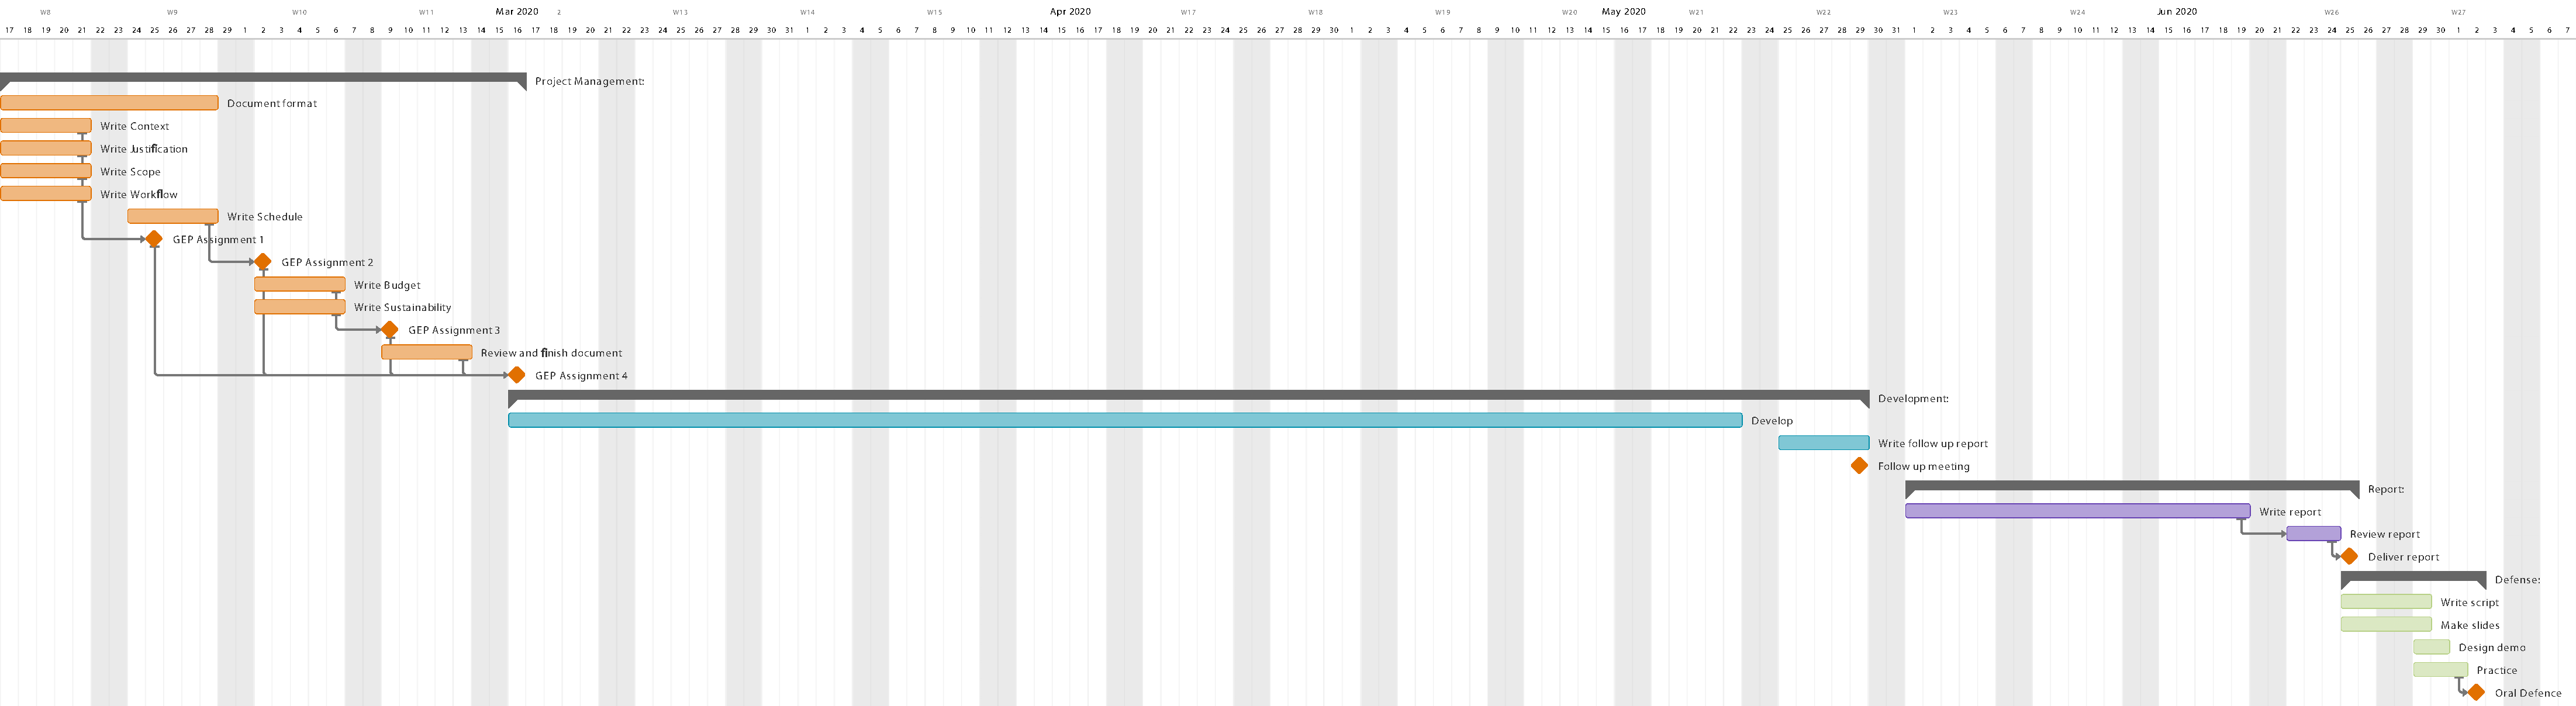
\includegraphics[width=\textheight-79pt,angle=90]{media/diagrams/gantt2.pdf}
    \caption{Updated Gantt diagram}
    \label{updated-gantt}
\end{figure}

\section{Budget}
\label{sec:budget}
% GradeCalc was born as a hobby project, therefore all the costs are minimized as much as possible.

\subsection{Human resources costs}
This is an open-source project driven by free contributions from the community. The project will start with only one contributor, me, but many people may get involved at some point. Because no one will get paid, the human resources costs will be \textbf{0€}. Nonetheless, I can estimate how much would this cost if people got hired to develop it, but I won't consider them in the total project sum.

\begin{table}[h!]
\centering
\begin{tabular}{lrrrr}
    \toprule
    \textbf{Rol} & \textbf{Weekly hours} & \textbf{Pay} & \textbf{Gross salary} & \textbf{Expense} \\
    \midrule
    Project Manager & 10h & 25€/h & 1000€/month & 1300€/month \\
    Front-end developer & 20h & 20€/h & 1300€/month & 2080€/month \\
    Full-stack developer & 20h & 20€/h & 1300€/month & 2080€/month \\
    \midrule
    \textbf{Total} & \textbf{50h} & & \textbf{4200€/month} & \textbf{5460€/month} \\
    \bottomrule
\end{tabular}
\caption{Ideal team}
\label{ideal-team}
\end{table}
I estimated that a 30\% of the gross salary is paid to Social Security.
\[Expense=GrossSalary\times1.3\]

According to the Gantt diagram \ref{gantt}, this team would be working for 6 sprints. This translates to 3 months, meaning that the total human resources costs would be 16380€. 

It's important to mention that they would do many more tasks than the ones I'll be able to do alone, so the planning would end up looking very different and the estimations I made inapplicable. Also, the Memory Writing, Report, and Defense blocks wouldn't make sense to have, so they would have even more sprints, increasing this cost.

\subsubsection{Salaries}

The total compensation per year of a \textbf{Project Manager} in Barcelona ranges between \textbf{22K€ and 58K€} \cite{project-manager-salary}. I chose 25€/h (\textbf{52K€}) because it's in that range.

The total compensation per year of a \textbf{Front End Developer} in Barcelona ranges between \textbf{19K€ and 40K€} \cite{front-end-salary}. I chose 20€/h (\textbf{41.6K€}) that is slightly above that range because the developer will also take extra responsibilities.

The total compensation per year of a \textbf{Full Stack Developer} in Barcelona ranges between \textbf{19K€ and 42K€} \cite{full-stack-salary}. I chose 20€/h (\textbf{41.6K€}) because it's in that range. I also thought that having similar salaries would be fairer for everyone on the team.

\subsubsection{Why that team?}

The Project Manager would be in charge of things like optimizing team performance, defining requirements, unblocking the others, having a larger picture of the project.

The Front-end developer would be an expert on the javascript framework chosen and answer questions that the other developer may need.

Because most of the work will be in the front-end and the back-end is very little, a full-stack would do the little back-end available first.

\newpage
\subsection{Hardware costs}
\label{sec:hardware}
Regarding hardware a similar thing happens, no specific hardware will be bought for this project and everything is going to be reused so hardware costs will be \textbf{0€} also. If the developers don't have it they just don't collaborate or someone else tests the app. The hardware I'm actually going to use is:
\begin{multicols}{2}
\begin{itemize}
    \item My laptop, a Surface Pro 2018
    \item My phone, a Google Pixel 2 XL.
    \item Sporadically, iPhones from friends.
    \item Sporadically, laptops from friends.
\end{itemize}
\end{multicols}
 But, again I can estimate the costs in case all the hardware had to be bought.

\begin{table}[h!]
\centering
\begin{tabular}{llrrrr}
    \toprule
    \textbf{Item} & \textbf{Model} & \textbf{Amount} & \textbf{Cost} & \textbf{Useful life} & \textbf{Expense} \\
    \midrule
    Laptop & Apple MacBook Pro 2019 & 3 & 4500€ & 5 years & 75€/month \\
    Mobile & Google Pixel 4 XL & 1 & 760€ & 3 years & 21.11€/month \\
    Mobile & Apple iPhone 11 & 1 & 630€ & 4 years & 13.13€/month \\
    \midrule
    \textbf{Total} & & & \textbf{3890€} & & \textbf{108.24€/month} \\
    \bottomrule
\end{tabular}
\caption{Ideal hardware}
\label{ideal-hardware}
\end{table}

The VAT of the hardware could be saved if they are bought by a company.
And if this is too much to pay, older or second-hand devices can be bought instead. Once the project finishes all hardware has to be sold to be afforded.

\subsubsection{Why those devices?}

To test the web app developers would need different operating systems and browsers. To test all browsers with a >2\% usage and 81\% global coverage, the web app needs to run in these browsers (Table \ref{browser-list-table}).

\begin{table}[h!]
\centering
\begin{tabular}{lrr}
    \toprule
    \textbf{BROWSER}& \textbf{USAGE} \\
    \midrule
    \textbf{Mobile Browsers} & \textbf{48.17\%} \\
    \midrule
    \hspace{3mm}Chrome for Android 78 & 34.26\% \\
    \hspace{3mm}UC Browser for Android 12.12 & 2.20\% \\
    \hspace{3mm}iOS Safari 13.3 & 9.29\% \\
    \hspace{3mm}Samsung Internet 10.1 & 2.42\% \\
    \midrule
    \textbf{Desktop Browsers} & \textbf{32.42\%} \\
    \midrule
    \hspace{3mm}Chrome 79 & 16.86\% \\
    \hspace{3mm}Chrome 80 & 10.66\% \\
    \hspace{3mm}Firefox 70 & 2.05\% \\
    \hspace{3mm}Safari 13 & 2.85\% \\
    \midrule
    \textbf{Total} & \textbf{80.79\%} \\
    \bottomrule
\end{tabular}
\caption{Browsers with more than >2\% usage \cite{browserl.ist}}
\label{browser-list-table}
\end{table}

All those browsers can be installed in macOS, iOS, and Android. So with a MacBook, an iPhone, and a Pixel, we can perform tests in all of them. Those devices are the newest ones when buying them, so they will last longer and get outdated latter.

Developers will use the same laptop to code the app. They could do this with any laptop. All tasks can be done with these devices.

\newpage
\subsection{Software costs}

This project free software as much as possible: Git, GitHub, Jira, Netlify, Firebase, Algolia, Travis CI, Figma, Google Analytics, VS Code, Overleaf, Linux...
The only unavoidable cost is the domain registration. GradeCalc uses a .app domain which costs \textbf{15€/year}, slightly more than a .com or .net domain. This is the only software expense by now, but if the app gets a lot of traffic it may get extra charges.

Most of the services that this project uses are free until a certain point. From that point the price increases drastically. The following software needs to be looked after to avoid unexpected charges:
\begin{itemize}
    \item \textbf{Firebase}: The free tear is enough, if the app doesn't waste reads/writes to firestore.  \url{https://firebase.google.com/pricing}
    \item \textbf{Algolia}: May not be enough. \url{https://www.algolia.com/pricing/}
    \item \textbf{Jira}: The free tear is enough. \url{https://www.atlassian.com/software/jira/pricing}
    \item \textbf{Netlify}: The free tear is enough. \url{https://www.netlify.com/pricing/}
\end{itemize}

\begin{table}[h!]
\centering
\begin{tabular}{llr}
    \toprule
    \textbf{Service} & \textbf{Plan} & \textbf{Cost} \\
    \midrule
    Domain & Domain Renewal & 15€/year \\
    Firebase & Spark Plan & Free \\
    Algolia & Community & Free \\
    Jira & Free & Free \\
    Netlify & Starter & Free \\
    \midrule
    \textbf{Total} & & \textbf{1.25€/month} \\
    \bottomrule
\end{tabular}
\caption{Software expenses}
\label{service-costs-table}
\end{table}

\newpage
\subsection{Other costs}

The project is going to be done with my current resources. But, again, simulating that a team would be hired, they would need a place to work. Barcelona offers coworking spaces for small companies or temporal projects, which fit perfectly this project. BarcelonaNavigator.com has an up-to-date list of recommended coworking spaces in Barcelona, from there I found SOWO that offers the Mini Flex rate \cite{coworking} that fits our needs:
\begin{multicols}{2}
\begin{itemize}
    \item \textbf{Flexible Desk}
    \item \textbf{1h Meeting rooms}
    \item \textbf{Access from 8:30-13:30h} \newline or from 14:00-19:00h
    \item Electricity and water included
    \item Internet connection
    \item Common areas access
    \item Coffee, water and snacks free
    \item 50 B/W prints
    \item Central location
\end{itemize}
\end{multicols}

\begin{table}[h!]
\centering
\begin{tabular}{lllr}
    \toprule
    \textbf{Service} & \textbf{Rate} & \textbf{Company} & \textbf{Cost} \\
    \midrule
    Co-working space & Mini Flex \cite{coworking} & SOWO & 140€/month + VAT \\
    \midrule
    \textbf{Total} & & & \textbf{140€/month + VAT} \\
    \bottomrule
\end{tabular}
\caption{Indirect expenses}
\label{other-costs-table}
\end{table}

\newpage
\subsection{Cost contingency}

10\% of the estimated costs would be saved to pay for unexpected expenses.

\begin{table}[h!]
\centering
\begin{tabular}{lrrr}
    \toprule
    \textbf{Category} & \textbf{Cost} & \textbf{Percentage} & \textbf{Contingency} \\
    \midrule
    Human resources & 5460.00€/month & 10\% & 546.00€/month \\
    Hardware & 58.24€/month & 10\% & 5.83€/month \\
    Software & 1.25€/month & 10\% & 0.13€/month \\
    Other & 140.00€/month & 10\% & 14.00€/month \\
    \midrule
    \textbf{Total} & & & \textbf{586€/month} \\
    \bottomrule
\end{tabular}
\caption{Contingencies expenses}
\label{contingency-costs-table}
\end{table}
\subsection{Unforeseen and extraordinary costs}

The main risk is spending too much time learning instead of coding, to mitigate that, the planning sets on each sprint a reasonable time to learn. But maybe it's not enough.

In terms of the project, if this happened the less important tasks would be skipped. This solution wouldn't add any extra cost at the expense of a less complete app.

If the project was developed by a team and they go too slow to finish, they would work for one extra month or add a new member.
\[MonthCost=HumanResources+Hardware+Software+Other+Contingencies\]
\begin{table}[h!]
\centering
\begin{tabular}{lrrr}
    \toprule
    \textbf{Event} & \textbf{Event cost} & \textbf{Odds} & \textbf{Cost} \\
    \midrule
    Extra month & 6295.49€ & 50\% & 3147.75€ \\
    \midrule
    \textbf{Total} & & & \textbf{3147.75€} \\
    \bottomrule
\end{tabular}
\caption{Unforeseen expenses}
\label{extra-costs-table}
\end{table}

\newpage
\subsection{Total costs}

\begin{table}[ht!]
\centering
\begin{tabular}{lrrr}
    \toprule
    \textbf{Category} & \textbf{Category cost} & \textbf{Amount} & \textbf{Total cost}\\
    \midrule
    Human resources & 5460€/month & 3months & 16380.00€ \\
    Hardware & 3890€ & 1 & 3890.00€ \\
    Software & 15€/year & 5year & 75.00€ \\
    Other & 140€/month & 3months & 420.00€ \\
    Contingencies & 586€/month & 3months & 1758.00€ \\
    Unforeseen & 3147.75€ & 1 & 3147.75€ \\
    \midrule
    \textbf{Total} & & & \textbf{25670.75€} \\
    \bottomrule
\end{tabular}
\caption{Total expenses}
\label{contingency-costs-table}
\end{table}

\newpage
\subsection{Management control}

To ensure the compliance of the initial budget, during the sprint review (\ref{sec:sprint-review}) at the end of each sprint I will calculate:
\begin{itemize}
    \item Human resources costs deviation.
    \item General costs deviation.
    \item Unforeseen costs deviation.
    \item Total costs until this point.
\end{itemize}

The deviations are going to be calculated with the following formulas:
\[Budget=HumanResources + Hardware + Software + Others + Contingencies + Unforessn\]
\[Estimated=Budget-Contingencies-Unforeseen\]
\[Deviation=Estimated-Real\]
\[UsedBudget=\frac{CurrentlySpent}{Estimated}\times100\%\]
The \textit{UsedBudget} should grow suddenly at the beginning, due to the hardware and software acquisition, and then grow linearly until 100\%. If we observe a different growing rate more money than estimated is being spent.

\subsection{Changes in the budget}

Although the planning changed a bit, the hours spent, the material used, and the services used are the same, so the costs don't vary.

\section{Sustainability}
\subsection{Self-assessment}
After answering the sustainability analysis survey, I've realized that in any project there is a sustainability component divided into three different dimensions: economic, environmental, and social. It has also made me think about the causes, consequences, and possible solutions about social, environmental, and economical problems that affect all kinds of IT projects.
I also contemplated the importance of suggesting ideas and applying solutions to this project to make it more sustainable.

Not only I chewed over the importance of sustainability in a project like this one, but also I realized the importance I was giving to this topic was not enough in my past projects, as result of a little knowledge about topics like the environmental costs that IT products have over their lifespan. I neither knew how to measure the environmental impact of Information and communications technology in the world. And I also didn't know the existence of sustainable technologies applicable to a software project.
I already knew the importance of introducing social justice, equity, diversity, and transparency in IT projects.

To conclude, this project has made me reflect on the
the importance of taking into account sustainability when developing a project from all perspectives; economically, environmentally, and socially.

\subsection{Economic Dimension}
\noindent \textbf{Regarding PPP: Reflection on the cost you have estimated for the completion of the project}

The estimated cost of the project only includes essential resources, in this case, 0. I'm going to reuse all the hardware I currently own and sporadically use my friends' devices to test the app.


\noindent \textbf{Regarding Useful Life: How are currently solved economic issues (costs...) related to the problem that you want to address (state of the art)?}

All current solutions have a similar architecture, all of them are websites or apps without a database or a really simple one.
So, their costs must be the domain registration and hosting.

\noindent \textbf{Regarding Useful Life: How will your solution improve economic issues (costs ...) with respect to other existing solutions?}

I'm going to use many free services at the beginning, and scale the project with also free or cheap services.

\subsection{Environmental Dimension}

\noindent \textbf{Regarding PPP: Have you estimated the environmental impact of the project?}

This project won't cause any environmental impact directly, it's an app to solve a quotidian problem more efficiently.
It may have an indirect impact due to the services it uses, none of them has a bad reputation on managing its resources.

\noindent \textbf{Regarding PPP: Did you plan to minimize its impact, for example, by reusing resources?}

Yes, as explained earlier in section \ref{sec:hardware}, all hardware is reused.

\noindent \textbf{Regarding Useful Life: How is currently solved the problem that you want to address (state of the art)? and how will your solution improve the environment with respect to other existing solutions?}

Any of these projects produce any waste, and my solution is no different.

\newpage
\subsection{Social Dimension}

\textbf{Regarding PPP: What do you think you will achieve -in terms of personal growth- from doing this project?}

I'll learn new technologies, tools, and techniques. Having real users using the app makes me set higher standards, giving me the motivation to do everything as good as possible.

\noindent \textbf{Regarding Useful Life: How is currently solved the problem that you want to address (state of the art)?, and how will your solution improve the quality of life (social dimension) with respect other existing solutions?}

This project is about making life easier for its users. The current solutions are very inconvenient and that's why this project was born. This topic is explained in-depth in section \ref{chap:intro}.

\noindent \textbf{Regarding Useful Life: Is there a real need for the project?}

Yes, there is. Although the problem that solves isn't critical.

\clearpage\newpage
\section{Laws and regulations}
\label{sec:laws}

% One particular detail that needs to be clarified about the project is the use of personal data.

The most important law that this project needs to follow is the GDPR\footnote{General Data Protection Regulation}\cite{gdpr}. It's the core of Europe's digital privacy legislation. 
Another similar regulation like the CCPA\footnote{California Consumer Privacy Act} can be considered, but the GradeCalc core users reside in Europe, where it doesn't apply.

To understand the GDPR it's really important to comprehend these two definitions\cite{gdpr-definitions}:
\begin{quote}
(1) ‘\textbf{personal data}’ means any information relating to an identified or identifiable natural person (‘data subject’); an identifiable natural person is one who can be identified, directly or indirectly, in particular by reference to an identifier such as a name, an identification number, location data, an online identifier or to one or more factors specific to the physical, physiological, genetic, mental, economic, cultural or social identity of that natural person;
\end{quote}

\begin{quote}
(2) ‘\textbf{processing}’ means any operation or set of operations which is performed on personal data or on sets of personal data, whether or not by automated means, such as collection, recording, organisation, structuring, storage, adaptation or alteration, retrieval, consultation, use, disclosure by transmission, dissemination or otherwise making available, alignment or combination, restriction, erasure or destruction;
\end{quote}

The only information stored in the database that could be considered as personal data by the GRPD\cite{gdpr} are the grades and the subject's creator id and name, explained in section \ref{sec:data-model}. Other information stored such as subject evaluation criteria and general information like name, color, and date is not personal, thus it's not regulated by this law.

In order to be GDPR compliant the app needs to have:
\begin{itemize}
    % \item An agreement checkbox (unchecked by default) that the user must check to register.
    \item A message above the login button that says something similar to "by clicking the Sign in button, I accept the terms and conditions".
    \item Have a page that explains how the personal data is processed (Privacy Policy).
    \item Have a page that explains how users can perform their rights, regarding GDPR, like erasure, portability, rectification, access, and restriction of the processing.
\end{itemize}

GradeCalc doesn't need a cookie banner because although using Google Analytics, the information that it collects is anatomized and basic.

If a user wants to perform any of the GDPR rights he/she just has to send an email to the provided address in the Privacy Policy page, and the administrator (in this case myself) will fulfill the request.

The third parties involved in this project are all GDPR compliant, so they can be used legally without any problem. Firebase is the most important external entity because it's the one processing the personal data, I had to verify that it is GDPR compliant\cite{firebase-gdpr} before using it.

\vspace*{\fill}
\begin{center}
    \includegraphics[height=8\fontcharht\font`\X]{media/gdpr.png}
\end{center}
\vspace*{\fill}
\chapter{REQUIREMENTS AND SPECIFICATION}
\label{chap:requirements}

% GradeCalc aims to be the first choice of students. To be in that precious spot, it will have to fit the student's needs perfectly. The following ones are the requirements I collected from asking colleagues and filtering brainstormed ideas.

This section defines and explains the requirements of the application. They are obtained by analyzing how students manage their grades and coming up with solutions that would help them be more productive. They are also obtained by directly asking what potential users would want in the app.

\section{Functional requirements}
\label{sec:user-stories}

This section presents the requirements of the app in the form of user stories (US).

% \begin{titlebox}{TODO}
%   Use some sort of table and for each requirement set: id, title, description, acceptation criteria
% \end{titlebox}

% \begin{titlebox}{TODO}
%   Add acceptation criteria
% \end{titlebox}

% Criteris d'acceptacio son molt importants, posar un google forms inventat

% no cal model de comportament

\nextUserStory{Calculate needed grade}\label{us:x}
\usStatement{user}{calculate needed grade to pass a course}{decide how much to study}

\nextUserStory{Calculate final grade}\label{us:x}
\usStatement{user}{calculate my final grade assuming a 0 in the remaining exams}{know if I already passed}

\nextUserStory{Current grades}\label{us:x}
\usStatement{user}{see my current grades}{view my performance}

\nextUserStory{Sign-up}\label{us:x}
\usStatement{user}{sign-up with an external authentication provider}{register faster and more conveniently.}

\nextUserStory{Log-in and Log-out}\label{us:x}
\usStatement{user}{log-in and Log-out}{decide when to use my account}

\nextUserStory{Save grades in my account}\label{us:x}
\usStatement{user}{save grades in my account}{share them between my desktop and mobile}

\nextUserStory{Save grades in the device}\label{us:x}
\usStatement{user}{save grades in the device}{use the app without an account or offline}

\nextUserStory{Create subject}\label{us:x}
\usStatement{user}{create subject}{use the app with any of my courses}

\nextUserStory{Edit subject}\label{us:x}
\usStatement{user}{edit subject}{correct mistakes or tweak values}

\nextUserStory{View subject}\label{us:x}
\usStatement{user}{view subject details}{see clearly all it's information}

\nextUserStory{Delete subject}\label{us:x}
\usStatement{user}{delete subject}{focus on other subjects}

\nextUserStory{Search subjects}\label{us:x}
\usStatement{user}{search subjects}{avoid creating them and save time}
% typos
% instant

\nextUserStory{Multiple evaluations}\label{us:x}
\usStatement{user}{be able to set have multiple evaluation formulas on subjects}{represent my subject's evaluation precisely}
% can share exams
% can have unique exams

% \nextUserStory{Subjects can have optional exams}\label{us:x}
% \usStatement{user}{subjects can have optional exams}{}

% \nextUserStory{Subjects' evaluations can share exams}\label{us:x}
% \usStatement{user}{subjects' evaluations can share exams}{}

\nextUserStory{Dashboard}\label{us:x}
\usStatement{user}{have a dashboard with my subjects}{handily input my grades}

% \nextUserStory{Quick view of my current grades (subject bar)}\label{us:x}
% \usStatement{user}{quick view of my current grades (subject bar)}{}

\nextUserStory{Auto-evaluate}\label{us:x}
\usStatement{user}{automatically reevaluate the calculations}{see the right values all the time}

\nextUserStory{Auto-save}\label{us:x}
\usStatement{user}{automatically save my changes}{save time saving and don't forget to save}

\nextUserStory{Auto-sync}\label{us:x}
\usStatement{user}{automatically syncs my changes with my account}{have a consistent state always}

\nextUserStory{Responsive UI}\label{us:x}
\usStatement{user}{have UI designed for mobile and desktop}{use the app in any screen size}

\nextUserStory{Use from browser}\label{us:x}
\usStatement{user}{use the app from the browser}{use it without downloading it}

\nextUserStory{Lunch icon}\label{us:x}
\usStatement{user}{have a lunch icon on the home screen}{quickly open the app}
% install from browser
% install from play store

% \nextUserStory{Install from browser}\label{us:x}
% \usStatement{user}{install the app from the browser}{quickly open the app}

% \nextUserStory{Download from Play Store}\label{us:x}
% \usStatement{user}{download the app from the Google Play Store}{download it like any other app}

\nextUserStory{Offline}\label{us:x}
\usStatement{user}{use the app offline}{use it without depending on my internet connection}

\nextUserStory{SEO}\label{us:x}
\usStatement{user}{find the app in Google}{open it without knowing the domain}

\nextUserStory{Tutorial}\label{us:x}
\usStatement{user}{have a tutorial}{learn to use the app the first time I visit it}

\nextUserStory{Undo}\label{us:x}
\usStatement{user}{be able to undo some actions}{fix mistakes}

\nextUserStory{Notifications}\label{us:x}
\usStatement{user}{be notified with tips and suggestions inside the app}{take advantage the app,  and use it correctly}

\nextUserStory{Accessible}\label{us:x}
\usStatement{user}{still be able to use the app if I have a disability}{use the app without complications}

\nextUserStory{Updates}\label{us:x}
\usStatement{user}{receive frequent updates}{enjoy the latest features}
% this sets CD

\nextUserStory{Analytics}\label{us:x}
\usStatement{user}{give data of my usage up (anonymized)}{improve the app}

% \nextUserStory{Implement Continuous Integration and Deployment}\label{us:x}
% \usStatement{user}{implement Continuous Integration and Deployment}{}

\nextUserStory{Open-source}\label{us:x}
\usStatement{user}{have the main code publicly available (open-source)}{validate that the app does what it states}

\nextUserStory{Background activity}\label{us:x}
\usStatement{user}{be aware of background activity}{better predict the behavior of the app}

\nextUserStory{In Spanish}\label{us:x}
\usStatement{user}{have the app entirely in Spanish}{understand it}

\nextUserStory{Legal page}\label{us:x}
\usStatement{user}{have a page with legal information}{solve any doubts}


% \nextUserStory{Create subject}\label{us:create-subject}
% \usStatement{user}{create a subject}{use it}
% US\ref{us:create-subject}



\clearpage\newpage
\section{Non-Functional requirements}
\label{sec:non-functional}

% \subsection{For the students}
% \begin{multicols}{3}
% \noindent
% Be \textbf{reliable}:
% \vspace{-5mm}
% \begin{itemize}[leftmargin=*]
%     \setlength\itemsep{-1em}
%     \item Don't lose data.
%     \item Don't miscalculate.
%     \item Keep grades private.
%     \item Work as expected.
%     \item Work on all devices.
%     \item Work offline.
% \end{itemize}
% \columnbreak
% \noindent
% Be \textbf{easy to learn} and use:
% \vspace{-5mm}
% \begin{itemize}[leftmargin=*]
%     \setlength\itemsep{-1em}
%     \item Simple and attractive UI.
%     \item Feel fast.
%     \item Place elements where expected.
%     \item Shows clearly where results come from.
% \end{itemize}
% \columnbreak
% \noindent
% Be \textbf{engaging}:
% \vspace{-5mm}
% \begin{itemize}[leftmargin=*]
%     \setlength\itemsep{-1em}
%     \item Get updates.
%     \item Have "cool" details.
%     \item Encourage to share the app.
%     \item Have an easy to remember name, logo, and domain.
% \end{itemize}

% \end{multicols}

% \subsection{For the developers}

% \begin{itemize}
%     \setlength\itemsep{-1em}
%     \item Have the minimum economic costs, zero if possible.
%     \item Use modern technologies.
%     \item Generate some economic income to pay for expenses.
%     \item Use open source technologies.
% \end{itemize}

This section highlights the 4 non-functional requirements (NFR) that the application must meet. These requirements shape the app so much that all features aim to satisfy them.

\subsection*{NFR 1 - Reliable}
\begin{itemize}
    \item \textbf{Description}: The functionalities have to work consistently and predictably, in other words, the app has to work as the user expects. For example, it doesn't lose data, it doesn't miscalculate, it works on all the user's devices, it works offline...
    \item \textbf{Justification}: The app has to work properly to be useful, otherwise there's no point in using it.
    \item \textbf{Acceptance criteria}: Ask a sample of users to evaluate, from 1 to 5, how much they agree to the following statements. A mean greater than 2.5 needs to be achieved.
    \begin{itemize}[noitemsep]
        \item The app works as I expect.
        \item The app does the calculations without mistakes.
        \item I can use the app from any of my devices.
        \item The app has never lost any of my data.
        \item I can use the app with the subjects I course.
    \end{itemize}
\end{itemize}

\subsection*{NFR 2 - Easy to use}
\begin{itemize}
    \item \textbf{Description}: The app has to be intuitive and accessible, in other words, easy to learn and easy to use.
    \item \textbf{Justification}: If the app is easy to use the users will save time and overall be more satisfied.
    \item \textbf{Acceptance criteria}: Ask a sample of users to evaluate, from 1 to 5, how much they agree to the following statements. A mean greater than 2.5 needs to be achieved.
    \begin{itemize}[noitemsep]
        \item The app is easy to learn
        \item The app is easy to use
        \item The app responds quickly to my actions.
        \item I know how to use the app in general.
        \item I know how to create a subject
        \item I understand all the information in the dashboard.
    \end{itemize}
\end{itemize}

\subsection*{NFR 3 - Engaging}
\begin{itemize}
    \item \textbf{Description}: The app must engage users and ensure that they are enjoying it and will recommend it.
    \item \textbf{Justification}: Happy users will attract new users helping the app grow. If the users are engaged, that means that the app is useful to them.
    \item \textbf{Acceptance criteria}: Ask a sample of users to evaluate, from 1 to 5, how much they agree to the following statements. A mean greater than 2.5 needs to be achieved.
    \begin{itemize}[noitemsep]
        \item I enjoy using the app.
        \item I would recommend the app.
        \item There's people using the app thanks to me.
        \item The app helps me to achieve my goals.
        \item The app helps me to pass the subjects.
        \item I open the app frequently.
        \item I open the app when I receive a new grade.
        \item GradeCalc's logo, name, and style are easy to remember.
        \item I like GradeCalc's logo, name, and style.
    \end{itemize}    
\end{itemize}

\subsection*{NFR 4 - Cheap to produce}
\begin{itemize}
    \item \textbf{Description}: The app has to be as cheap as possible to develop and maintain.
    \item \textbf{Justification}: This is a small hobby project developed by a student that is not willing to spend money on it unless it's imperceptible or would make a big difference.
    \item \textbf{Acceptance criteria}: the app must have a profit greater than -50€/year and cost less than 100€ to develop.
\end{itemize}


\section{Conceptual model}

The app has two main entities, subjects, and students, they are marked with thicker borders. 
\begin{itemize}
    \item Students are the users of the app and they can create and course subjects.
    \item Subjects are what students course that lead to an examination or qualification. A subject is taught in a faculty, and a faculty belongs to a university. Also, subjects are done in a course (usually a semester). 
    \item Faculty, university, and course are not relevant for the app's requirements, they are just related concepts, so in the database, they'll be just attributes of a subject, not standalone classes.
    \item A subject contains one or more evaluations and one or more exams. An evaluation contains exams with weights.
\end{itemize}

The main takeaway from the conceptual model (Fig. \ref{fig:conceptual-model}) is that students create and course subjects, and subjects have evaluations with exams and basic information to be searched like short name, full name, university or course. 

\vfill
\begin{figure}[ht!]
    \center
    \includegraphics[width=\linewidth]{media/diagrams/conceptual.pdf}
    \caption{Conceptual model's UML Diagram}
    \label{fig:conceptual-model}
\end{figure}
\vfill

\clearpage\newpage
\section{Tasks}

This section defines all the tasks to do in order to fulfill all the requirements that the application must meet. These tasks are very specific and can be directly placed into the Kanban board. They are organized by screens and components of the app. This section will help understand all the features implemented and it's level of detail.

% This section defines all the functional requirements that the application must meet.
% Overall, the app may look like it does a few things, but the ones it does are very polished. For example, the subject card alone has a tone of features, and looking at it in a glance seems that it must be trivial, but it has many small details that make the app truly productive and enjoyable. To come up with these requisites, there was an intense thought process to find the simplest way to present the features to the user.


\subsection*{Dashboard}
A user wants to see and interact with his subjects and grades.

\begin{itemize}[leftmargin=2cm]
    \item[\nextTask{}\label{req:x}] It is the homescreen of the app.
    \item[\nextTask{}\label{req:x}] It contains subject cards.
    \item[\nextTask{}\label{req:x}] When the app is opened, the subjects are retrieved from the device's local storage. And a non blocking spinner is shown while the subjects are being loaded.
    \item[\nextTask{}\label{req:x}]  When the app is opened and the user is logged-in, subjects are synced with his account. While this happens a non blocking spinner appears.
    \item[\nextTask{}\label{req:x}] The subject cards are sorted alphabetically by \textit{shortName}.
    \item[\nextTask{}\label{req:x}] When there are no subject cards, the add button starts a looping animation, similar to the rubberBand from the Animate.css\cite{animate-css} library, to draw attention.
    \item[\nextTask{}\label{req:x}] When there are no subject cards, the empty space is replaced with an explanatory text about the app. At the end of the text, there are instructions to add the first subject. This text serves two purposes, inform the user, and optimize the search engine indexing of the app.
    \item[\nextTask{}\label{req:x}] It has a header bar on top of the subject cards and in the top of the screen.
    \begin{itemize}[leftmargin=2cm]
        \item[\nextTask{}\label{req:x}] The header bar has, in the left, an icon that when clicked goes to the login screen.
        \item[\nextTask{}\label{req:x}] The header bar has, in the center, the app name.
        \item[\nextTask{}\label{req:x}] The header bar has, in the right, an icon that when clicked goes to the search subject screen.
    \end{itemize}
    \item[\nextTask{}\label{req:x}] It is responsive and the subjects are rearranged depending on the screen width.
    \item[\nextTask{}\label{req:x}] When all subject cards displayed are passed, a present appears at the bottom of the dashboard along with a congratulating text.
    \item[\nextTask{}\label{req:x}] When the gift is clicked a funny congratulating video appears at the bottom of the screen and plays automatically in a loop.
    \item[\nextTask{}\label{req:x}] If the app meets the PWA installation criteria\cite{pwa-install-criteria}, a notification shows up with the install action.
\end{itemize}

\subsection*{Subject card}
A user wants to work with a specific subject in the dashboard.

\begin{itemize}[leftmargin=2cm]
    \item[\nextTask{}\label{req:x}] It can be in collapsed or expanded state.
    \begin{itemize}[leftmargin=2cm]
        \item[\nextTask{}\label{req:x}] A subject card is collapsed by default.
        \item[\nextTask{}\label{req:x}] When a subject card is expanded it pushes the other ones instead of overlapping them.
        \item[\nextTask{}\label{req:x}] When a subject card is clicked where there's no intractable elements, it toggles its state from collapsed or expanded. The intractable elements are the subject bar, exam input, evaluation selector, edit icon and delete button.
        \item[\nextTask{}\label{req:x}] There's an animation for when a subject card is collapsed or expanded.
        \item[\nextTask{}\label{req:x}] A collapsed card doesn't show the exams' inputs nor the evaluation selector. And a expanded one does. 
    \end{itemize}
    \item[\nextTask{}\label{req:x}] It has a graphical representation of the selected evaluation, called \textit{subject bar}. The representation is a bar divided in sections where each section represents an exam and it's length is proportional to the exam weight.
    \begin{itemize}[leftmargin=2cm]
        \item[\nextTask{}\label{req:x}] In the subject bar, hovering a section shows a tooltip displaying the exam weight in percentage.
        \item[\nextTask{}\label{req:x}] In the subject bar, each section contains the exam name and the grade. If the exam is undone, it contains the necessary grade instead.
        \item[\nextTask{}\label{req:x}] In the subject bar, the done exams have the subject's color as background color.
        \item[\nextTask{}\label{req:x}] In the subject bar, the undone exams have a light background color.
        \item[\nextTask{}\label{req:x}] In the subject bar, the exams are sorted by same order that they are in the exam array of the evaluation. Not alphabetically nor per weight.
        \item[\nextTask{}\label{req:x}] In the subject bar, when a section is clicked it focuses the exam's input. If the card is collapsed it's also expanded.
        \item[\nextTask{}\label{req:x}] In the subject bar, when a section is to narrow to see the full grade or name, the first characters are visible. Instead of the characters in the middle. 
    \end{itemize}
    \item[\nextTask{}\label{req:x}] It has the final grade in big text.
    \begin{itemize}[leftmargin=2cm]
        \item[\nextTask{}\label{req:x}] The final grade is calculated by multiplying each exam grade by its weight and summing all the values. If an exam is undone a 0 is used in the calculation.
        \item[\nextTask{}\label{req:x}] The final grade is green if it's greater or equal than five and red otherwise.
        \item[\nextTask{}\label{req:x}] The final grade is rounded to two decimals.
        \item[\nextTask{}\label{req:x}] When the final grade passes from a number lower than five to one greater or equal to five a confetti animation is triggered. The animation shoots confetti over the subject card to congratulate the user. 
    \end{itemize}
    \item[\nextTask{}\label{req:x}] It has an evaluation selector if there are more than one.
    \begin{itemize}[leftmargin=2cm]
        \item[\nextTask{}\label{req:x}] When the evaluation is changed, the card updates instantly it's information (exam inputs, subject bar, final grade...).
        \item[\nextTask{}\label{req:x}] If an exam with the same name is in more than one evaluations, the grade is shared among them. It means that the same exam can be used in different evaluations.
        \item[\nextTask{}\label{req:x}] The application remembers what is the selected evaluation. If the user closes and opens the app again, the selected evaluation doesn't change.
    \end{itemize}
    \item[\nextTask{}\label{req:x}] It has the subject's \textit{shortName} in big text.
    \item[\nextTask{}\label{req:x}] It has an input field for each exam in the selected evaluation.
    \begin{itemize}[leftmargin=2cm]
        \item[\nextTask{}\label{req:x}] The inputs are grouped by their type attribute.
        \begin{itemize}[leftmargin=2cm]
            \item[\nextTask{}\label{req:x}] The type is styled like a subtitle.
            \item[\nextTask{}\label{req:x}] Next to the type, there's the sum of the weights of the exams with that type in percentage and rounded.
            \item[\nextTask{}\label{req:x}] The types are sorted by the same order that they are in the exam array of the evaluation. Not alphabetically nor per weight.
            \item[\nextTask{}\label{req:x}] The exam inputs inside the type are sorted by same order that they are in the exam array of the evaluation. Not alphabetically nor per weight.
        \end{itemize}
        \item[\nextTask{}\label{req:x}] The exam input has different styles depending on it's vaule.
        \begin{itemize}[leftmargin=2cm]
            \item[\nextTask{}\label{req:x}] When the exam input has a valid value, it's considered a \textit{done exam}. It has the subject's color as background.
            \item[\nextTask{}\label{req:x}] When the exam input has an empty value, it's considered an \textit{undone exam}. It has a gray background and it's placeholder is the necessary grade to pass.
            \item[\nextTask{}\label{req:x}] When the exam input is focused it has a black border.
            \item[\nextTask{}\label{req:x}] When the exam input's value isn't a number nor empty, it has a gray background with red borders. And it's considered an \textit{undone exam}.
            \item[\nextTask{}\label{req:x}] When the exam input's value is a number but lower than 0 or greater than 10, it has the subject's color as background with red borders. And it's considered a \textit{done exam}.
            \item[\nextTask{}\label{req:x}] If the exam has weight 0, it's hidden.
        \end{itemize}
        \item[\nextTask{}\label{req:x}] At the left of the input there's a label with it's name.
        \item[\nextTask{}\label{req:x}] The exam input only accepts numbers (digits, periods, commas, plus, minus and e for exponential). And in digital keyboards shows a numeric keyboard.
        \item[\nextTask{}\label{req:x}] The necessary grade is the necessary grade to receive in all the remaining undone exams to get a 5 in the final grade.
        \item[\nextTask{}\label{req:x}] Every time a grade is changed other information is updated instantly.
        \begin{itemize}[leftmargin=2cm]
            \item[\nextTask{}\label{req:x}] The necessary grade is updated.
            \item[\nextTask{}\label{req:x}] The final grade is updated.
            \item[\nextTask{}\label{req:x}] If the user is logged-in, the new grade is sent to his account.
        \end{itemize}
        \item[\nextTask{}\label{req:x}] The exam inputs take a reasonable space for their expected value length, usually less than 6 characters.
        % \item[\nextTask{}\label{req:x}] The exam inputs can have 10 characters at maximum.
    \end{itemize}
    \item[\nextTask{}\label{req:x}] It has a edit icon.
    \begin{itemize}[leftmargin=2cm]
        \item[\nextTask{}\label{req:x}] The edit icon has a hover animation.
        \item[\nextTask{}\label{req:x}] When clicked opens the edit subject screen of the current subject. With the title ``Edit subject'' and the action button ``Save''.
        \item[\nextTask{}\label{req:x}] If the user finally edits the subject, the subject card's information is updated instantly (name, color, exam inputs...).
        \item[\nextTask{}\label{req:x}] If the user finally edits the subject, and he's logged-in, the subject is also edited in his account.
    \end{itemize}
    \item[\nextTask{}\label{req:x}] It has a delete button.
    \begin{itemize}[leftmargin=2cm]
        \item[\nextTask{}\label{req:x}] Hovering the card displays the delete button.
        \item[\nextTask{}\label{req:x}] The delete button has tree animations. On show it fades in and scales up to normal. On hover it shakes. On click it scales down.
        \item[\nextTask{}\label{req:x}] When the delete button is clicked the card is deleted.
        \item[\nextTask{}\label{req:x}] When a card is deleted, the other cards move to their new locations and sizes in a smooth animation.
        \item[\nextTask{}\label{req:x}] When a card is deleted, a notification appears saying "You deleted \textit{subject's shortName}"\space and a action button says "undo". When the action is clicked the subject is restored, like nothing happened. If the user is logged-in, undoing the action re-adds the subject to his account.
        \item[\nextTask{}\label{req:x}] When a card is deleted, if the user is logged-in, the subject is also deleted from his account.
    \end{itemize}
\end{itemize}

\subsection*{Register, Log-in, and log-out}
A user wants to register, log-in, or log-out.

\begin{itemize}[leftmargin=2cm]
    \item[\nextTask{}\label{req:x}] When the user is logged-in, the user icon in the dashboard changes to his profile picture.
    \item[\nextTask{}\label{req:x}] When the user is logged-in, and a non blocking spinner is shown while the dashboard's subjects are being synced with the ones in the user's account.
    \item[\nextTask{}\label{req:x}] When the user is not logged-in, a notification shows up with the log-in action. Clicking the action does the same as clicking the log-in button in the log-in screen.
    \item[\nextTask{}\label{req:x}] The log-in screen is a popup in desktop and mobile.
    \begin{itemize}[leftmargin=2cm]
        \item[\nextTask{}\label{req:x}] It has the user's profile picture. If the user is not logged in, the picture is a default one. 
        \item[\nextTask{}\label{req:x}] It has the user's profile name. If the user is not logged in, the name is a default one (Anonymous). 
        \item[\nextTask{}\label{req:x}] It has a short text listing the benefits of logging-in.
        \item[\nextTask{}\label{req:x}] It has a log-in or log-out button, green and red respectively, depending on weather the user is logged in or not.
        \item[\nextTask{}\label{req:x}] The log-in button registers the user, without extra steps, if he is not registered yet.
    \end{itemize}
    \item[\nextTask{}\label{req:x}] The login system uses Google's log-in.
    \item[\nextTask{}\label{req:x}] When the app is opened, if the user was logged-in, he's logged-in automatically.
\end{itemize}

\subsection*{Edit subject}
A user wants to edit a subject

\begin{itemize}[leftmargin=2cm]
    \item[\nextTask{}\label{req:x}] The screen title can be changed.
    \item[\nextTask{}\label{req:x}] The action button label can be changed.
    \item[\nextTask{}\label{req:x}] When the action button is clicked the all inputs are read and a new subject object is crated. This object is returned to the previous screen, delegating the responsibility.
    \item[\nextTask{}\label{req:x}] It has a grid to edit the evaluation.
    \begin{itemize}[leftmargin=2cm]
        \item[\nextTask{}\label{req:x}] In the grid, each row represents an exam, and each extra column an evaluation.
        \item[\nextTask{}\label{req:x}] The fixed columns are the following: exam name, exam category and exam grade.
        \item[\nextTask{}\label{req:x}] There are extra columns, one per each evaluation. The first row of the column is the evaluation name, and each row the weight of the corresponding exam.
        \item[\nextTask{}\label{req:x}] The weight are in percentage without the \% symbol.
        \item[\nextTask{}\label{req:x}] If a weight is empty, it's considered 0.
        \item[\nextTask{}\label{req:x}] Below each evaluation column there's a label indicating the sum of all the weights of the evaluation. This way the users can check quickly that it adds to 100\%.
        \item[\nextTask{}\label{req:x}] In the grid, rows and columns can be added and removed.
        \begin{itemize}[leftmargin=2cm]
            \item[\nextTask{}\label{req:x}] There's a faded extra row at the bottom, and a faded extra column at the left. If the user types something in there, it becomes clear and part of the grid. A new faded row or column is added to let the user repeat the process.
            \item[\nextTask{}\label{req:x}] If the user deletes all the values of a row or column, it disappears.
        \end{itemize}
        \item[\nextTask{}\label{req:x}] The grid can be easily navigable with the keyboard.
        \item[\nextTask{}\label{req:x}] If the grid is to big to fit the screen, it can be scrolled.
        \item[\nextTask{}\label{req:x}] If the user clicks the action button and there isn't at least 1 exam a notification appears and the action is ignored.
        \item[\nextTask{}\label{req:x}] If the user clicks the action button and there isn't at least 1 evaluation a notification appears and the action is ignored.
    \end{itemize}
    \item[\nextTask{}\label{req:x}] It has a section with the subject information fields.
    \begin{itemize}[leftmargin=2cm]
        \item[\nextTask{}\label{req:x}] It has a field for: \textit{shortName}, \textit{longName}, \textit{course}, \textit{faculty} and \textit{university}.
        \item[\nextTask{}\label{req:x}] It has a field \textit{color} where the allowed colors are displayed and the user checks the one he wants. By default a random one is selected.
        \item[\nextTask{}\label{req:x}] Each field has it's label always visible.
        \item[\nextTask{}\label{req:x}] When the label is clicked the input is focused.
        \item[\nextTask{}\label{req:x}] The inputs have their sizes proportionate to the expected content length.
        \item[\nextTask{}\label{req:x}] The fields \textit{shortName}, \textit{longName}, \textit{course}, \textit{faculty} and \textit{university} can't be empty.
        \item[\nextTask{}\label{req:x}] The fields have the same style as the exam inputs.
        \item[\nextTask{}\label{req:x}] The field \textit{color} must have always be chosen.
        \item[\nextTask{}\label{req:x}] It has the \textit{creationDate} and \textit{creatorName} but they are not editable. They look like a text instead of a disabled input. The \textit{creationDate} is in format \texttt{d/m/yyyy}.
        \item[\nextTask{}\label{req:x}] When a field is invalid it has a red border.
        \item[\nextTask{}\label{req:x}] If the user clicks the action button and there are invalid fields a notification with appears with the name of the invalid field in the message and the action is ignored.
    \end{itemize}
    \item[\nextTask{}\label{req:x}] It looks like a popup in desktop and like a full page in mobile. It can be scrolled in both styles.
    \item[\nextTask{}\label{req:x}] If the user clicks the back button of the browser, the popup blurred background or the back arrow in the header bar, the changes are discarded and the app navigates to the last screen.
\end{itemize}

\subsection*{Search subject}
\begin{itemize}[leftmargin=2cm]
    \item[\nextTask{}\label{req:x}] It has a big search input.
    \begin{itemize}[leftmargin=2cm]
        \item[\nextTask{}\label{req:x}] The search input has an example as placeholder.
        \item[\nextTask{}\label{req:x}] Below the the search input there's a short text explaining what field are searchable.
        \item[\nextTask{}\label{req:x}] The search input is focused automatically when this screen is opened.
        \item[\nextTask{}\label{req:x}] When the search input has text, a cross icon appears at the right and when it's clicked it removes the input's content.
    \end{itemize}
    \item[\nextTask{}\label{req:x}] When the user types in the search input, the results appear in the screen.
    \begin{itemize}[leftmargin=2cm]
        \item[\nextTask{}\label{req:x}] When the user types a character, a search is performed automatically and the results displayed and updated instantly as the user writes.
        \item[\nextTask{}\label{req:x}] If there are no results, a text appears saying that there are no results.
        \item[\nextTask{}\label{req:x}] When there are results, the create button disappears.
        \item[\nextTask{}\label{req:x}] The search engine accepts typos.
        \item[\nextTask{}\label{req:x}] The results are sorted by relevance.
    \end{itemize}
    \item[\nextTask{}\label{req:x}] If there are results they are displayed in a list.
    \begin{itemize}[leftmargin=2cm]
        \item[\nextTask{}\label{req:x}] It contains a checkbox
        \begin{itemize}[leftmargin=2cm]
            \item[\nextTask{}\label{req:x}] The checkboxes are disabled by default.
            \item[\nextTask{}\label{req:x}] When the subject of the result is already added to the dashboard, the checkbox is checked but disabled.
            \item[\nextTask{}\label{req:x}] Clicking the checkbox checks or unchecks it with an animation.
            \item[\nextTask{}\label{req:x}] When the search query changes, the checked subjects stay checked although they are not visible. If they appear in another query they'll still be checked.
        \end{itemize}
        \item[\nextTask{}\label{req:x}] It contains the \textit{shortName}, \textit{longName}, \textit{course}, \textit{faculty} and \textit{university} attributes as text.
        \item[\nextTask{}\label{req:x}] The matching characters from the query are highlighted.
        \item[\nextTask{}\label{req:x}] It contains a edit icon that when clicked opens the edit subject screen of the current subject. With the title ``Edit and add subject'' and the action button ``Add'' that adds the subject directly with the changes. When clicked also checks the result checkbox.
    \end{itemize}
    \item[\nextTask{}\label{req:x}] When the action button is clicked the checked subjects are added to the dashboard.
    \item[\nextTask{}\label{req:x}] If the user is logged-in, when the action button is clicked the checked subjects are also added to the user's account.
    \item[\nextTask{}\label{req:x}] When the action button is clicked, while the subjects are being added, a non blocking spinner informs that the subjects are being added in the background.
    \item[\nextTask{}\label{req:x}] It has a create button.
    \begin{itemize}[leftmargin=2cm]
        \item[\nextTask{}\label{req:x}] There's a short explanatory text of what creating a new subject means.
        \item[\nextTask{}\label{req:x}] When the create button is clicked it opens the edit subject screen of an empty subject. 
        \begin{itemize}[leftmargin=2cm]
            \item[\nextTask{}\label{req:x}] The edit screen has as title ``New subject'' and as action button ``Create'' that creates and adds the subject to the dashboard.
            \item[\nextTask{}\label{req:x}] If the user is logged-in, the subject is also created in the database. 
            \item[\nextTask{}\label{req:x}] While the subjects are being added, a blocking spinner informs that the subjects are being created.
        \end{itemize}
        \item[\nextTask{}\label{req:x}] The create button doesn't draw a lot of attention. To prevent unnecessary clicks.
    \end{itemize}
    \item[\nextTask{}\label{req:x}] It looks like a popup in desktop and like a full page in mobile. It can be scrolled in both styles.
    \item[\nextTask{}\label{req:x}] If the user clicks the back button of the browser, the popup blurred background or the back arrow in the header bar, the changes are discarded and the app navigates to the last screen.
\end{itemize}

\subsection*{Notifications}
A user wants to be notified of certain things and be able to respond with an action.

\begin{itemize}[leftmargin=2cm]
    \item[\nextTask{}\label{req:x}] It has a message that can be changed.
    \item[\nextTask{}\label{req:x}] It has an action name and callback function that can be changed.
    \item[\nextTask{}\label{req:x}] It appear for 8 seconds by default and can be changed.
    \item[\nextTask{}\label{req:x}] It has a slide up animation when appears.
    \item[\nextTask{}\label{req:x}] It has a slow fade out animation to inform the user how much time is remaining until it disappears, instead of disappearing instantly.
    \item[\nextTask{}\label{req:x}] If it has a action, after disappearing it can still be clicked for 0.5 seconds, although it's not visible. It's a grace second, in case the user clicked it too late.
    \item[\nextTask{}\label{req:x}] It's placed on top of everything at the bottom center of the screen.
\end{itemize}

\subsection*{Spinners}
A user wants to be notified of background processes.

\begin{itemize}[leftmargin=2cm]
    \item[\nextTask{}\label{req:x}] The non blocking spinners appear at the bottom of the dashboard.
    \begin{itemize}[leftmargin=2cm]
        \item[\nextTask{}\label{req:x}] They are discrete
        \item[\nextTask{}\label{req:x}] They have a message.
    \end{itemize}
    \item[\nextTask{}\label{req:x}] The blocking spinners, are placed on top of everything (in the z dimension).
    \begin{itemize}[leftmargin=2cm]
        \item[\nextTask{}\label{req:x}] They have a message.
        \item[\nextTask{}\label{req:x}] They have a long and entertaining animation. To make the waiting more pleasant.
        \item[\nextTask{}\label{req:x}] If they take more than the expected time, a message shows up telling that something went wrong.
    \end{itemize}
\end{itemize}

\subsection*{General}
\begin{itemize}[leftmargin=2cm]
    \item[\nextTask{}\label{req:x}] The app's UI is entirely in Spanish.
    \item[\nextTask{}\label{req:x}] The app is a Progressive Web App (PWA).
    \item[\nextTask{}\label{req:x}] The app is published in a domain.
    \item[\nextTask{}\label{req:x}] The app is published in the Google Play Store.
    \item[\nextTask{}\label{req:x}] The app can work offline (exept logging-in, and searching subjects).
    \item[\nextTask{}\label{req:x}] The subjects are stored in the device's local storage and if logged-in in his account.
    \item[\nextTask{}\label{req:x}] The app is the first google result when searching "GradeCalc" and "Grade Calc".
    \item[\nextTask{}\label{req:x}] The main source code is open-source.
    \item[\nextTask{}\label{req:x}] The user account information can only be accessed by the own user.
    \item[\nextTask{}\label{req:x}] The subject's in the database can't be edited or deleted by users, but they can create new subjects.
    \item[\nextTask{}\label{req:x}] The decimal separator is always displayed with a period. When the user types a number can use indistinctly a period or a comma.
    \item[\nextTask{}\label{req:x}] The site uses Google Analytics.
    \item[\nextTask{}\label{req:x}] The app's deployment is automated.
    \item[\nextTask{}\label{req:x}] The app's testing is automated.
    \item[\nextTask{}\label{req:x}] The app has icons for most of the platforms (favicon, android, iOS...).
    \item[\nextTask{}\label{req:x}] The app has a privacy and policy page.
\end{itemize}

% \subsection*{Old}
% \begin{itemize}[leftmargin=2cm]
%     \item[\nextTask{}\label{req:x}] Calculate needed grade to pass a course.
%     \item[\nextTask{}\label{req:x}] User can set custom needed grade, instead of just a 5.
%     \item[\nextTask{}\label{req:x}] Calculate final grade.
%     \item[\nextTask{}\label{req:x}] Sign-up with email, Google, GitHub, and Facebook.
%     \item[\nextTask{}\label{req:x}] Delete account.
%     \item[\nextTask{}\label{req:x}] Log-in and Log-out.
%     \item[\nextTask{}\label{req:x}] Save grades in an account (cloud) to share them between desktop and mobile.
%     \item[\nextTask{}\label{req:x}] Courses: Search, Create, View, Edit and Delete.
%     \item[\nextTask{}\label{req:x}] Courses can have a custom grade to pass.
%     \item[\nextTask{}\label{req:x}] Dashboard with course cards where users input their grades.
%     \item[\nextTask{}\label{req:x}] Achieve finished courses instead of deleting them.
%     \item[\nextTask{}\label{req:x}] Auto-evaluate calculations on change.
%     \item[\nextTask{}\label{req:x}] Auto-save changes.
%     \item[\nextTask{}\label{req:x}] UI designed for mobile and desktop.
%     \item[\nextTask{}\label{req:x}] Save grades in the device to use the app offline.
%     \item[\nextTask{}\label{req:x}] Have a lunch icon on the home screen.
%     \item[\nextTask{}\label{req:x}] Basic features work offline.
%     \item[\nextTask{}\label{req:x}] It is a Progressive Web App (PWA).
%     \item[\nextTask{}\label{req:x}] Create special evaluation formulas.
%     \item[\nextTask{}\label{req:x}] Courses can have multiple evaluation formulas.
%     \item[\nextTask{}\label{req:x}] Courses can have optional exams.
%     \item[\nextTask{}\label{req:x}] Be the first search result in search engines, especially Google.
%     \item[\nextTask{}\label{req:x}] Guided tour to learn to use the app the first time visiting it.
%     \item[\nextTask{}\label{req:x}] Support some none 1-10 grading systems like A-F, 1-5 and percentages.
%     \item[\nextTask{}\label{req:x}]  Multi-language (Spanish, English, and Catalan).
%     \item[\nextTask{}\label{req:x}] Share button.
%     \item[\nextTask{}\label{req:x}] Publish in Google Play Store.
%     \item[\nextTask{}\label{req:x}] Some actions can be undone.
%     \item[\nextTask{}\label{req:x}] UI banner that notifies important messages.
%     \item[\nextTask{}\label{req:x}] The app is accessible.
%     \item[\nextTask{}\label{req:x}] Set-up domain and deployment.
%     \item[\nextTask{}\label{req:x}] Collect metrics to improve the app.
%     \item[\nextTask{}\label{req:x}] Implement Continuous Integration and Deployment.
%     \item[\nextTask{}\label{req:x}] Be open source and accept contributions.
% \end{itemize}


\chapter{SOFTWARE DESIGN}
\label{chap:design}

\section{Software architecture}

This section explains the application's internal structure. 

\subsection{Logical architecture}

The application's architecture is multilayered, it uses the widespread three-tier architecture. This is a clear explanation of the three-tier architecture:

\begin{quote}
    Three-tier architecture is a client-server software architecture pattern in which the user interface (presentation), functional process logic ("business rules"), computer data storage, and data access are developed and maintained as independent modules, most often on separate platforms. \cite{multitier}
\end{quote}

In the case of this project, the presentation layer is the most important one with the majority of the code. The app focuses a lot on productivity, so most of the GradeCalc's features are on its interface. The domain layer has the app's logic, and the data layer is composed of the database structure and thanks to Firebase it doesn't have any code.

% \vfill
% \begin{figure}[H]
%     \center
%     
\includegraphics[width=0.25\columnwidth]{media/layers.pdf}
%     \caption{Three tier layers.}
% \end{figure}
% \vfill

\clearpage\newpage
\subsubsection{Design patterns}
\label{sec:patterns}

Design patterns are typical solutions to common problems in software design. Each pattern is like a blueprint that you can customize to solve a particular design problem in your code.\cite{refactoring-guru}

In this section, I'm going to explain and justify the design patterns that the software of this project uses. Identifying the design patterns leads to better code because they are proved to work. Coding a custom solution certain cases may be forgotten thous introducing bugs is more frequent.

\subsubsection*{Singleton}

Singleton is a creational design pattern that lets you ensure that a class has only one instance, while providing a global access point to this instance.\cite{refactoring-guru-singleton}

This pattern is used in the database connection object as recommended by the Cloud Firestore documentation\cite{firestore-doc-init}. The code doesn't enforce the use of a singleton, but the constructor is only called once. This approach is considered a better practice because singletons inherently cause code to be tightly coupled. This makes faking them out under test rather difficult in many cases. But not enforcing the "singletoness" of the class mitigates its issues.

\subsubsection*{Proxy}

Proxy is a structural design pattern that lets you provide a substitute or placeholder for another object. A proxy controls access to the original object, allowing you to perform something either before or after the request gets through to the original object.\cite{refactoring-guru-proxy}

This pattern is used to interact with the database. There's a class that provides methods for uploading data. This is good for testing because the class can be mocked to not use the real database connections when testing certain code.

\subsubsection*{Null object}

Null object is a behavioral design pattern that avoids null references by providing a default object.

This pattern is used in the login system, when the user is not logged in, the user information object contains a default name and picture. This name and picture are displayed in the user popup.

\subsubsection*{Servant}

Servant or Utility class is a structural design pattern that defines a class with common functionality for a group of classes. The helper classes generally have no objects hence they have all static methods that act upon different kinds of class objects.

This pattern is used specially for mathematical functions like: \mintinline{js}{random(min, max)} or \mintinline{js}{round(number, decimalPlaces)}; and other kind of generic tasks like: \mintinline{js}{getRandomID()} or \mintinline{js}{isEmpty(object)}.

\subsubsection*{Adapter}

Adapter is a structural design pattern that allows objects with incompatible interfaces to collaborate.\cite{refactoring-guru-adapter}

This pattern is seamlessly used when displaying information from JSON format into HTML format because the browser can only display HTML. For example, it is used when the user searches for a subject the response obtained is a JSON object that is transformed into HTML to be displayed.



% \begin{titlebox}{TODO}
%   (3 capes, dibuix, explcacio i els patrons) three-tier architecture
% \end{titlebox}




% -----------------------------------------------------------------------------------
% -----------------------------------------------------------------------------------
% -----------------------------------------------------------------------------------
% -----------------------------------------------------------------------------------
\newpage
\subsection{Physical architecture}

% \begin{titlebox}{TODO}
%   Fill content (les 3 capes estan al frontend, i el firebase esta separat, tb netlify) (explicar com es conecta)
% \end{titlebox}

The physical architecture is heavily influenced by the choice of using Firebase. Doug Stevenson explains how firebase shapes your app's architecture very well in his Medium article "What is Firebase? The complete story, abridged."\cite{firebase-article}, this is an extract of his article:

\begin{quote}
    \onehalfspacing
    Firebase is a toolset to “build, improve, and grow your app”, and the tools it gives you cover a large portion of the services that developers would normally have to build themselves, but don’t really want to build, because they’d rather be focusing on the app experience itself. This includes things like analytics, authentication, databases, configuration, file storage, push messaging, and the list goes on. The services are hosted in the cloud, and scale with little to no effort on the part of the developer.
\end{quote}
\begin{quote}
    \onehalfspacing
    This is different than traditional app development, which typically involves writing both frontend and backend software. The frontend code just invokes API endpoints exposed by the backend, and the backend code actually does the work. However, with Firebase products, the traditional backend is bypassed, putting the work into the client.
\end{quote}

\vfill
\begin{figure}[H]
    \center
    \includegraphics[width=0.95\columnwidth]{media/diagrams/firebase-diagram.png}
    \caption{Traditional vs Firebase architecture. \cite{firebase-article}}
    \label{fig:firebase-diagram}
\end{figure}
\vfill



\clearpage\newpage\noindent
The Firebase suite offers many individual products (Fig. \ref{fig:firebase-products}). The ones that this project uses are authentication and database.

\begin{figure}[H]
    \center
    \includegraphics[width=0.95\columnwidth]{media/firebase-products-cropped.png}
    \caption{Firebase products. \cite{firebase-article}}
    \label{fig:firebase-products}
\end{figure}

% GradeCalc uses Google Firebase as the back-end, from all the features it offers, GradeCalc uses authentication and database. GradeCalc also uses Algolia, a third-party service, to perform searches. There's a cron job\footnote{A cron job is a scheduled task that runs periodically.} in Heroku that runs every day to update the searchable information in Algolia. Notice that using Firebase and Algolia allows to not have any code in the back-end, so practically speaking GradeCalc has no back-end code.

\noindent
The 3 application layers are in the front-end. There we use Gulp to generate the needed and optimized static HTML, CSS, and JS files. These optimized files are hosted in Netlify.

\vfill
\begin{figure}[H]
    \center
    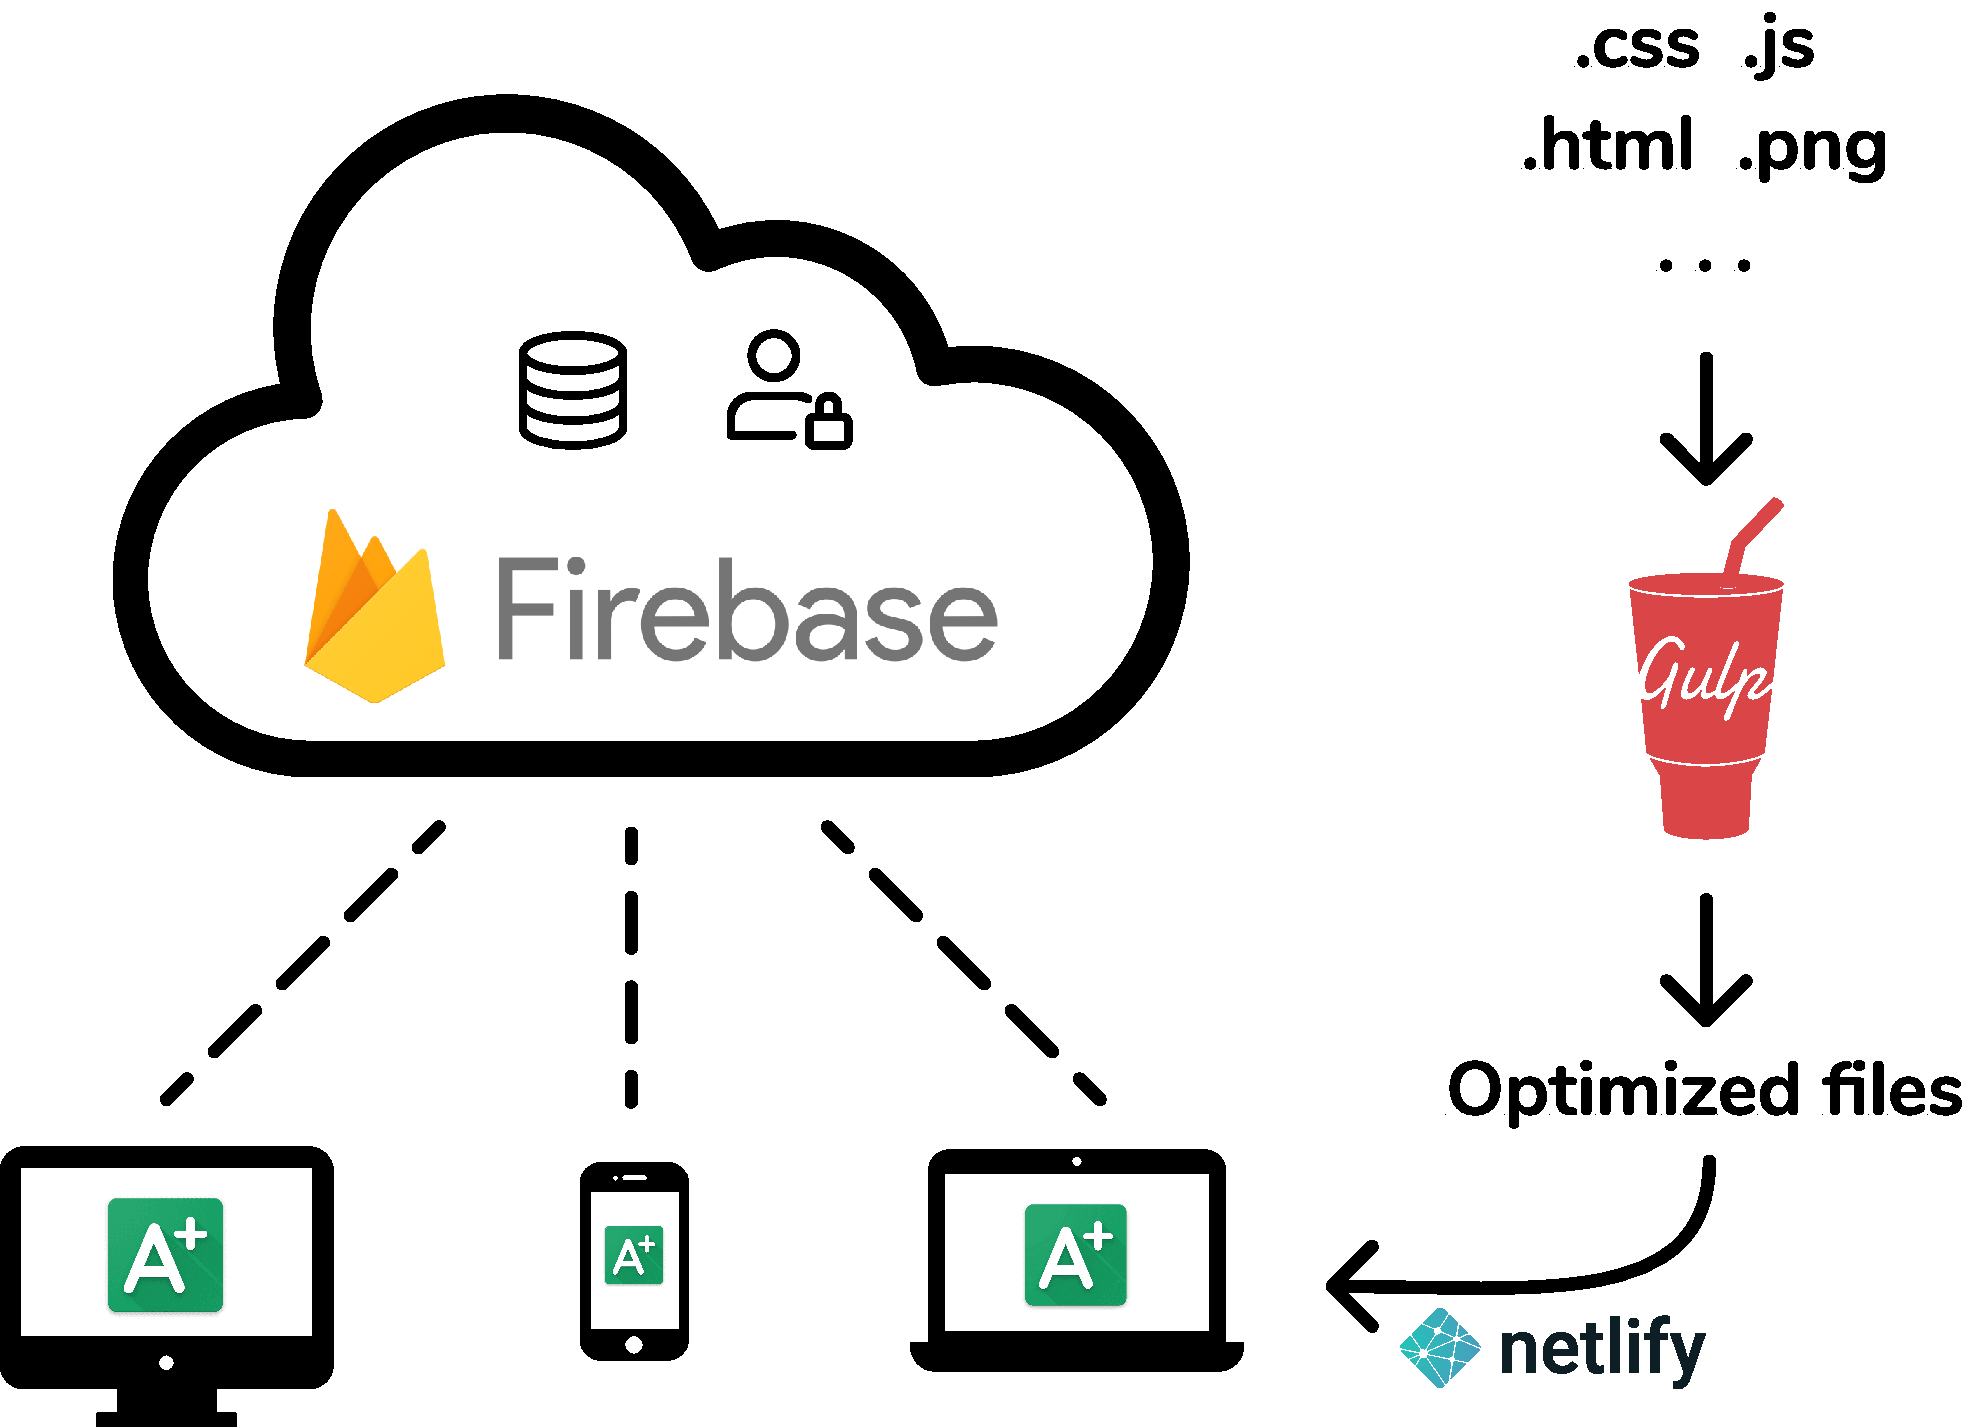
\includegraphics[width=0.85\columnwidth]{media/diagrams/architecture.pdf}
    \caption{GradeCalc architecture}
    \label{fig:architecture_diagram}
\end{figure}
\vfill





% \vfill
% \begin{figure}[H]
%     \center
%     \includegraphics[width=0.5\columnwidth]{media/diagrams/MVC-Process.pdf}
%     \caption{The model, view, and controller pattern relative to the user.\cite{mvc-diagram}}
%     \label{fig:mcv-diagram}
% \end{figure}
% \vfill





\clearpage\newpage\noindent
GradeCalc is a Progressive Web App (PWA) instead of a native app. This is how Mozilla Web Docs defines PWAs \cite{pwa-mozilla}:

PWAs are web apps developed using a number of specific technologies and standard patterns to allow them to take advantage of both web and native app features. There are some key principles a web app should try to observe to be identified as a PWA. It should be:

\begin{itemize}[noitemsep]
    \item \textbf{Discoverable}, so the contents can be found through search engines.
    \item \textbf{Installable}, so it can be available on the device's home screen or app launcher.
    \item \textbf{Linkable}, so you can share it by simply sending a URL.
    \item \textbf{Network independent}, so it works offline or with a poor network connection.
    \item \textbf{Progressive}, so it's still usable on a basic level on older browsers, but fully-functional on the latest ones.
    \item \textbf{Re-engageable}, so it's able to send notifications whenever there's new content available.
    \item \textbf{Responsive}, so it's usable on any device with a screen and a browser—mobile phones, tablets, laptops, TVs, refrigerators, etc.
    \item \textbf{Safe}, so the connections between the user, the app, and your server are secured against any third parties trying to get access to sensitive data.
\end{itemize}

\noindent
Offering these features and making use of all the advantages offered by web applications can create a compelling, highly flexible offering for your users and customers.

% \subsubsection*{What is a Single-page application?}
% A single-page application (SPA) is a web application or website that interacts with the web browser by dynamically rewriting the current web page with new data from the webserver, instead of the default method of the browser loading entire new pages. The goal is faster transitions that make the website feel more like a native app.

% In a SPA, all necessary HTML, JavaScript, and CSS code is either retrieved by the browser with a single page load, or the appropriate resources are dynamically loaded and added to the page as necessary, usually in response to user actions. The page does not reload at any point in the process, nor does it transfer control to another page, although the location hash or the HTML5 History API can be used to provide the perception and navigability of separate logical pages in the application. \cite{spa}

% \subsubsection*{What is a Progressive web app?}
% Progressive Web Apps are web applications that have been designed so they are capable, reliable, and installable. These three pillars transform them into an experience that feels like a native application. \cite{pwa-pillars}
% Where:
% \begin{itemize}[noitemsep]
%     \item \textbf{Capable} means that the PWA feels as powerful/capable as a native app.
%     \item \textbf{Reliable} means that the PWA feels fast and dependable regardless of the network.
%     \item \textbf{Installable} means that the PWA runs in a standalone window instead of a browser tab
% \end{itemize}

% \subsubsection*{Why PWA instead of a native app?}

GradeCalc is PWA mainly \textbf{because it saves up a lot of development time} at the expense of some, really specific, capabilities. A PWA can run in any of the most popular operating systems (Android, iOS, Windows, macOS, and Linux), contrary to a native app that only runs in its respective OS. So, the same code will work everywhere.

% None of the app requirements (\ref{chap:requirements}) are exclusive to native apps, and some are easily achieved with a PWA.

% The main downside is that iOS users won't fully enjoy the web app\cite{pwa-ios} because Safari iOS doesn't implement some of the APIs that PWAs use, like Push Notifications. As Chris Love explains \cite{pwa-ios}:
% \begin{displayquote}
% Sure there are limitations to for Progressive Web Apps on iOS, but they are not deal breakers. Many of the most requested features have at least some form of fallback solution. It may not provide a comparable user experience the native web platform API or service offers.
% \end{displayquote}



\clearpage\newpage
\section{Presentation layer's design}
This section explains the user interface and user experience design of the app.

\subsection{User Interface}
\label{sec:ui}

In this subsection, we'll go through the screens of the application showcasing what features do they implement and explaining how they work. All the screenshots are of the real application developed and working in production. 

\subsubsection{Dashboard and welcome}

The dashboard is the main screen of the app and also the entry point. Every time a user opens the app it goes to this screen.

On the top of the screen there's the header bar with three elements: the \inlineicon{icon-user.pdf} button that goes to the login screen (Fig. \ref{fig:login}), the app name in the middle, and the \inlineicon{icon-plus.pdf} button that goes to the search subject screen (Fig. \ref{fig:search-empty}).

The \inlineicon{icon-user.pdf} button turns into the user's profile picture if he's logged in.

On the main part of the screen, there are all the subjects that the student is coursing in the form of cards (Fig. \ref{fig:card}). By default all the cards are collapsed, like the \textit{XC} and \textit{IDI} ones in the example (Fig. \ref{fig:card}). The subject cards are explained in depth in section \ref{sec:subject-card}.

\clearpage\newpage
\noindent
In general, this is how to interpret what's going on in Figure \ref{fig:dashboard}:

The student is in the 4th semester of Computer Engineering in FIB UPC and he has most of the grades. 

In subject \textit{AC} he has done all the exams but he doesn't have the \textit{Laboratorio} grades yet, although he can be confident that he will pass because he needs just a 0.25 to pass. 

The same cannot be said for \textit{EEE}, he needs a 4.63 in the two last exams. He has the cursor on the \textit{PEC1} exam and he's typing and erasing numbers to see how the necessary grade changes, he skipped a few classes and he wants to know what grade he would need in the \textit{PEC2} exam if he gets a 3 or 4 in \textit{PEC1}, to see if it's viable.

By looking at the next card, \textit{IES}, we can see that he already passed, with at least a 6.9, regardless of the grade he gets in \textit{P}.

Finally, in \textit{IDI} he has good grades but the exam \textit{T2} weights so much that he still hasn't passed. \textit{T2} takes half of the space in the bar, meaning that his weight is also half of the total, that is to say, 50\%.

\vfill
\begin{figure}[ht!]
    \begin{subfigure}[b]{0.757\textwidth-0.1cm}
        \centering
        \includegraphics[width=\textwidth]{media/screenshots/screenshot-home-selected-pc.png}
        \caption{Desktop version}
    \end{subfigure}
    \hfill
    \begin{subfigure}[b]{0.243\textwidth-0.1cm}
        \centering
        \includegraphics[width=\textwidth]{media/screenshots/screenshot-home.png}
        \caption{Mobile version}
    \end{subfigure}
    \caption{Dashboard}
    \label{fig:dashboard}
\end{figure}
\vfill

\clearpage\newpage
% \subsubsection{Welcome}

When there are no subject cards in the dashboard, the empty space is used to display a text that explains what is the app and its main features. This text is going to be the first screen of the app that a new user will see, so it aims to help them start using the app. For this reason, the last phrase of the text encourages them to press the \inlineicon{icon-plus.pdf} button. To make it more obvious, the \inlineicon{icon-plus.pdf} button starts a looping animation (rubberBand from the Animate.css\cite{animate-css} library) that draws attention to it because of its movement.

This screen serves another important purpose, it makes the app indexable by search engines like Google. In order to be searchable, the app must have some text to let Google understand what it is. So this text has to contain the keywords that we want to relate to the app.

\vfill
\begin{figure}[ht!]
    \begin{subfigure}[b]{0.757\textwidth-0.1cm}
        \centering
        \includegraphics[width=\textwidth]{media/screenshots/screenshot-tutorial-pc.png}
        \caption{Desktop version}
    \end{subfigure}
    \hfill
    \begin{subfigure}[b]{0.243\textwidth-0.1cm}
        \centering
        \includegraphics[width=\textwidth]{media/screenshots/screenshot-tutorial.png}
        \caption{Mobile version}
    \end{subfigure}
    \caption{Welcome}
    \label{fig:welcome}
\end{figure}
\vfill

\clearpage\newpage
\subsubsection{Subject card}
\label{sec:subject-card}

\begin{figure}[ht!]
    \begin{subfigure}[b]{0.5\textwidth-0.05cm}
        \centering
        \includegraphics[width=\textwidth]{media/screenshots/screenshot-card.png}
        \caption{Clean}
    \end{subfigure}
    \hfill
    \begin{subfigure}[b]{0.5\textwidth-0.05cm}
        \centering
        \includegraphics[width=\textwidth]{media/screenshots/screenshot-card-marked.png}
        \caption{Marked}
    \end{subfigure}
    \caption{Subject card}
    \label{fig:card}
\end{figure}

This is a subject card (Fig. \ref{fig:card}). It's the component that users interact with most of their time in the app, so it is very optimized in terms of usability. 

It is important to define what is \textit{necessary grade}. The \textbf{necessary grade} is the necessary grade to receive in all the remaining exams to get a 5 in the final grade. % In this case, it's 1.33 because if the student receives a 1.33 in the \textit{F} exam (the only remaining exam) the final grade will be a 5.

When a card is clicked, it's expanded or collapsed depending on its previous state.

The card's information is updated in real-time as the student changes the grades. This means that the final and necessary grades are calculated every time a value changes automatically. This feature enables users to quickly test several combinations of grades to find the one that will make them pass the subject.

% \begin{multicols}{2}
\begin{enumerate}[itemsep=0mm]
    \item \textbf{Delete button}: When hovered\footnote{Hover means placing the mouse cursor on top of an element without clicking it} the button shakes indicating (like it is afraid of being clicked) that indicates that the button is dangerous. \\
    When clicked the card disappears and another animation occurs, the cards move smoothly to their new positions. Without the animation, it's very disorienting for the user, it's unclear where each card went, especially when they change row. This is not a trivial animation and I had to code it\cite{flex-animation}.
    \item \textbf{Short name}: The short name of the subject, usually it's initial letters.
    \item \textbf{Current grade}: The current final grade calculated with the filled exam inputs and assuming a 0 in the remaining exams. It's rounded to two decimal places. If it's lower than 5, it's red and if its greater or equal than 5, green. This indicates whether the subject is passed or failed. \\
    When this value changes from red to green the confetti animation is triggered. Confetti is shooted on the card celebrating that the student passed the subject.
    \item \textbf{Edit button}: When clicked, the edit screen (Fig. \ref{fig:edit}) of the subject is opened. There the exam weights can be modified, among other things.
    \item \textbf{Evaluation representation}: It's a bar that contains all exams in the evaluation where the width of every exam is proportional to its weight. This is a simple and comprehensible graphical representation of all the exams' weighs. \\
    When a section is clicked the respective exam input is focused and the student can start typing the grade in the input field. And when it's hovered a hint below the cursor shows up, indicating the exact weight of the exam. 
    \item \textbf{Exam representation (done)}: The background color is the subject's color and the number is the received grade.
    \item \textbf{Exam representation (undone)}: The background color is light gray and the number is the necessary grade. 
    \item \textbf{Exam type}: It's a section that contains the exams with that type of selected evaluation. In the example, there are 3 exams with the type \textit{Examens}. % The exams are displayed in rows of up to 3 exams.
    \item \textbf{Exam type weight}: This number represents the sum of weights of the exams inside the section. In this case, 90\% is the sum of the weights of the exams \textit{P1}, \textit{PC} and \textit{F}. This is helpful when there are many exams inside one category that are weighted very little because the category takes more space it seems more weighted but it is not always the case. In Figure \ref{fig:dashboard} you can see its use in the purple subject \textit{F}.
    \item \textbf{Exam name}: This is the label of the input to the right, it contains the name of the exam. When clicked the input is focused.
    \item \textbf{Grade input (done)}: he background color is the subject's color and the value is the received grade.
    \item \textbf{Grade input (undone)}: The background color is light gray and the value is a placeholder with is the necessary grade. When the user types something, the number is overwritten without the need of deleting it.
    \item \textbf{Selected evaluation}: This is a dropdown with all possible evaluations. If there's only one evaluation it's hidden.
\end{enumerate}
% \end{multicols}

\vfill
\begin{figure}[ht!]
    \begin{subfigure}[b]{0.757\textwidth-0.1cm}
        \centering
        \includegraphics[width=\textwidth]{media/screenshots/screenshot-confetti-pc.png}
        \caption{Desktop version}
    \end{subfigure}
    \hfill
    \begin{subfigure}[b]{0.243\textwidth-0.1cm}
        \centering
        \includegraphics[width=\textwidth]{media/screenshots/screenshot-confetti.png}
        \caption{Mobile version}
    \end{subfigure}
    \caption{Confetti}
    \label{fig:confetti}
\end{figure}
\vfill

\clearpage\newpage
\subsubsection{Search subjects}

When the user clicks the \inlineicon{icon-plus.pdf} button from the dashboard (Fig. \ref{fig:dashboard}) this screen appears. In the desktop, it's a popup and in the mobile, it uses the entire screen. Here the user can:
\begin{enumerate}[itemsep=0mm]
    \item Go back by clicking the \inlineicon{icon-back.pdf} button, clicking the popup background, or clicking the back button from the browser or mobile.
    \item Open the create screen (Fig.  \ref{fig:create}) by clicking the \inlineicon{button-create-gray.png} button.
    \item Show search results by typing in the search input.
    \item Add the selected subjects to the dashboard and go to the dashboard by clicking the \inlineicon{button-add.png} button. If there isn't any subject selected it just goes to the dashboard
\end{enumerate}

The \inlineicon{button-create-gray.png} button is in gray to not draw much attention. The app doesn't have a system to manage duplicate information, so we try to guide users into reusing subjects instead of creating new ones. The search field is automatically focused, and in mobile, the keyboard pops up automatically, this makes user start typing instead of clicking the \inlineicon{button-create-gray.png} button.

\vfill
\begin{figure}[ht!]
    \begin{subfigure}[b]{0.757\textwidth-0.1cm}
        \centering
        \includegraphics[width=\textwidth]{media/screenshots/screenshot-search-empty-pc.png}
        \caption{Desktop version}
    \end{subfigure}
    \hfill
    \begin{subfigure}[b]{0.243\textwidth-0.1cm}
        \centering
        \includegraphics[frame,width=\textwidth]{media/screenshots/screenshot-search-empty.png}
        \caption{Mobile version}
    \end{subfigure}
    \caption{Search subjects empty input}
    \label{fig:search-empty}
\end{figure}
\vfill

\clearpage\newpage
Notice that when the search input is empty (Fig. \ref{fig:search-empty}) a there is a placeholder displaying an example, this is a way to teach users what can they search without explaining it. % Once he has typed something there are two options, there are matching results or there are not.

The instant search engine performs a search each time a key is pressed, showing the 20 most relevant results. The fields relevance depends on what attribute the match occurs, being in this order \textit{shortName} > \textit{longName} > \textit{course} > \textit{faculty} > \textit{university}. The search engine is typo-tolerant in \textit{English}, \textit{Spanish} and \textit{Catalan}, notice the typo in the (Fig. \ref{fig:search-filled}). The results have the matching parts highlighted to help the user understand why they are there. It also keeps a record of the queries, so I can search what is the subject that more people are looking for and also the queries that don't provide any result.

Having instant search makes the app feel really fast and responsive. And with its configurations, it ensures that the users find what they are looking for on the first query. 

Once the search results are on the screen the student can click the empty checkboxes  \inlineicon{button-search-empty.png} and check them \inlineicon{button-search-green.png} to add those subjects to the dashboard when the \inlineicon{button-add.png} is pressed. If the checkbox is disabled \inlineicon{button-search-gray.png} it means that the subject is already added. When the \inlineicon{icon-edit.pdf} button is clicked the edit subject screen is opened (Fig. \ref{fig:edit}) this way the user can check that the evaluation is correct. 

\vfill
\begin{figure}[ht!]
    \begin{subfigure}[b]{0.757\textwidth-0.1cm}
        \centering
        \includegraphics[width=\textwidth]{media/screenshots/screenshot-search-filled-pc.png}
        \caption{Desktop version}
    \end{subfigure}
    \hfill
    \begin{subfigure}[b]{0.243\textwidth-0.1cm}
        \centering
        \includegraphics[frame,width=\textwidth]{media/screenshots/screenshot-search-filled.png}
        \caption{Mobile version}
    \end{subfigure}
    \caption{Search subjects input filled}
    \label{fig:search-filled}
\end{figure}
\vfill

\clearpage\newpage
If no results are matching the query a flashy test appears. If nothing is displayed the users think that it's loading or it doesn't work. 

The \inlineicon{button-create-gray.png} button hides if there are search results and shows back when there are not. The reasoning behind it is that if the student can't find a subject he'll have to inevitably create it, making it easier for him to find the button.

Algolia's community plan\cite{algolia-community-plan}, the free one, requires to place their logo close to the search results, so this is why the logo of the search engine is there.

\vfill
\begin{figure}[ht!]
    \begin{subfigure}[b]{0.757\textwidth-0.1cm}
        \centering
        \includegraphics[width=\textwidth]{media/screenshots/screenshot-search-nothing-pc.png}
        \caption{Desktop version}
    \end{subfigure}
    \hfill
    \begin{subfigure}[b]{0.243\textwidth-0.1cm}
        \centering
        \includegraphics[frame,width=\textwidth]{media/screenshots/screenshot-search-nothing.png}
        \caption{Mobile version}
    \end{subfigure}
    \caption{No search results found}
    \label{fig:search-nothing}
\end{figure}
\vfill
% \begin{figure}[ht!]
%     \centering
%     \includegraphics[width=0.75\textwidth]{media/algolia-dashboard.png}
%     \caption{Algolia index settings for GradeCalc}
%     \label{fig:algolia-dashboard}
% \end{figure}
% \vfill


\clearpage\newpage
\subsubsection{Edit and create subject}

When the \inlineicon{icon-edit.pdf} button is clicked, ether from the subject card (Fig. \ref{fig:card}) or the search result (Fig. \ref{fig:card}) this screen is opened. 
% Here the fields \textit{shortName}, \textit{longName}, \textit{course}, \textit{faculty}, \textit{university} and \textit{color} can be edited. 
The evaluation can be edited using the grid on the bottom.

In the grid, each row is a different exam. And this is what every column represents:
\begin{itemize}[itemsep=0mm]
    \item The first column holds the name of the exam.
    \item The second column holds the name of the type of the exam, this is only used to better organize exams inside the subject card (Fig. \ref{fig:card}).
    \item The third column holds the initial value of the exam. The usual is to leave it empty.
    \item Every additional column represents a different evaluation. The first cell is the name of the evaluation and the rest cells are the weight of the exam over 100.
\end{itemize}
Conveniently at the bottom of each evaluation column, there's the sum of all values of the column, to make sure they add up to 100\% exactly and avoid mistakes. 

To create new rows and columns just type in the faded cells, and to delete a row or column, just empty all of its values and it will disappear.


\vfill
\begin{figure}[ht!]
    \begin{subfigure}[b]{0.757\textwidth-0.1cm}
        \centering
        \includegraphics[width=\textwidth]{media/screenshots/screenshot-edit-pc.png}
        \caption{Desktop version}
    \end{subfigure}
    \hfill
    \begin{subfigure}[b]{0.243\textwidth-0.1cm}
        \centering
        \includegraphics[frame,width=\textwidth]{media/screenshots/screenshot-edit.png}
        \caption{Mobile version}
    \end{subfigure}
    \caption{Edit subject}
    \label{fig:edit}
\end{figure}
\vfill

\clearpage\newpage

When creating a new subject by clicking the \inlineicon{button-create-gray.png} button this screen is also open, but its content is empty. As shown in Figure \ref{fig:create}, there's a validation on the inputs, none of them can be empty, that's why they have a red border. If the user tries to create or edit the subject by pressing the \inlineicon{button-create.png} or \inlineicon{button-save.png} button a notification will pop up describing the error (Fig. \ref{fig:notifications}). Another validation made is that there must be at least one evaluation and one exam.

Once the user clicks the \inlineicon{button-create.png} button, a blocking spinner (Fig. \ref{fig:freeze}) will show because creating the record takes approximately between 0.5s to 2s. Otherwise, users would click the button several times, generating many duplicates. It also lets them know that the app is loading.

\vfill
\begin{figure}[ht!]
    \begin{subfigure}[b]{0.757\textwidth-0.1cm}
        \centering
        \includegraphics[width=\textwidth]{media/screenshots/screenshot-create-pc.png}
        \caption{Desktop version}
    \end{subfigure}
    \hfill
    \begin{subfigure}[b]{0.243\textwidth-0.1cm}
        \centering
        \includegraphics[frame,width=\textwidth]{media/screenshots/screenshot-create.png}
        \caption{Mobile version}
    \end{subfigure}
    \caption{Create subject}
    \label{fig:create}
\end{figure}
\vfill

\clearpage\newpage
\subsubsection{Log-in and log-out}

The login screen is the simplest one, it's just a popup in the desktop and mobile, it has a profile picture, name, description of the benefits of logging in and the log-in \inlineicon{button-login.png} button or log-out \inlineicon{button-logout.png} button. It's opened when the \inlineicon{icon-user.pdf} button is clicked.

Then the user is not logged, the profile picture is a placeholder one, and the name is \textit{Anonymous}.

Clicking the \inlineicon{button-login.png} button goes to Google's log-in page (Fig. \ref{fig:login-google}) where the student picks his account and then he's redirected to GradeCalc again.

To log-out, the user just has to open the popup and click the \inlineicon{button-logout.png} button.

When the user logins the subjects that he had on the dashboard are synced to the ones in his account. For example, if he added a grade from the mobile and opens the app on the laptop the changes will be downloaded.

\vfill
\begin{figure}[ht!]
    \begin{subfigure}[b]{0.757\textwidth-0.1cm}
        \centering
        \includegraphics[width=\textwidth]{media/screenshots/screenshot-login-pc.png}
        \caption{Desktop version}
    \end{subfigure}
    \hfill
    \begin{subfigure}[b]{0.243\textwidth-0.1cm}
        \centering
        \includegraphics[width=\textwidth]{media/screenshots/screenshot-login.png}
        \caption{Mobile version}
    \end{subfigure}
    \caption{Log-in user is not logged in}
    \label{fig:login}
\end{figure}
\vfill

\clearpage\newpage

\vfill
\begin{figure}[ht!]
    \begin{subfigure}[b]{0.757\textwidth-0.1cm}
        \centering
        \includegraphics[frame,width=\textwidth]{media/screenshots/screenshot-login-google-pc.png}
        \caption{Desktop version}
    \end{subfigure}
    \hfill
    \begin{subfigure}[b]{0.243\textwidth-0.1cm}
        \centering
        \includegraphics[frame,width=\textwidth]{media/screenshots/screenshot-login-google.png}
        \caption{Mobile version}
    \end{subfigure}
    \caption{Log-in with google}
    \label{fig:login-google}
\end{figure}

\vfill

\begin{figure}[ht!]
    \begin{subfigure}[b]{0.757\textwidth-0.1cm}
        \centering
        \includegraphics[width=\textwidth]{media/screenshots/screenshot-login-logout-pc.png}
        \caption{Desktop version}
    \end{subfigure}
    \hfill
    \begin{subfigure}[b]{0.243\textwidth-0.1cm}
        \centering
        \includegraphics[width=\textwidth]{media/screenshots/screenshot-login-logout.png}
        \caption{Mobile version}
    \end{subfigure}
    \caption{Log-in user is logged in}
    \label{fig:login-logout}
\end{figure}
\vfill

% \clearpage\newpage
% \subsubsection{Other components}
% Some of the elements of the app appear on several screens. These are the components that are reused over the application.

\clearpage\newpage
\subsubsection{Background tasks spinner}

This component is a spinner for background tasks, that informs the user that a background process is happening, but lets him continue using the app. It appears at the bottom of the dashboard and its a bit faded to not be distracting.

In the examples bellow (Fig. \ref{fig:spinner}) we can see the three most common messages:
\begin{enumerate}[label=\textbf{(\alph*)},noitemsep]
    \item \textbf{Loading}: Getting subjects from the device's local storage.
    \item \textbf{Searching}: Logging-in and connecting to the database.
    \item \textbf{Downloading}: Getting subjects from user's account in the database.
\end{enumerate}

\vfill
\begin{figure}[ht!]
    \begin{subfigure}[b]{0.3333\textwidth-0.1cm}
        \centering
        \includegraphics[width=\textwidth]{media/screenshots/screenshot-loader-cargando.png}
        \caption{Loading}
    \end{subfigure}
    \hfill
    \begin{subfigure}[b]{0.3333\textwidth-0.1cm}
        \centering
        \includegraphics[width=\textwidth]{media/screenshots/screenshot-loader-buscando.png}
        \caption{Searching}
    \end{subfigure}
    \hfill
    \begin{subfigure}[b]{0.3333\textwidth-0.1cm}
        \centering
        \includegraphics[width=\textwidth]{media/screenshots/screenshot-loader-descargando.png}
        \caption{Downloading}
    \end{subfigure}
    \caption{Background tasks spinner}
    \label{fig:spinner}
\end{figure}
\vfill

\clearpage\newpage
\subsubsection{Blocking spinner}

It's a loading screen that doesn't allow any interaction with the app until it finishes loading. It's annoying, so it's only used when it's unavoidable. If it exceeds the maximum expected loading time, a message appears to let the user know that something went wrong.

% , like when creating a subject (Fig. \ref{fig:create})

\vfill
\begin{figure}[ht!]
    \begin{subfigure}[b]{0.757\textwidth-0.1cm}
        \centering
        \includegraphics[frame,width=\textwidth]{media/screenshots/screenshot-froozen-pc.png}
        \caption{Desktop version}
    \end{subfigure}
    \hfill
    \begin{subfigure}[b]{0.243\textwidth-0.1cm}
        \centering
        \includegraphics[frame,width=\textwidth]{media/screenshots/screenshot-froozen.png}
        \caption{Mobile version}
    \end{subfigure}
    \caption{Blocking spinner}
    \label{fig:freeze}
\end{figure}

\vfill

\begin{figure}[ht!]
    \begin{subfigure}[b]{0.757\textwidth-0.1cm}
        \centering
        \includegraphics[frame,width=\textwidth]{media/screenshots/screenshot-froozen-long-pc.png}
        \caption{Desktop version}
    \end{subfigure}
    \hfill
    \begin{subfigure}[b]{0.243\textwidth-0.1cm}
        \centering
        \includegraphics[frame,width=\textwidth]{media/screenshots/screenshot-froozen-long.png}
        \caption{Mobile version}
    \end{subfigure}
    \caption{Blocking spinner taking too much time}
    \label{fig:lading-long}
\end{figure}
\vfill

\clearpage\newpage
\subsubsection{Notifications}

These are notifications in a snackbar\cite{snackbar} style that appears at the bottom of the screen for a short time, the default is 8 seconds. They consist of a text and an optional action. 

In the examples below (Fig. \ref{fig:notifications}) we can see the four most common notifications:
\begin{enumerate}[label=\textbf{(\alph*)},itemsep=0mm]
    \item \textbf{Log-in}: It appears when the app is opened and the user is not logged-in. Its action is the same as the \inlineicon{button-login.png} button.
    \item \textbf{Undo}: It appears when a subject card is deleted. Its action restores the subject. It lets undo a destructive action to prevent unwanted losses of data.
    \item \textbf{Install}: It appears when the app is opened, after the log-in notification, if the app meets the PWA installation criteria\cite{pwa-install-criteria}. Its action shows the install prompt, more details in section \ref{sec:install}.
    \item \textbf{Error}: It appears when there's an error, for example, an invalid value in the edit subject screen (Fig. \ref{fig:edit}).
\end{enumerate}

\vfill
\begin{figure}[ht!]
    \begin{subfigure}[b]{0.25\textwidth-0.1cm}
        \centering
        \includegraphics[width=\textwidth]{media/screenshots/screenshot-notification-login.png}
        \caption{Log-in}
    \end{subfigure}
    \hfill
    \begin{subfigure}[b]{0.25\textwidth-0.1cm}
        \centering
        \includegraphics[width=\textwidth]{media/screenshots/screenshot-notification-undo.png}
        \caption{Undo}
    \end{subfigure}
    \hfill
    \begin{subfigure}[b]{0.25\textwidth-0.1cm}
        \centering
        \includegraphics[width=\textwidth]{media/screenshots/screenshot-notification-install.png}
        \caption{Install}
    \end{subfigure}
    \hfill
    \begin{subfigure}[b]{0.25\textwidth-0.1cm}
        \centering
        \includegraphics[width=\textwidth]{media/screenshots/screenshot-notification-error.png}
        \caption{Error}
    \end{subfigure}
    \caption{Notifications}
    \label{fig:notifications}
\end{figure}
\vfill

\clearpage\newpage
\subsubsection{Install prompt}
\label{sec:install}

This is the prompt that the operating system shows to confirm the installation of the app (Fig. \ref{fig:install-prompt}). It shows up in these two scenarios:

\begin{itemize}
    \item When the user clicks the action of the install notification (Fig. \ref{fig:install-banner}).
    \item When the user clicks the \textit{Install} button from the browser's UI, its location and label may be different across browsers.
\end{itemize}

Once the app is installed it's icon appears in the device's home screen and the app will open in standalone mode\footnote{The browser UI elements like the address bar and navigation are hidden.}. The icon has 3 versions (Fig. \ref{fig:gradecalc-app-icon}) to comply to each platform design guidelines. 

The app can be installed in: \textit{Android}, \textit{iOS}, \textit{Windows}, \textit{macOS} and \textit{Linux}. The example below (Fig. \ref{fig:install}) is how to installation process looks in Android 10.


\vfill
\begin{figure}[ht!]
    \begin{subfigure}[b]{0.25\textwidth-0.1cm}
        \centering
        \includegraphics[width=\textwidth]{media/screenshots/screenshot-install-banner.png}
        \caption{Banner}
        \label{fig:install-banner}
    \end{subfigure}
    \hfill
    \begin{subfigure}[b]{0.25\textwidth-0.1cm}
        \centering
        \includegraphics[width=\textwidth]{media/screenshots/screenshot-install-popup.png}
        \caption{Confirmation}
        \label{fig:install-prompt}
    \end{subfigure}
    \hfill
    \begin{subfigure}[b]{0.25\textwidth-0.1cm}
        \centering
        \includegraphics[width=\textwidth]{media/screenshots/screenshot-install-homescreen.png}
        \caption{Icon}
    \end{subfigure}
    \hfill
    \begin{subfigure}[b]{0.25\textwidth-0.1cm}
        \centering
        \includegraphics[width=\textwidth]{media/screenshots/screenshot-install-standalone.png}
        \caption{Installed app}
    \end{subfigure}
    \caption{Installation process}
    \label{fig:install}
\end{figure}
\vfill

\clearpage\newpage
\subsubsection{Congratulations}

Finally, there's an \textbf{easter egg}\footnote{An easter egg is a hidden message, or feature in a video game, film, or other, usually electronic, medium.} in the app. To unlock it the student must pass all the subjects in the dashboard. When that happens, a gift appears (Fig. \ref{fig:gift}), with a fancy animation (Fig. \ref{fig:gift-animation}), at the bottom of the dashboard along with a congratulating text. 

% \cite{easter-egg-definition}

\vfill
\begin{figure}[ht!]
    \begin{subfigure}[b]{0.757\textwidth-0.1cm}
        \centering
        \includegraphics[width=\textwidth]{media/screenshots/screenshot-gift-pc.png}
        \caption{Desktop version}
    \end{subfigure}
    \hfill
    \begin{subfigure}[b]{0.243\textwidth-0.1cm}
        \centering
        \includegraphics[width=\textwidth]{media/screenshots/screenshot-gift.png}
        \caption{Mobile version}
    \end{subfigure}
    \caption{Surprise gift}
    \label{fig:gift}
\end{figure}

\vfill

\begin{figure}[htbp!]
    \centering
    \begin{subfigure}[b]{0.23\textwidth-0.1cm}
        \centering
        \includegraphics[width=\textwidth]{media/screenshots/screenshot-gift-1.png}
        \caption{Animation 1}
    \end{subfigure}
    \begin{subfigure}[b]{0.23\textwidth-0.1cm}
        \centering
        \includegraphics[width=\textwidth]{media/screenshots/screenshot-gift-2.png}
        \caption{Animation 2}
    \end{subfigure}
    \begin{subfigure}[b]{0.23\textwidth-0.1cm}
        \centering
        \includegraphics[width=\textwidth]{media/screenshots/screenshot-gift-3.png}
        \caption{Animation 3}
    \end{subfigure}
    \begin{subfigure}[b]{0.23\textwidth-0.1cm}
        \centering
        \includegraphics[width=\textwidth]{media/screenshots/screenshot-gift.png}
        \caption{Animation 4}
    \end{subfigure}
    \caption{Surprise gift animation}
    \label{fig:gift-animation}
\end{figure}
\vfill

\clearpage\newpage

When the gift is clicked, the background turns black, recalling a cinema switching off the lights, and a video appears at the bottom of the screen (Fig. \ref{fig:congratulations-video}). The video plays automatically in a loop and it's changed over time, to keep being engaging. The one right now the featured video is the famous \textit{Congratulations!!!!} meme\cite{congratulations}, it's a parody of the EVA\footnote{Neon Genesis Evangelion, an anime and manga series } ending\cite{congratulations-parody}.

Having this feature motivates students to show the app to their friends because they find it funny and interesting. It also engages users to fill their grades to unlock the gift. This is a gamification technique.

\vfill
\begin{figure}[ht!]
    \begin{subfigure}[b]{0.757\textwidth-0.1cm}
        \centering
        \includegraphics[width=\textwidth]{media/screenshots/screenshot-easter-egg-pc.png}
        \caption{Desktop version}
    \end{subfigure}
    \hfill
    \begin{subfigure}[b]{0.243\textwidth-0.1cm}
        \centering
        \includegraphics[width=\textwidth]{media/screenshots/screenshot-easter-egg.png}
        \caption{Mobile version}
    \end{subfigure}
    \caption{Congratulations}
    \label{fig:congratulations-video}
\end{figure}
\vfill

\clearpage\newpage
\subsection{Navigational map}

This is the sitemap of the app, it shows how it can be navigated. It consists of boxes representing the screens and arrows with icons as labels that represent the button that navigates to the corresponding page. The empty arrows mean that the user can go back, either by pressing the back button of the browser, or the back button of the app. 

This map aims to be as simple as possible, to be easier to navigate by the users. To achieve that, the \textit{Dashboard/Welcome} and \textit{Login/Logout} screens are merged into one. Moreover, the \textit{Edit subject}, \textit{Edit \& add subject} and \textit{Create subject} screens look practically the same, so when the user learns how to use one, the gained knowledge can be applied to the other screens.

\vfill
\begin{figure}[ht!]
    \center
    \includegraphics[width=1\columnwidth]{media/diagrams/navigation.pdf}
    \caption{Navigation diagram}
    \label{fig:ux_diagram}
\end{figure}
\vfill
\clearpage\newpage
\subsection{Flowcharts}

The processes of the app are optimized to be notably simple because it has to be easy-to-use. Most of the common actions are 1 to 3 clicks away from the dashboard. 


\subsubsection*{Add subject}

This process consists of adding subjects to the dashboard. It is precisely represented in the \textbf{Figure \ref{flowchart-add-subject}}. Check it out carefully to understand all the paths.

Although it may look complex, usually, it's stunningly simple. With 4 interactions a subject can be added:
\begin{enumerate}
    \item Click the add button in the dashboard. To open the search screen.
    \item Type the name of the subject. The search field is focused automatically, so the user doesn't have to click it.
    \item Click the desired search result's checkbox. % switching from \inlineicon{button-search-gray.png} to \inlineicon{button-search-green.png}.
    \item Click the add button in the search screen.
\end{enumerate}

\noindent
The process becomes difficult when the subject is not already in the database. When that happens the user has to create the subject. There's also the possibility of editing a subject before adding it, but it's totally optional.

% \begin{itemize}
%     \item Google or receive url from a friend
%     \item See tutorial, + button animation
%     \item Search
%     \begin{enumerate}[label=\Alph*]
%         \item Finds subject and continues
%         \item Doesn't find the subject closes the app
%         \item Doesn't find the subject, and tries to create it
%         \begin{enumerate}[label=\Alph*]
%             \item Manages to create it
%             \item Doesn't understand it and closes the app
%         \end{enumerate}
%     \end{enumerate}
%     \item fills the grades
%     \begin{enumerate}[label=\Alph*]
%         \item Understands the meaning of the gray numbers
%         \item Doesn't understand it and just uses the app to store the grades.
%     \end{enumerate}
% \end{itemize}

\clearpage\newpage
\vfill
\begin{figure}[ht!]
    \center
    \includegraphics[height=\textheight-1cm]{media/diagrams/flowchart-add-subject.pdf}
    % [height=\textheight-2.15cm]  with a \subsubsection on the same page
    \caption{Flowchart of adding a subject}
    \label{flowchart-add-subject}
\end{figure}
\vfill

\clearpage\newpage
\subsubsection*{More relevant processes}

\vfill
\begin{figure}[ht!]
    \vspace*{-1.5in}
    \includegraphics[scale=1]{media/diagrams/flowchart-login.pdf}
    \vspace*{-0.125in}
    \caption{Flowchart of logging-in}
    \label{flowchart-login}
\end{figure}
\vfill
\vspace*{-1.5in}
\begin{figure}[ht!]
    \includegraphics[scale=1]{media/diagrams/flowchart-logout.pdf}
    \vspace*{-0.125in}
    \caption{Flowchart of logging-out}
    \label{flowchart-logout}
\end{figure}
\vfill
\begin{figure}[ht!]
    \vspace*{-1.5in}
    \includegraphics[scale=1]{media/diagrams/flowchart-edit-subject.pdf}
    \vspace*{-0.125in}
    \caption{Flowchart of editing a subject card}
    \label{flowchart-edit-subject}
\end{figure}
\vfill
\begin{figure}[ht!]
    \vspace*{-1.5in}
    \includegraphics[scale=1]{media/diagrams/flowchart-delete-subject.pdf}
    \vspace*{-0.125in}
    \caption{Flowchart of deleting a subject card}
    \label{flowchart-delete-subject}
\end{figure}
\vfill
\begin{figure}[ht!]
    \vspace*{-1.5in}
    \includegraphics[scale=1]{media/diagrams/flowchart-edit-grade.pdf}
    \vspace*{-0.125in}
    \caption{Flowchart of editing a grade}
    \label{flowchart-edit-grade}
\end{figure}
\vfill
\begin{figure}[ht!]
    \vspace*{-1.5in}
    \includegraphics[scale=1]{media/diagrams/flowchart-install.pdf}
    \vspace*{-0.125in}
    \caption{Flowchart of the installation}
    \label{flowchart-install}
\end{figure}
\vspace*{-1.5in}
\vfill

% \clearpage\newpage
% \subsubsection{Add subject}

% \begin{figure}[ht!]
%     \center
%     \includegraphics[width=1\columnwidth]{media/diagrams/flow-search.pdf}
%     \caption{Flow search and add subject}
%     \label{fig:flow-search}
% \end{figure}

% \begin{figure}[ht!]
%     \center
%     \includegraphics[width=1\columnwidth]{media/diagrams/flow-create.pdf}
%     \caption{Flow create subject}
%     \label{fig:flow-create}
% \end{figure}

% \clearpage\newpage
% \subsubsection{Login}

% \begin{figure}[ht!]
%     \center
%     \includegraphics[width=1\columnwidth]{media/diagrams/flow-login.pdf}
%     \caption{Flow login or singing}
%     \label{fig:flow-login}
% \end{figure}

% \clearpage\newpage
% \subsubsection{Install}

% \begin{figure}[ht!]
%     \center
%     \includegraphics[width=1\columnwidth]{media/diagrams/flow-install.pdf}
%     \caption{Flow install app}
%     \label{fig:flow-install}
% \end{figure}



\clearpage\newpage
\section{Domain layer's design}

% (les classes i operacions) (pot ser minimalista, es normal que sigui prima)(simplement tinc els controladors)(es poc mantenible i extensible, pero rapid de desenvolupar)
% \begin{titlebox}{TODO}
%   Explain classes, components, how the code is structured, and where each thing is and runs.
% \end{titlebox}

% % Tb explicar lo de heroku aquí
% % No dir que ho tinc tot en un arxiu
% % inventarme les classes 

% \begin{titlebox}{TODO}
%   Do a sequence diagram of an example user story. To showcase how everything works. (Create subject)
% \end{titlebox}

% \begin{titlebox}{TODO}
%   Do a sequence diagram of the classes and where they are
% \end{titlebox}

In this project, the domain layer is very thin because the app doesn't have many entities.

The main entity is the subject class. It contains the information about the subject, the user's grades, and functions to make calculations with the grades, like calculating the final grade.

The diagram in figure \ref{fig:class-diagram} is a summarized version of the domain layer, it doesn't contain all the actual methods.

\vfill
\begin{figure}[H]
    \center
    \includegraphics[height=15cm]{media/diagrams/class-diagram.pdf}
    \caption{Classes diagram}
    \label{fig:class-diagram}
\end{figure}
\vfill


\clearpage\newpage
\section{Data layer's design}
\label{sec:database}

% \newpage
% \section{Database design}

This project uses Firebase Cloud Firestore as a database. It is a NoSQL, document-oriented database. Unlike a SQL database, there are no tables or rows, instead, the data is stored in documents, which are organized into collections.

Each document contains a set of key-value pairs. Cloud Firestore is optimized for storing large collections of small documents. All documents must be stored in collections. Documents can contain subcollections and nested objects, both of which can include primitive fields like strings or complex objects like lists. \cite{firebase-datamodel}

The point of using Firebase is that it makes reading and writing very easy directly from the client app and you don't have to deal with any server configuration. The standard for a project like this one is to have a server with a SQL database installed, code a middle-ware that exposes the data through a REST API, and access the data from the client. But all these steps require a lot of time. And with Firebase you just access the data from the client. Firebase makes it exaggeratedly fast setup, simple to scale, and easy to maintain. 

\vfill
\begin{figure}[ht!]
    \center
    \includegraphics[width=0.9\textwidth]{media/firebase-console.png}
    \caption{Screenshot of Firebase Console}
    \label{fig:firebase-console}
\end{figure}
\vfill

\clearpage\newpage
\subsection{Data model}
\label{sec:data-model}

% \subsection{Data model in TypeScript for Firebase}
The firebase database has two collections, users and subjects, that contain \texttt{User} and \texttt{Subject} objects respectively. The database is defined in TypeScript, so this is its definition in TypeScript.

The attributes \texttt{Evaluation.name} and \texttt{Exam.name} must be unique in the array. The attribute \texttt{Exam.grade} can be undefined when the user hasn't done the exam. And, the attribute \texttt{Evaluation.selected} can be undefined when the subject is not assigned to a user.

% \subsubsection{User}
% \label{sec:user-data-model}
\vfill
\begin{minted}[
    baselinestretch=1,
]{typescript}
interface User {
  subjects: Array<Subject>
}
\end{minted}

\vfill

% \subsubsection{Subject}
% \label{sec:subject-data-model}

\begin{minted}[
    baselinestretch=1,
]{typescript}
interface Subject {
  color: number,
  course: string,
  creationDate: Date,
  creator: string,
  creatorId: string,
  evaluations: Array<Evaluation>,
  faculty: string,
  fullName: string,
  shortName: string,
  uni: string,
}

interface Evaluation {
  name: string,
  selected?: boolean,
  exams: Array<Exam>
}

interface Exam {
  name: string,
  type: string,
  weight: number,
  grade?: number
}
\end{minted}


\clearpage\newpage\noindent
% \subsubsection{Data model in UML}
For a clearer explanation, here is a UML diagram for the database. Although TypeScript represents it better. % noSQL is difficult to represent with UML

\vfill
\begin{figure}[ht!]
    \center
    \includegraphics[height=19.5cm]{media/diagrams/database-uml.pdf}
    \caption{Data model's UML Diagram}
    \label{updated-gantt}
\end{figure}
\vfill
% textual restrictions: 0 <= weight <= 1

\clearpage\newpage
\subsection{Example objects}

These examples will help in understanding the object's structure.

\subsubsection{Example of a subject}

This is an example of a subject, in the subjects collection. It has basic information like \texttt{shortName}, \texttt{fullName} or \texttt{course}, and also two evaluations. Each evaluation has exams that have a \texttt{name}, \texttt{weight} and \texttt{type}. Notice that some exams are in both evaluations, this means that they represent the same available item but can be weighted different in each evaluation.

\vfill
\begin{minted}[
    baselinestretch=1,
]{typescript}
{
  shortName: "EDA",
  fullName: "Estructures de Dades i Algorismes",
  course: "Q2 2019-2020",
  uni: "UPC",
  faculty: "FIB",
  color: 2,
  evaluations: [
    {
      name: "Continua",
      exams: [
        { name: "P1",  weight: 0.3, type: "Exàmens" },
        { name: "PC",  weight: 0.3, type: "Exàmens" }
        { name: "F",   weight: 0.3, type: "Exàmens" },
        { name: "Joc", weight: 0.2, type: "Joc" }
      ]
    }, {
      name: "Final",
      exams: [
        { name: "PC",  weight: 0.3, type: "Exàmens" },
        { name: "F",   weight: 0.6, type: "Exàmens" },
        { name: "Joc", weight: 0.2, type: "Joc" }
      ]
    }
  ],
  creationDate: "February 28, 2020 at 9:39:50 PM UTC+1",
  creator: "Maurici Abad Gutierrez",
  creatorId: "4wUPZqVqt1Y9K6CAWLBNlZwe3b12"
}
\end{minted}
\vfill

\newpage
\subsubsection{Example of a user}
This user has only one subject saved. He changed its color (from color 2 to color 7) and saved some grades (8.33 in P1 and 5.5 in PC). Notice that because he hasn't done the exam "Joc", it's not stored. Also, he has the \textit{Continua} evaluation selected and changed the \texttt{color}. 

The subject's entire information is duplicated because if the original subject is edited, the data inside the user doesn't change, to prevent unexpected changes.

This object structure is optimized for NoSQL databases because it contains all the information needed to load the screen.

\vfill
\begin{minted}[
    baselinestretch=0.85,
]{typescript}
{
  subjects: [
    {
      shortName: "EDA",
      fullName: "Estructures de Dades i Algorismes",
      course: "Q2 2019-2020",
      uni: "UPC",
      faculty: "FIB",
      color: 7,
      evaluations: [
        {
          name: "Continua",
          selected: true,
          exams: [
            { name: "P1",  weight: 0.3, type: "Exàmens", grade: 8.33 },
            { name: "PC",  weight: 0.3, type: "Exàmens", grade: 5.5 }
            { name: "F",   weight: 0.3, type: "Exàmens" },
            { name: "Joc", weight: 0.2, type: "Joc" }
          ]
        }, {
          name: "Final",
          selected: false,
          exams: [
            { name: "PC",  weight: 0.3, type: "Exàmens", grade: 5.5 },
            { name: "F",   weight: 0.6, type: "Exàmens" },
            { name: "Joc", weight: 0.2, type: "Joc" }
          ]
        }
      ],
      creationDate: "February 28, 2020 at 9:39:50 PM UTC+1",
      creator: "Maurici Abad Gutierrez",
      creatorId: "4wUPZqVqt1Y9K6CAWLBNlZwe3b12"
    }
  ]
}
\end{minted}
\vfill


\chapter{IMPLEMENTATION}
\label{chap:implementation}

This chapter explains the technologies and brand chosen.

% \newpage
\section{Tech stack}
\label{sec:stack}

A tech stack is the set of technologies an organization uses to build a web or mobile application. It is a combination of programming languages, frameworks, libraries, patterns, servers, UI/UX solutions, software, and tools used by its developers.\cite{tech-stack}

This the GradeCalc's Tech stack and what is each technology used for:

\subsection*{Application \& Data}
\begin{itemize}[noitemsep,topsep=0pt]
    \item \textbf{Firebase}: Backend and non-relational database.
    \item \textbf{Netlify}: Web hosting and Continuous deployment.
    \item \textbf{Algolia}: Full-text search service for Firebase.
    \item \textbf{Heroku}: Run a cron job to send data from Firebase to Algolia.
    \item \textbf{Google fonts}: Serves fonts. Nunito \cite{nunito} is the one used.
\end{itemize}

\vspace{-5mm}
\subsection*{Languages}
\begin{multicols}{4}
\begin{itemize}[noitemsep,topsep=0pt]
    \item \textbf{JavaScript}
    \item \textbf{CSS}
    \item \textbf{HTML}
    \item \textbf{JSON}
\end{itemize}
\end{multicols}

\subsection*{Business Tools}
\begin{multicols}{2}
\begin{itemize}[noitemsep]
    \item \textbf{Visual Studio Code}: Code editor with debugging, intelligent code completion, embedded Git and more.
    \item \textbf{Figma}: Modern interface design application.
    \item \textbf{Jira}: Issue tracking applicaion  that allows agile project management and more.
    \item \textbf{Google analytics}: Web analytics service that tracks and reports website traffic. 
    \item \textbf{Google search console}: SEO application to check indexing status and optimize visibility of their websites
    \item \textbf{Namecheap}: Domain name registrar.
    \item \textbf{Linux}: Operating system to develop.
\end{itemize}
\end{multicols}

\subsection*{DevOps}
\begin{multicols}{2}
\begin{itemize}[noitemsep]
    \item \textbf{GitHub}: Git version management system, store the code and allow many automatons. 
    \item \textbf{GitHub bots}: Do some tasks automatically, like update depencencies and compress images.
    \item \textbf{Lighthouse}: Audits the PWA for performance, accessibility, progressive web apps, SEO and more.
    \item \textbf{Code Climate}: Static analysis of the code quality, to avoid code repetition, unused code and more.
    \item \textbf{Travis CI}: Run CI.
    \item \textbf{ESLint}: Static analysis of JavaScript to prevent run-time errors and enforce a standard style and practices.
    \item \textbf{Babel}: Compile modern JavaScript into old JavaScript, this improves browser compatibility.
    \item \textbf{Autoprefixer}: Adds vendor prefixes to unsupported CSS properties.
    \item \textbf{Gulp}: Optimize the files. It compresses images, minifies code, runs babel and autoprefixer and more.
\end{itemize}
\end{multicols}

\clearpage\newpage
\subsection{Analysis of alternatives}
Most technologies have alternatives so I'll explain why I chose each one.

\subsection*{Application \& Data}
\begin{itemize}
    \item \textbf{Firebase}: Very generous free plan and offers a great developer experience. It has many tools that simplify a lot of tasks, like login, database, permissions, cloud functions, hosting... I also had prior experience with it, so I didn't have to learn it from scratch. 
    \item \textbf{Netlify}: Very generous free plan and offers a great developer experience. Alternatives considered: Firebase, Zeit, and GitHub Pages. 
    GitHub Pages can't be used because the files need to be built and it didn't allow that when the project started. 
    Firebase is not used to avoid relying on it too much and it offers way less storage and bandwidth than Netlify. 
    Zeit is a great alternative they are equivalent, I just personally like more Netlify. 
    
    Another important point for Netlify is that they are really committed to the opensource community, and they offer their Pro plan completely for free to Open Source organizations \cite{netlify-opensource}. By using their service and giving them visibility, more companies will follow their strategies, helping a lot the open-source community.
    \item \textbf{Algolia}: The solution recommended by Firebase itself. They mention that you can also use ElasticSearch but its really expensive and not as easy to setup. \cite{algolia-why}
    \item \textbf{Heroku}: The easiest workaround I found to automatically update Algolia.
    \item \textbf{Google fonts}: The most used font hosting by difference, it's the default go-to.
\end{itemize}

\subsection*{Business Tools}
\begin{itemize}
    \item \textbf{Visual Studio Code}: It's becoming the standard for web development, it' brings a really good developer experience.
    \item \textbf{Figma}: It's very similar to its alternatives: Adobe XD and Sketch. Sketch is discarded because it can only be installed in macOS. Adobe XD is equivalent in terms of features, but I like more Figma as a company than Adobe, because they deliver meaningful updates, innovate and don't overprice their products. 
    \item \textbf{Jira}: It's an excellent app used by a lot of companies, so learning it will benefit me in future jobs. I also considered some alternatives like Trello, but it's really limited and its UX is poor. The same happens for Taiga although it has more features than Trello.
    \item \textbf{Google search console}: The only available to manage SEO in Google. It has many useful features, like seeing a report by the crawler and getting notifications when the crawler detects errors.
    \item \textbf{Namecheap}: There are lots of cheap domain registrars out there. I chose this one because their support is effective and I like its simple UI. But it's a subjective decision, in this case almost any service works.
    \item \textbf{Linux}: In terms of usability and compatibility it's not as good as macOS or even Windows. But for development all the necessary apps are compatible and the terminal is really useful. It's open-source so promoting it leads to a positive impact on society.
\end{itemize}

\subsection*{DevOps}
\begin{itemize}
    \item \textbf{GitHub}: It's the best platform for hosting Git repositories, it has a great community a tone of integrations with other services. GitLab is also great but it's intended to be a self-hosted solution for git repositories. Then there's bitbucket, but its main target is companies with private and proprietary code. Most OpenSource projects are on GitHub, so this one is no exception.
    \item \textbf{GitHub bots}: All of them are the only of it's kind. I use: Dependabot to update dependencies. Imgbot to compress images. Stale to close inactive issues.
    \item \textbf{Lighthouse}: It's the best free auditing tool for websites as of 2020. Some other audits are still relevant because they are specialized in certain aspects, like Google PageSpeed Insights that uses Real-World Field Data. But for this project Lighthouse is more than enough.
    \item \textbf{Code Climate}: It provides really good advice and it's free for open-source projects. I didn't choose it for anything in particular, besides that, I already knew it. It's more than enough for this project, so spending time looking for a better option wouldn't affect that much and be a waste of time.
    \item \textbf{Travis CI}: Very generous free plan, offers a great developer experience, and it's the most popular solution. There's also Cirlce CI, which is almost the same, but less popular. I rather TravisCI because it has more community and I can find more code snippets for Travis than any other CI tool.
    \item \textbf{ESLint}: The best JavaScript lantern by far.
    \item \textbf{Babel}: The only and best one.
    \item \textbf{Autoprefixer}: The only and best one.
    \item \textbf{Gulp}: It's super simple and fast to setup. I chose it over Webpack because of its simplicity, although if the project grows more I'll have to migrate to Webpack. I chose Gulp over Grunt because Grunt can only run one task at a time, while Gulp can run multiple ones in parallel.
\end{itemize}


% \clearpage\newpage
\section{Mockups}

A mockup is a realistic representation of what the product looks like, used for teaching, demonstration, design evaluation, promotion, and other purposes. These are some mockups\cite{mockup-tool} of the final app made with actual screenshots. In this case, the reason is to showcase the app in print format.

\vfill
\begin{figure}[ht!]
    \begin{subfigure}[b]{0.3\textwidth-0.1cm}
        \centering
        \includegraphics[width=\textwidth]{media/mockups/mockup-iphone-rosegold.png}
        \caption{iPhone 8 rose gold}
    \end{subfigure}
    \hfill
    \begin{subfigure}[b]{0.3\textwidth-0.1cm}
        \centering
        \includegraphics[width=\textwidth]{media/mockups/mockup-pixel.png}
        \caption{Pixel really blue}
    \end{subfigure}
    \hfill
    \begin{subfigure}[b]{0.3\textwidth-0.1cm}
        \centering
        \includegraphics[width=\textwidth]{media/mockups/mockup-iphone-gray.png}
        \caption{iPhone 8 space gray}
    \end{subfigure}
    \caption{Mockups of mobiles' 3D models}
    \label{fig:mockup-phone}
\end{figure}
\vfill

\clearpage\newpage

\begin{figure}[ht!]
    \center
    \includegraphics[width=0.85\columnwidth]{media/mockups/mockup-phone-home.jpg}
    \caption{Mockup of a phone in the dashboard}
    \label{fig:mockup-phone-home}
\end{figure}
\vfill
\begin{figure}[ht!]
    \center
    \includegraphics[width=0.85\columnwidth]{media/mockups/mockup-phone-typing.jpg}
    \caption{Mockup of a phone in the dashboard with a card expanded}
    \label{fig:mockup-phone-home}
\end{figure}

\clearpage\newpage

\begin{figure}[ht!]
    \center
    \includegraphics[width=0.85\columnwidth]{media/mockups/mockup-phone-edit.jpg}
    \caption{Mockup of a phone in edit subject screen}
    \label{fig:mockup-phone-home}
\end{figure}
\vfill
\begin{figure}[ht!]
    \center
    \includegraphics[width=0.85\columnwidth]{media/mockups/mockup-phone-login.jpg}
    \caption{Mockup of a phone in the login screen}
    \label{fig:mockup-phone-login}
\end{figure}

\clearpage\newpage

\begin{figure}[ht!]
    \center
    \includegraphics[width=0.85\columnwidth]{media/mockups/mockup-tablet-boy.jpg}
    \caption{Mockup of a tablet in the dashboard used by a boy}
    \label{fig:mockup-phone-home}
\end{figure}
\vfill
\begin{figure}[ht!]
    \center
    \includegraphics[width=0.85\columnwidth]{media/mockups/mockup-tablet-girl.jpg}
    \caption{Mockup of a tablet in the dashboard used by a girl}
    \label{fig:mockup-phone-home}
\end{figure}

\clearpage\newpage

\begin{figure}[ht!]
    \center
    \includegraphics[width=0.85\columnwidth]{media/mockups/mockup-tablet-search.jpg}
    \caption{Mockup of a tablet in the search screen}
    \label{fig:mockup-phone-home}
\end{figure}
\vfill
\begin{figure}[ht!]
    \center
    \includegraphics[width=0.85\columnwidth]{media/mockups/mockup-laptop.jpg}
    \caption{Mockup of a laptop in the dashboard with confetti}
    \label{fig:mockup-phone-home}
\end{figure}


\newpage
\section{Brand identity}
\label{sec:brand}

Brand identity is the visible elements of a brand, such as color, design, and logo, that identify and distinguish the brand in consumers' minds. Brand identity is distinct from brand image.\cite{brand-identity}

In this section, I'm going to explain the process and decisions taken in order to design a solid brand identity.

\subsection{Color Palette}

When choosing a brand's color it's useful to define the concepts we want to relate to the brand. In this case, GradeCalc is related to: \textit{grades}, \textit{exam}, \textit{school}, \textit{math}, \textit{study}... And we want to communicate: \textit{success}, \textit{hope}, \textit{intelligence} and sometimes \textit{failure}.

The most representative colors of grades are green and red because they represent the correctness of an answer. Where green means \textit{right} and red means \textit{wrong}. So, these two colors must be indubitably present in the app. 
% Other relevant colors are blue, yellow, and gray, all of them are considered to represent \textit{intelligence}, and intelligence is what grades evaluate.

\vfill
\begin{figure}[ht!]
    \center
    \includegraphics[width=0.3333\columnwidth]{media/color-palette-wheel.png}
    \caption{GradeCalc's colors in the color wheel}
    \label{fig:color-palette-wheel}
\end{figure}
\vfill

\newpage
Because we want to communicate success over failure, green is GradeCalc's primary color. And red is going to be used to convey warning and failure, as usual in interfaces, but due to the nature of this app it's going to be more present than usual, and this is why it's the app's tertiary color.

Red and green are complementary\footnote{Two colors are \textbf{complementary} when they are opposite each other on the color wheel.} colors, so if we want to add another one to the palette using color theory\cite{color-harmonies}, the only option is to use a tetradic color combination, ether rectangular\footnote{A \textbf{rectangular tetradic} color scheme has four colors arranged into two complementary pairs.} or square\footnote{In a \textbf{square tetradic} color scheme all four colors spaced evenly around the color circle.}. Using a square tetradic scheme gives us blue or orange (Fig. \ref{fig:color-palette-wheel}), I chose blue because it's less vibrant and can be used easier as a compliment.

Finally, the background is white, and the text dark gray. I chose this combination because it recalls a paper written with a pencil. This is the final color palette (Fig. \ref{fig:color-palette}):

\vfill
\begin{figure}[ht!]
    \center
    \vspace*{-0.25in}
    \includegraphics[scale=1.25]{media/color-palette.pdf}
    \vspace*{-0.125in}
    \caption{GradeCalc's color palette}
    \label{fig:color-palette}
\end{figure}
\vfill
\begin{figure}[ht!]
    \center
    \vspace*{-0.5in}
    \includegraphics[scale=1.25]{media/color-palete-subjects.pdf}
    \vspace*{-0.125in}
    \caption{GradeCalc's subject's colors}
    \label{fig:color-palette-subjects}
\end{figure}
\vspace*{-0.5in}´
\vfill

\newpage
\subsection{Typography}

Nunito is an open-source typeface created by Vernon Adams. Its a rounded terminal sans-serif font for display but there's also a non-rounded terminal version.

Nunito is a well balanced, highly-readable sans-serif typeface. The characters have thin, uniform stroke widths that work well for both body and display copy. The project began as a rounded terminal sans-serif for display typography, before being extended to a terminal version.\cite{nunito-pairing}

I chose Nunito because it's roundness makes it resembles slightly a handwritten typeface. In exams, the grades are always handwritten, and using this typography makes the grades in the app look like the ones in paper, but with highly-readability. 

Another reason for choosing Nunito is that it pairs well with itself, allowing it to be the only font in the app.

\vfill
\begin{figure}[ht!]
    \center
    \includegraphics[width=0.75\columnwidth]{media/nunito-charmap.png}
    \caption{Nunito font character map\cite{nunito-charmap}}
    \label{fig:nunito-charmap}
\end{figure}
\vfill

\newpage
\subsection{Logo and icons}

To design the logo I followed the 5 rules that Saul Edmonds explains in his article  \textit{The 5 Rules of Successful Logo Design}\cite{logo-rules}.

\begin{enumerate}
    \item \textbf{Logo Design Must Reflect Your Business}: The logo is an A+ which is the maximum grade in a letter grading system. Although the target students of the app don't use this system it's so iconic that they relate it more to grades an isolated "A+" than an isolated "10". 
    % I rather not use an abstract symbol because most users are going to be new and having a meaningless logo won't help them understand what the app is about.
    \item \textbf{Keep It Simple}: Instead of adding decorations I simply used the Nunito font and primary color. This makes the logo less iconic and unique but it makes it more understandable.
    \item \textbf{Make A Statement In Black \& White And Colour}: It works with any color as long as it has enough contrast with the background.
    \item \textbf{A Scalable Solution}: The logo is a simple character that can be scaled down a lot and still be recognizable. 
    \item \textbf{Keep It Balanced}: To keep it balanced the plus sign is in the top right corner and smaller, otherwise it looked unbalanced.
\end{enumerate}

% In the figure \ref{fig:gradecalc-app-icon}

% \footnote{A favicon is a small icon used to identify a website on the tabs of a browser}

% \cite{asset-studio}

\vfill
\begin{figure}[ht!]
    \begin{subfigure}[b]{0.2\textwidth-0.1cm}
        \centering
        \includegraphics[width=\columnwidth]{media/logo-gradecalc.png}
        \caption{Android}
    \end{subfigure}
    \hfill
    \begin{subfigure}[]{0.175\textwidth-0.1cm}
        \centering
        \vspace*{-35mm}
        \includegraphics[width=\columnwidth]{media/logo-gradecalc-a.png}
        \vspace*{-6mm}
        \caption{Logo}
    \end{subfigure}
    \hfill
    \begin{subfigure}[b]{0.2\textwidth-0.1cm}
        \centering
        \includegraphics[width=\columnwidth]{media/logo-gradecalc-ios-rounded-margin.png}
        \caption{iOS}
    \end{subfigure}
    \caption{GradeCalc app icon}
    \label{fig:gradecalc-app-icon}
\end{figure}
\vfill

\newpage
\subsection{Voice}

Brand voice refers to the personality and emotion infused into a company’s communications.\cite{voice-rules}. The first and most important thing to do when defining a brand voice is to understand the clients. 

In GradeCalc they are \textbf{students, mostly boys from 18 to 25 years old, interested in technology and probably introverts}. This profile is based on all the people I've met in FIB UPC during my bachelor's. 

If we consider also other universities in Barcelona, the profile would be: students, from 18 to 25 years old, interested in social media trends and living cool experiences. And this one is based on the people I've met from other faculties. 

Notice that this sample is not accurate nor representative, but it's enough to know how they want to be treated. Also, I'm part of the target, so it's very easy for me to understand GradeCalc's users.

So, GradeCalc voice aims to be \textbf{friendly}, \textbf{practical} and \textbf{fresh}. This is how we do it:
\begin{itemize}
    \item \textbf{Friendly}: In the texts, like the welcome screen (Fig. \ref{fig:welcome}), we use emojis, colloquialisms, and funny expressions. And the app has nice details that are not annoying and make them smile, like shooting confetti  (Fig. \ref{fig:confetti}) when a subject is passed and receiving a congratulations gift (Fig. \ref{fig:gift}) when all subjects are passed that plays a funny video.
    \item \textbf{Practical}: Although we are informal we want to go to the point and be an easy-to-use the app. So those funny expressions are always at the end of the texts. 
    \item \textbf{Fresh}: We want to provide a sensation of change to better, that GradeCalc is the new way of managing their grades. 
    % \item \textbf{Trendy}: Lastly, we need to evolve with our users and don't use outdated expressions or jokes. So we have to pick the ones that won't quickly become out of fashion. The congratulation video needs to be changed from time to time, to continue engaging the users.
\end{itemize}


\chapter{TESTING}
\label{chap:testing}

This chapter explains the tests done to ensure that the app works. The quality of the app is also measured.

\section{Manual tests}

These tests are end to end tests that test the application’s workflow from beginning to end. They aim to replicate real user scenarios so that the system can be validated for integration and data integrity. They have to be followed sequentially.
    
\nextManTest{Sign-in}\label{e2e:x}
\textbf{Prerequisit}: A google account that hasn't been registered yet in GradeCalc.
\begin{testTable}
1. & Click the user icon. & Opens the log-in/log-out screen. \\
2. & Click the log-in button. & Redirects to Google's log-in. \\
3. & Log-in with an unregistered account. & Redirects to GradeCalc's dashboard screen. The user is now registered. The user is logged-in into the app.\\
\end{testTable}
\vfill

\nextManTest{Log-in}\label{e2e:x}
\textbf{Prerequisit}: A google account that is registered in GradeCalc.
\begin{testTable}
1. & Click the user icon. & Opens the log-in/log-out screen. \\
2. & Click the log-in button. & Redirects to Google's log-in. \\
3. & Log-in with an unregistered account. & Redirects to GradeCalc's dashboard screen. The user is logged-in into the app.\\
4. & Close and open the app again. & The user is still logged-in into the app.\\
\end{testTable}
\vfill

\nextManTest{Log-out}\label{e2e:x}
\textbf{Prerequisit}: The user is logged-in.
\begin{testTable}
1. & Click the user icon. & Opens the log-in/log-out screen. \\
2. & Click the log-out button. & The app navigates to the dashboard screen. The user is no longer logged-in into the app. The subjects in the dashboard are the same. \\
\end{testTable}
\vfill

\nextManTest{Subject card}\label{e2e:x}
\textbf{Prerequisit}: There is a subject card in the dashboard. This subject has to have 2 evaluations: ''Partials'': L1(25\%) L2(25\%) P1(25\%) P2(25\%), and ''Final'': L1(25\%) L2(25\%) F(50\%).
\begin{testTable}
1. & Click the collapsed card. & The card expands. \\
2. & Empty all input fields and select the ''Partial'' evaluation. & The final grade is 0. The necessary grade is 5. \\
3. & Input a 10 in L1. & The final grade changes to 2.5. The necessary grade changes to 3.33. \\
4. & Input a 0 in P1. & The final grade stays 2.5. The necessary grade changes to 5. \\
5. & Select Final evaluation. & The card now hides P1 and P1. The L1's grade stays to 10. The final grade stays at 2.5. The necessary grade changes to 3.33. \\
6. & Input an 8 in F. & The final grade changes to 6.5. The necessary grade changes to 0. The subject shoots confetti. \\
7. & Input a ''a'' character in L1. & It can't be done, the keypress is ignored. \\
8. & Input an 11 in L2. & The final grade changes to 9.25. The necessary stays 0. The input is marked with a red border.\\
9. & Close and open the app. & The information is still the same.\\
\end{testTable}
\vfill

\nextManTest{Search and add subject}\label{e2e:x}
\textbf{Prerequisit}: \textit{None.}
\begin{testTable}
1. & Click the plus icon. & Opens the search screen. \\
2. & Type ''A'' & It shows 20 results maximum. The ''a''s in the results are emphasized. The create button disappears. \\
3. & Erase everything & The screen looks like before typing the ''a''. \\
4. & Type ''AC'' & It shows, at least, AC and AC2. \\
5. & Click the checkbox of AC & The checkbox looks checked. \\
6. & Click the add button & The app navigates to the dashboard. The AC subject is added to the dashboard. \\
7. & Close and open the app. & The subject is still in the dashboard. \\
8. & Click the plus icon. & Opens the search screen. \\
9. & Type a long string of random letters, something like ''asgfchwkaoqxjls'' & There is no results and a message shows up along with the create button.\\
10. & Type ''Arquitectura'' & It shows, at least, AC and AC2. The AC subject's checkbox is disabled because the subject is already added.  \\
11. & Type ''Arquitecture''. (it has a typo) & It shows, at least, AC and AC2.  \\
12. & Click the checkbox of AC2. & The checkbox looks checked. \\
13. & Click the back button. & The app navigates to the dashboard. The AC2 subject is not added to the dashboard. \\
\end{testTable}
\vfill

\nextManTest{Create subject}\label{e2e:x}
\textbf{Prerequisit}: \textit{None.}
\begin{testTable}
1. & Click the plus icon. & Opens the search screen. \\
2. & Click the create button. & Opens the create screen. \\
3. & Click the create button & It shows an error and doesn't proceed with the creation. It asks you to fill the information fields. \\
4. & Fill the information fields & Nothing. \\
5. & Click the create button & It shows an error and doesn't proceed with the creation. It asks you to fill the evaluation grid. \\
6. & Type something in any cell of the first row & The row becomes part of the grid and an empty row is added at the bottom. \\
7. & Type something in any cell of the first column & The column becomes part of the grid and an empty column is added at the right. \\
8. & Fill more rows and columns. & Nothing. \\
9. & Empty all fields of a row & The row is deleted. \\
10. & Empty all fields of a column & The column is deleted. \\
11. & Input one weight of 101, -1 and 0.00001 & The input appears with a red border, but lets you use the values. \\
12. & Input weights that add to 100\% & The percentage sun at the bottom of the column adds to also 100\%. \\
13. & Click the create button & The app navigates to the dashboard. The created subject is added to the dashboard. \\
\end{testTable}
\vfill

\nextManTest{Edit subject}\label{e2e:x}
\textbf{Prerequisit}: There is a subject card in the dashboard.
\begin{testTable}
1. & Click the pencil icon in the subject card. & Opens the edit screen. \\
2. & Append an ''a'' to the end of all information fields and change the color. & Nothing. \\
3. & Click the back button and open the edit screen again. & The subject is not edited. \\
4. & Append an ''a'' to the end of all information fields and change the color. & Nothing. \\
5. & Add a new exam in the evaluation. & Nothing. \\
6. & Click the edit button. & The app navigates to the dashboard. The subject is edited. \\
7. & Close and open the app. & The information is still the same. \\
\end{testTable}
\vfill

\nextManTest{Delete subject}\label{e2e:x}
\textbf{Prerequisit}: Have a subject in the dashboard.
\begin{testTable}
1. & Hover the subject card and click the delete button & The subject card is removed. A notification banner shows, letting the user undo the action. \\
2. & Click undo in the notification. & The subject is re-added with the same grades and editions it had. \\
3. & Close and open the app. & The subject is still in the dashboard. \\
4. & Hover the subject card and click the delete button & The subject card is removed. The notification banner shows again. \\
5. & Close and open the app. & The subject is not in the dashboard. \\
\end{testTable}
\vfill

\nextManTest{Offline}\label{e2e:x}
\textbf{Prerequisit}: There is a subject card in the dashboard.
\begin{testTable}
1. & Enable airplane mode. & Nothing visually happens. \\
2. & Modify one grade. & Works as usual. \\
3. & Close and open the app. & The information is still the same. \\
4. & Disable airplane mode. & Nothing visually happens. \\
5. & Close and open the app. & The information is still the same. \\
\end{testTable}
\vfill

% \nextManTest{Account synchronization}\label{e2e:x}
% \textbf{Prerequisit}: .
% \begin{testTable}
% 1. &  &  \\
% createe subject
% edit subject
% change grade
% change grade offline
% change grade offline, then change grade online in incognito. go online
% delete subject
% \end{testTable}
% \vfill








% \subsubsection{Variations}
% \begin{multicols}{2}
% \begin{itemize}
%     \item a
%     \item a
%     \item a
%     \item a
% \end{itemize}
% \end{multicols}

% US\ref{us:create-subject}

\clearpage\newpage
\section{Automated tests}

The project runs automatic unitary tests at every commit. The tests run in the front-end's domain layer with the Jest library.

I created this test subject that has several evaluations, each one with particularities, to run tests on them using different combinations of grades.

\begin{minted}[
    baselinestretch=0.65,
]{typescript}
{
  shortName: "TEST",
  fullName: "Testing subject",
  course: "Q2 2019-2020",
  uni: "UPC",
  faculty: "FIB",
  color: 1,
  evaluations: [
    {
      name: "E1 All same weights",
      exams: [
        { name: "A1", weight: 0.25, type: "A" },
        { name: "A2", weight: 0.25, type: "A" },
        { name: "A3", weight: 0.25, type: "A" },
        { name: "A4", weight: 0.25, type: "A" }
      ]
    }, {
      name: "E2 All different weights",
      exams: [
        { name: "B1", weight: 0.2, type: "B" },
        { name: "B2", weight: 0.3, type: "B" },
        { name: "B3", weight: 0.5, type: "B" },
      ]
    }, {
      name: "E3 Some same and different weights",
      exams: [
        { name: "C1", weight: 0.1, type: "C" },
        { name: "C2", weight: 0.1, type: "C" },
        { name: "C3", weight: 0.8, type: "C" }
      ]
    }, {
      name: "E4 Repeated exam names",
      exams: [
        { name: "C1", weight: 0.5, type: "C" },
        { name: "C2", weight: 0.5, type: "C" }
      ]
    }, {
      name: "E5 Weight's sum greater than 1",
      exams: [
        { name: "D1", weight: 1, type: "D" },
        { name: "D2", weight: 1, type: "D" }
      ]
    }
  ],
  creationDate: "April 1, 2020 at 7:12:44 PM UTC+1",
  creator: "Maurici Abad Gutierrez",
  creatorId: "4wUPZqVqt1Y9K6CAWLBNlZwe3b12"
}
\end{minted}

\clearpage\newpage\noindent
Below are the unitary tests (UT) grouped by what they test.

\nextAutoTest{The order doesn't matter}
\begin{itemize}[noitemsep]
    \item \textbf{Description}: Sets all the grades to 10 in all possible orders. 
    \item \textbf{Result}: \texttt{necessary}=0 and \texttt{final}=$(10*\text{sum of weights})$
    \item \textbf{Variations}: All evaluations $\times$ All exam orders.
\end{itemize}
\vfill
\nextAutoTest{Empty grades}
\begin{itemize}[noitemsep]
    \item \textbf{Description}: Leave all exams undone.
    \item \textbf{Result}: \texttt{necessary}=$\frac{5}{\text{sum of weights}}$ and \texttt{final}=0
    \item \textbf{Variations}: All evaluations
\end{itemize}
\vfill
\nextAutoTest{Normal grades, not all filled}
\begin{itemize}[noitemsep]
    \item \textbf{Description}: Fill the evaluations with some grades from 0 to 10 with decimals, but leaving at least one empty exam. 
    \item \textbf{Result}: \texttt{necessary} and \texttt{final} depend on the combination.
    \item \textbf{Variations}: All evaluations $\times$ 5 grades combinations
\end{itemize}
\vfill
\nextAutoTest{Normal grades, all filled}
\begin{itemize}[noitemsep]
    \item \textbf{Description}: Fill the evaluations with some grades from 0 to 10 with decimals, but filling all the exams. 
    \item \textbf{Result}: \texttt{necessary} and \texttt{final} depend on the combination.
    \item \textbf{Variations}: All evaluations $\times$ 5 grades combinations
\end{itemize}
\vfill
\nextAutoTest{Necessary is never negative}
\begin{itemize}[noitemsep]
    \item \textbf{Description}: Set some grades that make \texttt{final} $\geq$ 5\\
        In E4, set C1 to 10 \\
        In E5, set D1 to 10 \\
        In E2, set B2 and B3 to 10
    \item \textbf{Result}: \\
        \texttt{necessary}=0 and \texttt{final}=5 \\
        \texttt{necessary}=0 and \texttt{final}=10 \\
        \texttt{necessary}=0 and \texttt{final}=7
    \item \textbf{Variations}: 3 cases.
\end{itemize}
\vfill
\nextAutoTest{Necessary can be greater than 10}
\begin{itemize}[noitemsep]
    \item \textbf{Description}: Set some grades that make \texttt{necessary} $\geq$ 10\\
        In E1, set A1, A2 and A3 to 0 \\
        In E2, set B2 and B3 to 0 \\
        In E3, set C2 and C3 to 0 \\
        In E3, set C2 and C3 to 4.33 
    \item \textbf{Result}: \\
        \texttt{necessary}=20 and \texttt{final}=0 \\
        \texttt{necessary}=25 and \texttt{final}=0 \\
        \texttt{necessary}=100 and \texttt{final}=0 \\
        \texttt{necessary}=11 and \texttt{final}=0
    \item \textbf{Variations}: 4 cases.
\end{itemize}
\vfill
\nextAutoTest{Negative grades}
\begin{itemize}[noitemsep]
    \item \textbf{Description}: Set some exams to -10. \\
        In E1, set A1 to -10 \\
        In E1, set A1 and A2 to -10 \\
        In E2, set B2 and B3 to -10 \\
        In E5, set D1 to -10 \\
        In E2, set B1 to -10
    \item \textbf{Result}: \\
        \texttt{necessary}=10 and \texttt{final}=-2.5 \\
        \texttt{necessary}=20 and \texttt{final}=-5 \\
        \texttt{necessary}=65 and \texttt{final}=-8 \\
        \texttt{necessary}=15 and \texttt{final}=-10 \\
        \texttt{necessary}=8.75 and \texttt{final}=-10  
    \item \textbf{Variations}: 5 cases.
\end{itemize}
\vfill
\nextAutoTest{Grades greater than 10}
\begin{itemize}[noitemsep]
    \item \textbf{Description}: Set some exams to -10. \\
        In E2, set B1 to 11 \\
        In E4, set C1 to 11 \\
        In E4, set C1 to 100 
    \item \textbf{Result}: \\
        \texttt{necessary}=3.5 and \texttt{final}=2.2 \\
        \texttt{necessary}=0 and \texttt{final}=5.5 \\
        \texttt{necessary}=0 and \texttt{final}=50 
    \item \textbf{Variations}: 3 cases.
\end{itemize}
\vfill
\nextAutoTest{Grades are shared}
\begin{itemize}[noitemsep]
    \item \textbf{Description}: In E3 set C1 and C2 to 10. And then change the evaluation to E4.
    \item \textbf{Result}: \\
        In E3: \texttt{necessary}=3.75 and \texttt{final}=2 \\
        In E4: \texttt{necessary}=0 and \texttt{final}=10
    \item \textbf{Variations}: Fill E3 and then E4 + Fill E4 and then E3.
\end{itemize}
\vfill

% \nextAutoTest{}
% \begin{itemize}[noitemsep]
%     \item \textbf{Description}: 
%     \item \textbf{Result}: \texttt{necessary}= and \texttt{final}=
%     \item \textbf{Variations}: All evaluations $\times$ 
% \end{itemize}


% \begin{autoTestTable}{
%     Every 
% }
% 1. & A1=10 & necessary=3.33 and final=2.5 \\
% 1. & Clear all & necessary=5 and final=0 \\
% 1. & A2=10 & necessary=3.33 and final=2.5 \\
% 1. & Clear all & necessary=5 and final=0 \\
% 1. & A3=10 & necessary=3.33 and final=2.5 \\
% 1. & Clear all & necessary=5 and final=0 \\
% 1. & A4=10 & necessary=3.33 and final=2.5 \\
% \end{autoTestTable}
\clearpage\newpage
\section{Satisfaction survey}
\label{sec:survey}

This section showcases and analyses the survey made to validate the non-functional requirements.

\subsection{Acquisition}

To get users to answer the survey I've made a popup that shows when the user opens the app and there is at least one subject card in the dashboard. This way we don't ask new users, that wouldn't know what to answer.

In the popup there's a very short text explaining what is the survey for and the estimated time, to motivate users to take it. Below the test there's the answer button and the URL, so they can share it if they want. When the button or the URL are clicked, the \textit{Don't ask again} checkbox is checked.

If the user clicks the \textit{Later} button, the popup closes and it doesn't open again until the user opens the app and one hour has passed. But if he checks the \textit{Don't ask again} checkbox, the button's label changes to \textit{Done}, and the popup will never show again in that device.

\vfill
\begin{figure}[ht!]
    \begin{subfigure}[b]{0.757\textwidth-0.1cm}
        \centering
        \includegraphics[width=\textwidth]{media/screenshots/screenshot-survey-pc.png}
        \caption{Desktop version}
    \end{subfigure}
    \hfill
    \begin{subfigure}[b]{0.243\textwidth-0.1cm}
        \centering
        \includegraphics[width=\textwidth]{media/screenshots/screenshot-survey.png}
        \caption{Mobile version}
    \end{subfigure}
    \caption{Satisfaction survey popup}
    \label{fig:screenshot-survey-popup}
\end{figure}
\vfill

The survey is done through Google Forms, and I themed it to match with GradeCalc's aesthetics. It's split up in 4 sections: Introduction, Reliable, Easy to use, and Engaging.

The survey was available for 4 days and 69 users answered it. During this period of time, 321 users opened the app, and 60 of those where new users, so these 60 weren't prompted to take the survey. So 69/261 or 26.4\%, of the prompted users answered the survey.

\vfill
\begin{figure}[h!]
    \center
    \includegraphics[width=1\columnwidth]{media/survey.png}
    \caption{Satisfaction survey - Introduction}
    \label{fig:screenshot-survey}
\end{figure}
\vfill
\begin{figure}[h!]
    \center
    \includegraphics[width=1\columnwidth]{media/survey-2.png}
    \caption{Satisfaction survey - Section 1}
    \label{fig:screenshot-survey-2}
\end{figure}
\vfill

\clearpage\newpage
\subsection{Questions}
The questions made in the survey are the ones formulated to validate the non-functional requirements in section \ref{sec:non-functional}. Users are asked to answer from 1 to 5 how much they agree to the statements. Additionally, there's an extra open question to let users give any feedback they want. These are the statements in Spanish:

% \begin{enumerate}[noitemsep,topsep=0pt]
\begin{enumerate}[noitemsep]
  \item La aplicación funciona como espero.
  \item La aplicación hace los cálculos correctos (sin errores).
  \item Puedo usar la aplicación desde cualquiera de mis dispositivos.
  \item La aplicación guarda mis datos. (Nunca ha perdido datos)
  \item Puedo usar la aplicación para las asignaturas que curso.
  \item La aplicación es fácil de aprender.
  \item La aplicación es fácil de usar.
  \item La aplicación responde rápidamente a mis acciones.
  \item Sé cómo usar la aplicación en general.
  \item Sé cómo crear una asignatura.
  \item Entiendo toda la información de las tarjetas de las  asignaturas.
  \item Disfruto usando la aplicación.
  \item Recomendaría la aplicación.
  \item Hay personas que usan la aplicación gracias a mí.
  \item La aplicación me ayuda a lograr mis objetivos. (En relación con la gestión de tus notas)
  \item La aplicación me ayuda a aprobar las asignaturas.
  \item Abro la aplicación con frecuencia.
  \item Abro la aplicación cuando recibo una nueva nota.
  \item El logo, nombre y estilo de GradeCalc son fáciles de recordar.
  \item Me gustan el logo, nombre y estilo de GradeCalc.
  \item Si quieres, puedes dejar un comentario sobre cualquier otro aspecto de la app. % (Errores, sugerencias...)
\end{enumerate}










\newcommand{\surveyPlot}[2]{
\begin{subfigure}[t]{0.5\textwidth-0.1cm}
    \centering
    
    \begin{tikzpicture}[scale=0.85]
        \begin{axis}[
            ybar, 
            ymin=0,
            % nodes near coords={\pgfmathprintnumber\pgfplotspointmeta\%}
            % nodes near coords={\pgfmathfloatifflags{\pgfplotspointmeta}{0}{}{\pgfmathprintnumber{\pgfplotspointmeta}}}
        ]
            \addplot +[
                hist={data min=1, data max=5},
                % fill=gray!25,
                fill=ForestGreen!33,
                draw=black,
            ] table [y index=#1, col sep=comma, ignore chars="] {media/data/survey.csv};
        \end{axis}
    \end{tikzpicture}
    \caption*{#1. #2}\label{fig:question-plot-#1}
\end{subfigure}
}



\subsection{Answers}
69 users took the survey, these are their answers in the form of plots. All the answers are in the \cref{apx:survey-table} in the form of a table.

\vfill
\begin{figure}[H]
  \surveyPlot{1}{La aplicación funciona como espero.}
  \hfill
  \surveyPlot{2}{La aplicación hace los cálculos correctos (sin errores).}
\end{figure}
\vfill
\begin{figure}[H]
  \surveyPlot{3}{Puedo usar la aplicación desde cualquiera de mis dispositivos.}
  \hfill
  \surveyPlot{4}{La aplicación guarda mis datos. (Nunca ha perdido datos)}
\end{figure}
\vfill
\clearpage\newpage
\vfill
\begin{figure}[H]
  \surveyPlot{5}{Puedo usar la aplicación para las asignaturas que curso.}
  \hfill
  \surveyPlot{6}{La aplicación es fácil de aprender.}
\end{figure}
\vfill
\begin{figure}[H]
  \surveyPlot{7}{La aplicación es fácil de usar.}
  \hfill
  \surveyPlot{8}{La aplicación responde rápidamente a mis acciones.}
\end{figure}
\vfill
\begin{figure}[H]
  \surveyPlot{9}{Sé cómo usar la aplicación en general.}
  \hfill
  \surveyPlot{10}{Sé cómo crear una asignatura.}
\end{figure}
\vfill
\begin{figure}[H]
  \surveyPlot{11}{Entiendo toda la información de las tarjetas de las  asignaturas.}
  \hfill
  \surveyPlot{12}{Disfruto usando la aplicación.}
\end{figure}
\vfill
\begin{figure}[H]
  \surveyPlot{13}{Recomendaría la aplicación.}
  \hfill
  \surveyPlot{14}{Hay personas que usan la aplicación gracias a mí.}
\end{figure}
\vfill
\begin{figure}[H]
  \surveyPlot{15}{{\small La aplicación me ayuda a lograr mis objetivos. (En relación con la gestión de tus notas)}}
  \hfill
  \surveyPlot{16}{La aplicación me ayuda a aprobar las asignaturas.}
\end{figure}
\vfill
\begin{figure}[H]
  \surveyPlot{17}{Abro la aplicación con frecuencia.}
  \hfill
  \surveyPlot{18}{Abro la aplicación cuando recibo una nueva nota.}
\end{figure}
\begin{figure}[H]
  \surveyPlot{19}{El logo, nombre y estilo de GradeCalc son fáciles de recordar.}
  \hfill
  \surveyPlot{20}{Me gustan el logo, nombre y estilo de GradeCalc.}
\end{figure}

\subsubsection*{21. Si quieres, puedes dejar un comentario sobre cualquier otro aspecto de la app. (Errores, sugerencias...)}

\begin{itemize}
  \item Sinceramente, es genial
  \item A veces me resulta confuso el logo porque se parece al de spreadsheets de google. La aplicación es genial y funciona muy bien. Ojalá poder hacer proyectos así algún día.
  \item Podrias hacer una app de android/ios
  \item Sois muy grandes, aplicación súper útil!!!!
  \item Me gustarian mas colores para las diferentes asignaturas, para que no se repitan
  \item Crear asignaturas sin cuenta google
  \item Me gustaría poder reordenar las asignaturas (por ejemplo, arrastrando las tarjetas) y ajustar el tamaño de la cuadrícula en ordenador (poder tener 4 asignaturas en una fila, en una cuadrícula 2x2, etc. Actualmente te obliga a tener filas de 3 asignaturas). También he tenido problemas de pérdida de datos cuando uso la cuenta de google para sincronizar dispositivos. Cuando estén solucionados volveré a usar la app también en el móvil. A parte de esos puntos, es muy buena app y muy útil. No he encontrado ninguna otra que funcione así de bien.
  \item Hay veces que sin querer pongo una nota que no es razonable, como un 70 o algo así, y me sale como asignatura aprobada hasta que borro la nota. Estaría bien que avisara de que la nota no es válida
  \item el único error me aparece al usar la misma cuenta en distintos dispositivos. en ese caso, me aparecen asignaturas duplicadas con distintas notas
  \item Errores al conectarlo con el móvil. Respecto al resto, muy útil.
  \item En algunos dispositivos se queda atascado al crear una asignatura, y no se puede añadir.
  \item No soy ningún experto, y la app es la ostia, pero creo que hay lugar para pequeñas mejoras en UX(/UI).
  \item Hace poco me fallo con el calculo de las assigs pk cambié el \% de los exámenes y proyectos y en próximas veces no lo tenía guardado con el valor que puse yo, sino con el original.
  \item A veces el metodo de avaluacion ha cambiado en la asignatura pero no se ha actualizado en grade calc. Aun así es más que comprensible ya que hay muchas asignaturas y posiblemente muy poca gente gestionando la aplicacion
  \item la parte en la que la gente no suele estar conforme es porque a veces no está actualizado respecto a los cambios en como se evalua la nota de una asignatura. pero todo es fijarse. Es normal que no se pueda estar en todos lados. Por eso siempre hay que ver como son los porcentajes
  \item Plantillas de asignaturas ""oficiales"", a veces para la misma asignatura hay 4 opciones con valores distintos
  \item La aplicación en general está genial y la uso prácticamente a diario o para actualizar cuando hay notas nuevas pero probé a iniciar sesión para que se guardasen mis notas y actualmente la uso sin iniciar sesión porque cuando lo hacía las asignaturas me desaparecían, algunas notas se modificaban o borraban y los campos se ponían aleatoriamente desordenados cada vez que entraba o refrescaba página. Excepto por esos errores la página sin iniciar sesión me ha funcionado siempre perfectamente.
  \item No he encontrado la app en play store y no puedo tener mis notas en el mobil. Cuando abro la web desde el chrome de mi móbil, no se me sincronizan las notas de mi cuenta. Por lo demás es una app maravillosa! 
\end{itemize}





\clearpage\newpage
\subsection{Conclusions}

This is a classification of the questions according to their results.

\begin{itemize}
    \item \textbf{Excellent}: 
        \hyperref[fig:question-plot-2]{2}, 
        \hyperref[fig:question-plot-5]{5}, 
        \hyperref[fig:question-plot-6]{6}, 
        \hyperref[fig:question-plot-7]{7}, 
        \hyperref[fig:question-plot-9]{9}, 
        \hyperref[fig:question-plot-10]{10}, 
        \hyperref[fig:question-plot-11]{11}, 
        \hyperref[fig:question-plot-13]{13}, 
        \hyperref[fig:question-plot-15]{15}, and
        \hyperref[fig:question-plot-18]{18}.
    \item \textbf{Good}: 
        \hyperref[fig:question-plot-1]{1}, 
        \hyperref[fig:question-plot-8]{8}, 
        \hyperref[fig:question-plot-12]{12}, 
        \hyperref[fig:question-plot-14]{14}, 
        \hyperref[fig:question-plot-17]{17}, 
        \hyperref[fig:question-plot-19]{19}, and 
        \hyperref[fig:question-plot-20]{20}.
    \item \textbf{Regular}:
        \hyperref[fig:question-plot-3]{3}, and 
        \hyperref[fig:question-plot-4]{4}.
    \item \textbf{Bad}: 
        \hyperref[fig:question-plot-16]{16}.
\end{itemize}

\noindent
Before proceeding, I have to point out some aspects that may make this survey biased, but are consciously accepted because they still provide relevant feedback. 
\begin{itemize}[noitemsep]
    \item The survey was available for 4 days, so the users that answered the survey are likely to be frequent users, thous more satisfied. The results may be more positive because many non-frequent users didn't participate in it.
    \item The question \hyperref[fig:question-plot-4]{4}, has the word \textit{never}, and this may make the users take the question more strictly, unlike the other ones.
    \item Most questions ask for the user's subjective perception that may not match the reality, For example, in question \hyperref[fig:question-plot-11]{11}, if a user thinks that knows everything shown on the subject card, it doesn't really mean that he knows everything.
    % \item In the question \hyperref[fig:question-plot-17]{17}, different users may understand \textit{frequently} differently. But precision is not relevant in this question, so it's okay.
\end{itemize}

\subsubsection{Excellent}

These are the question where almost all answers are 5 out of 5. From the results, we can conclude that:
\begin{itemize}[noitemsep]
    \item \hyperref[fig:question-plot-2]{2}. 
        The app doesn't miscalculate.
    \item \hyperref[fig:question-plot-5]{5}. 
        The app is suitable for all the user's subjects. 
    \item \hyperref[fig:question-plot-6]{6}. 
        The app is easy to learn.
    \item \hyperref[fig:question-plot-7]{7}. 
        The app is easy to use.
    \item \hyperref[fig:question-plot-9]{9}. 
        Users know how to use the app in general.
    \item \hyperref[fig:question-plot-10]{10}. 
        Users know how to create subjects. This surprised me, I thought that it would score worse.
    \item \hyperref[fig:question-plot-11]{11}. 
        Users understand everything in the dashboard.
    \item \hyperref[fig:question-plot-13]{13}. 
        Users would recommend the app.
    \item \hyperref[fig:question-plot-15]{15}. 
        The app gives users what they want.
    \item \hyperref[fig:question-plot-18]{18}. 
        Users open the app to input their grades when they got new ones, almost always. This means that they have a consistent reason to come back to the app.
\end{itemize}

\noindent
These results are very positive. Most of the questions are excellent, meaning that the users are very satisfied with the app.

\subsubsection{Good}

These are the question where most of the answers are 5 out of 5, but not all. From the results, we can conclude that:

\begin{itemize}[noitemsep]
    \item \hyperref[fig:question-plot-1]{1}. 
        The app mainly works as expected, but 1 third of the users probably are missing a few functionalities. But none thinks that the app is unpredictable.
    \item \hyperref[fig:question-plot-8]{8}. 
        The app is fast, but some users feel that sometimes it could be faster. Everyone agrees the app is not slow.
    \item \hyperref[fig:question-plot-12]{12}. 
        Most of the users enjoy using the app, and I guess that the rest like the app, but isn't very into it. This indicates that GradeCalc adds value to users. 
    \item \hyperref[fig:question-plot-14]{14}. 
        This result is amazing. It means that a large part of GradeCalc's users is promoting the app selflessly. This is the best marketing that the app can have, and also denotes that the users are very satisfied with the app.
    \item \hyperref[fig:question-plot-17]{17}. 
        Most of the users open the app frequently, in their opinion. So, they consider that they don't have the app forgotten.
    \item \hyperref[fig:question-plot-19]{19}. 
        They consider that the brand is easy to remember, but not everyone agrees. 
    \item \hyperref[fig:question-plot-20]{20}. 
        Most of the user's like the branding, many don't care, and none dislikes it.
\end{itemize}

\noindent
These results are also very positive. We see that many aspects work successfully but there's room for improvement.

\subsubsection{Regular}

These are the question that had more bad feedback in relative terms, but still, most of the answers were 5 out of 5. From the results, we can conclude that:
\begin{itemize}[noitemsep]
    \item \hyperref[fig:question-plot-3]{3}. 
        Most of the users can use the app in all their devices, but there's a group that can't. I should investigate what divide is not compatible. But I'd bet that those ones are iPhones and iPads because iOS safari is not optimized for web apps. More research and work needs to be done to improve this score.
    \item \hyperref[fig:question-plot-4]{4}. 
        Most of the users never had any data loss, but there's a group that did. Regarding the ones that lost data, I guess from their answers, that what they lost wasn't a big deal, so this issue doesn't look critical right now. Reading the comments from question \hyperref[fig:question-plot-21]{21}, it appears to be a bug in the synchronization of the grades with the account. More research needs to be done to identify when and what data is lost.
        % My intuition suggests that data losses can happen when users input grades while the app offline, thus they can't be uploaded to their account, and when they go back online, their local data is overwritten by the one in their account. But this is not certain, it's just a guess.
\end{itemize}

\subsubsection{Bad}

\begin{itemize}[noitemsep]
    \item \hyperref[fig:question-plot-16]{16}. 
        This question got a bad scoring, but it's not negative. This question was to know whether users consider that the app helps them to pass subjects or not. Apparently, many people consider that it does, which is great. And many consider that the app has nothing to do with actually passing or not, which also makes sense. I, personally, was expecting that it wouldn't affect.
\end{itemize}

\noindent
We can conclude that there isn't any main issue. At least not present in the survey. 

\subsubsection{The open-ended question}

In the open-ended question \hyperref[fig:question-plot-21]{21}, we can see many positive messages, which is very rewarding as the creator of the app.

Users mainly suggest quality of life features, little changes instead of big changes to the app. I'll note down those suggestions and implement them at some point in the future.


\chapter{DEVOPS}
\label{chap:devops}

This chapter displays the project's Continuous Integration and Continuous Deployment set up that allows automated builds, tests, releases, and more. Having a correct setup is key to enhance productivity and let developers focus on coding instead of repetitive tasks like deploying.

% \vfill
% \begin{figure}[ht!]
%     \center
%     \includegraphics[width=0.75\textwidth]{media/devops.png}
%     \caption{Typical DevOps cycle}
%     \label{fig:devops}
% \end{figure}
% \vfill

% \clearpage\newpage
\section{Continuous integration}
\label{sec:ci}

Continuous integration (CI) is the practice of routinely integrating code changes into the main branch of a repository, and testing the changes, as early and often as possible. Ideally, developers will integrate their code daily, if not multiple times a day \cite{ci-definition}.

\vfill
\begin{figure}[ht!]
    \center
    \includegraphics[width=0.9\textwidth]{media/lighthouse-score.png}
    \caption{Lighthouse score of GradeCalc}
    \label{lighthouse-score}
\end{figure}
\vfill

\clearpage\newpage\noindent

Every time a commit happens, the ci pipeline starts. In this project, three processes start in parallel:
\begin{enumerate}[itemsep=0mm]
    \item \textbf{Code Climate} runs a static code analysis and generates a score and a report with suggestions.
    \item \textbf{Netlify} builds the page and generates a deploy preview, more details in section \ref{sec:cd}.
    \item \textbf{Travis CI} builds the page and runs several processes:
    \begin{enumerate}[itemsep=0mm]
        \item \textbf{Automated test suite}: runs unitary tests.
        \item \textbf{Linterns}: checks that the code style follows a standard and is consistent. The lintern used is ESLint.
        \item \textbf{Lighthouse}: audits the page for performance, accessibility, progressive web apps, and SEO, and generates a report with detailed information about the issues and how to fix them.
    \end{enumerate}
\end{enumerate}

\vfill
\begin{figure}[ht!]
    \center
    \includegraphics[width=\textwidth]{media/screenshot-pr.png}
    \caption{Pull request checks of GradeCalc}
    \label{pr}
\end{figure}
\vfill

\clearpage\newpage\noindent
Other processes are not triggered by commits, but for other events:
\begin{enumerate}[itemsep=0mm]
    \item \textbf{Dependabot} retrieves the dependency files, looks for any outdated or insecure dependency, and opens pull requests to update each requirement individually.
    \item \textbf{Stale} automatically close stale Issues and Pull Requests that tend to accumulate during the project.
    \item \textbf{Imgbot} watches for new images in the repository and opens pull requests optimizing those.
\end{enumerate}


% \vfill
% \begin{figure}[ht!]
%     \center
%     \includegraphics[frame,width=\textwidth]{media/screenshot-imgbot-pr.png}
%     \caption{Imgbot pull request in GradeCalc}
%     \label{imgbot-pr}
% \end{figure}

\clearpage\newpage\noindent
\section{Continuous deployment}
\label{sec:cd}

Continuous deployment (CD) is an approach in which software functionalities are delivered frequently through automated deployments. In contrast to occasionally releasing many changes at once. 

The benefits that CD provides are many, the ones that favor this project are:
\begin{itemize}[itemsep=0mm]
    \item Developers don't have to worry about deploys and they can focus on code. Deploys happen seamlessly without problems.
    \item Removes any human errors during the deployment process.
\end{itemize}

\noindent
This project's CD setup is entirely handled by Netlify, they describe themselves as follows:
\blockquote{Netlify is an all-in-one platform for automating modern web projects. Replace your hosting infrastructure, continuous integration, and deployment pipeline with a single workflow. Integrate dynamic functionality like serverless functions, user authentication, and form handling as your projects grow. \cite{netlify-docs}}
This is how Netlify is used in this project: 

In every commit, Netlify builds the page. In each build, a deploy preview is generated. This preview used for testing in a pre-production environment, and once everything works fine the changes can be merged into the master branch. 

Once a commit happens in master, either from a merge or a direct commit, Netlify builds the page, and if it builds successfully it is deployed into Netlify's powerful hosting infrastructure, in our case this is production. 

To build the page Netlify uses the npm command \mintinline{bash}{npm run dist}. That command creates a \texttt{dist/} folder that contains all the files that need to be hosted. These files are optimized versions of the source code.

% \vfill
% \begin{figure}[ht!]
%     \center
%     \includegraphics[width=\textwidth]{media/screenshot-netlify-dashboard.png}
%     \caption{Netlify dashboard of GradeCalc}
%     \label{netlify-dashboard}
% \end{figure}
% \vfill
\chapter{POST-DEVELOPMENT}
% \chapter{MAINTENANCE \& PERFORMANCE}
\label{chap:post}

Once the application is deployed, certain tasks have to be done periodically to keep the application running successfully and to analyze its performance. In this chapter, I'm going to explain those tasks.

\section{Maintenance tasks}
\label{sec:mantenance}

\subsection{Fix critical bugs}

Sometimes, often due to insufficient testing, critical bugs appear and they make a part of the app unusable. These bugs have to be solved as fast as possible. 

One example of a critical bug that happened is that the domain expired, without me noticing, and the app could only be used by users that already opened it. It worked for them because the app can work offline. GradeCalc downloads all the necessary files in the first load. So I didn't notice the error until a real user reported it. 

\subsection{Git repository administration}

The git repository needs to be administered in order to open/comment/close issues and pull requests. Because I use Git Flow (Chap. \ref{chap:workflow}) and Continuous Integration (Sec. \ref{sec:ci}), I have to constantly check the status of pull requests.

\subsection{Tidy up subjects in the database}

Every time a logged-in user creates a subject it's uploaded to the database. But GradeCalc doesn't have an automatic system to remove duplicate subjects because it's very complex to know what is the right and newest information, so deleting duplicates has to be done manually.

Also, the format of certain information can't be checked automatically. For example, the \textit{course} attribute, usually looks like ''Q2 2019-2020'' but in other universities they may have a different notation, so the users can't be forced to use this format.

To perform these tasks I access the Firebase console (Fig. \ref{fig:firebase-console}) do 2 checks: 
\begin{enumerate}
    \item Sort the subjects by \texttt{creationDate}, then I open each one and check that the information has the right format and that the author didn't create the subject several times.
    \item Sort the subjects by \texttt{shortName}, then I go through them watching that there are no duplicates. If I find any, I usually remove the oldest one.
\end{enumerate}

\subsection{Promote the app}

Whenever I have the opportunity I mention that this app exists for people that would benefit from it. Usually, new people I meet that are studying, especially from the FIB faculty. Also during exam periods, I send it through student's WhatsApp groups and my personal Instagram stories.

\subsection{Note down sporadic feedback}

Related to promoting the app, sometimes when I share the app, the people already knew and use it. So I take the opportunity to ask for feedback, what bugs have they found and what would they change. Then I note down this feedback an when I get home add them to the to-do tasks.

% Other times, users come directly to me to give feedback. Because there's the GitHub repository URL, they stalk me

% \clearpage\newpage
\section{Web analytics}
\label{sec:performance}

Web analytics is the measurement, collection, analysis, and reporting of web data for purposes of understanding and optimizing web usage. It's also used as a tool for business and market research, and to assess and improve the effectiveness of a website. 

In this chapter, I'm going to explain the analytics tools GradeCalc uses, and how each one is used to improve the application.

\subsection{Algolia's search reports}

The instant search engine used to search for subjects (Fig. \ref{fig:search-filled}), Algolia, sends a report through mail. Algolia offers analytics tools, but only for paid plans, the email report is the only information that this project can access. Receiving an email weekly is a bit inconvenient because it clutters the inbox. So, I configured a Gmail filter that applies the label ''Algolia'' and skips the Inbox tray for the reports. This way I can check them whenever I want.

\noindent
The report, displayed in figure \ref{algolia-email}, contains very relevant information:
\begin{itemize}[noitemsep]
    \item \textbf{Popular searches}: These are the most searched queries. This information is used to check that those subjects information is okay, to ensure that all of the users using it will have a good experience.
    \item \textbf{Searches with no results}: These are the most recurrent queries without results. This information is used to create the missing subjects. If I find a subject from the FIB faculty I add it with the information in the official syllabus. Other times the searches are for other university's subjects, but I can't create those. %...syllabus, like \textit{TGA} in the example shown.
    \item \textbf{Usage}: This is the current use of the free plan. This information is used to check that the plan doesn't need to be updated.
\end{itemize}

\vfill
\begin{figure}[ht!]
    \center
    \includegraphics[height=21cm]{media/algolia-email.pdf}
    \caption{Algolia's weekly search report email}
    \label{algolia-email}
\end{figure}
\vfill

\clearpage\newpage
\subsection{Google Analytics}

To analyze GradeCalc's web usage, Google Analytics is used. From time to time I check it to understand the patterns that the visits follow and other information. 

If we observe the visits in figure \ref{fig:analytics}, we can see that there are peaks of activity during the final exam periods. Each time there are more visits. This last semester, there have been fewer visits during the exams period, but users have become more active during non-exam periods.

An \textit{Avg. Session Duration} of 1 minute and 44 seconds is a good number because it means that users engage with the app.

The \textit{bounce rate} is very high, \textit{79.02\%}, but it makes sense and it's not a bad thing in our case. Because the app usual usage happens only in the dashboard, it's normal that users just open one page and leave.

We can see that most of the users, \textit{68.8\%}, are \textit{new visitors}. But on the other hand, approximately one-third of users return.

Finally, half of the visits come from typing the URL in the browser directly. This is a very high value, but it's executable because the app can be installed, meaning that each time a user opens it counts as direct.

\vfill
\begin{figure}[h!]
    \center
    \includegraphics[width=0.5\columnwidth]{media/analytics-acquisition.pdf}
    \caption{Google analytics acquisition sources}
    \label{fig:analytics-acquisition}
\end{figure}
\vfill

\clearpage\newpage\null

\vfill
\begin{figure}[h!]
    \center
    \includegraphics[width=1\columnwidth]{media/analytics-double-report.pdf}
    \caption{Sessions report and Active users report - Google analytics}
    \label{fig:analytics}
\end{figure}
\vfill

\clearpage\newpage
\subsection{Google Search Console}

Finally, to ensure that the app is searchable in Google. The domain is registered in Google Search Console. If there are any crawling errors I'll receive an email. But the typical use of this app is to understand how users find the page. 

In the figure \ref{fig:search-console-queries} we can see that all the queries are combinations of the words \textit{Grade} and \textit{Calc}, in some cases with typos. And there are no queries like \textit{Calculadora notas}, they are highly competitive queries that are not worth fighting for the first place. But if they search \textit{Calculadora notas FIB} or \textit{Calcular notas FIB} the app is in the first result. This second query is more likely to happen, although, as we see, none is searching for it.

\vfill
\begin{figure}[h!]
    \center
    \includegraphics[width=1\columnwidth]{media/search-conole-queries.png}
    \caption{Google search console queries}
    \label{fig:search-console-queries}
\end{figure}
\vfill

\clearpage\newpage\null

\vfill
\begin{figure}[h!]
    \center
    \includegraphics[width=1\columnwidth]{media/search-console-plot.png}
    \caption{Google search console performance}
    \label{fig:search-console-plot}
\end{figure}
\vfill
\begin{figure}[h!]
    \center
    \includegraphics[frame,width=1\columnwidth]{media/screenshot-first-google-result.png}
    \caption{Google result for \textit{Calculadora notas FIB}}
    \label{fig:first-result}
\end{figure}
\vfill


\chapter{CONCLUSIONS}
\label{chap:review}

\section{Encountered issues}

Although the app development has been smooth, there have been some difficulties. These are the ones that stand out the most:

\begin{itemize}
    \item \textbf{Duplicate subjects}: When I implemented the subject's creation, some subjects were added 2, 3, or even 4 times to the database with the same information. It turned out to happen when the user clicked the create button, the app sent the subject to the database and once it got an affirmative reply it closed the create screen. But if the connection was slow this could take some seconds, and impatient users clicked the create button multiple times, leading to copies in the database. I fixed it by freezing the screen until the response was received (Fig. \ref{fig:freeze}). The cause of this problem was very difficult to find because I could not recreate it, and I spend extra time on it.
    \item \textbf{Auto-update subject's structure}: The subject's object structure changed over the course of the project, adding, deleting, renaming, and moving its fields to accommodate new functionalities. Each time I had to change the specification I had to parse the old object structure into the new one of all the subject's in the database and the localStorage of the user's device. This made me spend an unplanned time on it.
    \item \textbf{Edit subject grid}: The evaluation grid inside the edit subject screen (Fig. \ref{fig:edit}) was quite complex to implement because the rows had to be added and deleted and at the end all the information parsed from the inputs into a JSON object. I underestimated this task, but in the end, I could do it.
    \item \textbf{Instant search}: Firebase doesn't provide full-text search \cite{algolia-why}, so I had to use Algolia. The problem was that Algolia requires a copy of the entire database, the usual approach is to make the copy at the beginning, and for future entries add them in both databases (Firebase's and Algolia's). But Firebase's free plan doesn't allow to run a function that sends data to an external source and I needed a workaround. My workaround was to set up a cron job in Heroku that runs every day and sends the new records to Algolia. This problem was a headache for some time because I wasn't coming up with any solution.
\end{itemize}

\noindent
In the end, all these problems were successfully solved.

\vfill
\begin{figure}[h!]
    \center
    \includegraphics[width=0.35\linewidth]{media/heroku.png}
    \caption{Heroku cron job configuration}
\end{figure}
\vfill

\clearpage\newpage
\section{Accomplished objectives}

All of the objectives of the project defined in section \ref{sec:objectives}, have been correctly achieved. These are justifications:
\begin{itemize}
    \item \textbf{Add functionalities}: 
        The app now has, shared subjects database, many small details, create and edit subjects, it's installable...
    \item \textbf{Migrate code to a JavaScript task runner or bundler.}: 
        The app now uses Gulp.
    \item \textbf{Improve UI design}: 
        Now the subjects are displayed in beautiful cards in the dashboard and all other components follow the same style. All the user interface is explained in section \ref{sec:ui}.
    \item \textbf{Brand design}: 
        GradeCalc now has a defined brand and its style is used consistently. The details are explained in section \ref{sec:brand}.
    \item \textbf{Bug fixing}: 
        The app now doesn't have any critical bugs and can be used without problems.
    \item \textbf{Add tests to the code}: 
        Tests have been defined and added to the code. They are explained in chapter \ref{chap:testing}.
    \item \textbf{Implement Continuous Integration and Deployment}: 
        The app has both Continuous integration and deployment, and it takes advantage of its benefits. The setup is explained in chapter \ref{chap:devops}.
    \item \textbf{Implement users accounts}: 
        The app now uses Firebase and users can sign-up with Google to synchronize their grades, among other things. 
\end{itemize}




\clearpage\newpage
\section{Technical competences' accomplishment}
The technical competencies defined for this project are the following.

\subsection*{CES1.4: To develop, maintain, and evaluate distributed services and applications with network support. {\normalfont\normalsize [In depth]}}

The application is based in web technologies (section \ref{sec:stack}), so it has intrinsic network support. 
\begin{itemize}
    \item \textbf{Develop}: In chapter \ref{chap:design}, all the application's software is explained and this is how it has been developed.
    \item \textbf{Maintain}: In chapter \ref{chap:post}, the maintenance of the app is explained.
    \item \textbf{Evaluate}: In chapter \ref{chap:testing}, it is explained how the app is tested and evaluated.
\end{itemize}

\noindent
This competence has been accomplished successfully.

\subsection*{CES1.5: To specify, design, implement and evaluate databases. {\normalfont\normalsize [Enough]}}

\begin{itemize}
    \item \textbf{Specify}: In section \ref{sec:database}, the database is specified in both UML and TypeScript to provide a clearer understanding.
    \item \textbf{Design}: Also section \ref{sec:database}, explains that the database is designed specifically for the app to use the advantages of noSQL.
    \item \textbf{Implement}: The final app uses the defined database.
\end{itemize}

\noindent
This competence has been accomplished successfully.

\subsection*{CES2.1: To define and manage the requirements of a software system. {\normalfont\normalsize [Enough]}}

In chapter \ref{chap:requirements}, the requirements of the software system have been defined and managed.

This competence has been accomplished successfully.


\subsection*{CES1.2: To solve integration problems in function of the strategies, standards and available technologies. {\normalfont\normalsize [A little bit]}}

The integration problems that the application faced where:
\begin{itemize}[noitemsep]
    \item Connecting and using Firebase's database.
    \item Using Google's authentication service.
    \item Bundling the web app into an android app with android studio.
    \item Setting up continuous integration and continuous deployment.
    \item Setting up Gulp as a bundler and using libraries.
\end{itemize}

\noindent
These problems were solved in accordance with the:
\begin{itemize}[noitemsep]
    \item \textbf{Strategies}: In section\ref{sec:patterns}, the used design patterns are showcased.
    \item \textbf{Standards}: The standards are taken for granted, the app uses popular and loved by the community technologies that use well-established standards. Like using JSON in the request's body, or using standard UI components like popups, notification banners, cards...
    \item \textbf{Available technologies}: In section\ref{sec:stack}, the technologies are chosen, taking into consideration the requirements of section \ref{chap:requirements}.
\end{itemize}

\noindent
This competence has been accomplished successfully.

\subsection*{CES1.7: To control the quality and design tests in the software production. {\normalfont\normalsize [A little bit]}}

\begin{itemize}[noitemsep]
    \item \textbf{Control the quality}: In section \ref{sec:survey}, the satisfaction survey checks the quality.
    \item \textbf{Design tests}: In chapter \ref{chap:testing}, the tests are designed.
\end{itemize}

\noindent
This competence has been accomplished successfully.


\subsection*{CES2.2: To design adequate solutions in one or more application domains, using software engineering methods which integrate ethical, social, legal and economical aspects. {\normalfont\normalsize [A little bit]}}

GradeCalc has been designed to provide value to the students from the beginning (Chapter \ref{chap:intro}). This is how it integrates other domain aspects:
\begin{itemize}
    \item \textbf{Social}: It modifies the way students study for exams, letting them optimize more their time and invest the saved time into other activities. 
    \item \textbf{Ethical}: The app itself is completely transparent. It can be argued that the app makes students lazier by aiming for lower grades, but the reality is that there are many legit use cases of the app. For example, if a subject doesn't add value to a student, he may spend the minimum time on it and use the saved time in other, more valuable, activities. Or another example, a student that failed an exam at the beginning of the course will study harder to pass, making him learn more.
    \item \textbf{Legal}: It complies to the applicable legislation, it's explained in section \ref{sec:laws}.
    \item \textbf{Economical}: The project's costs are kept to the minimum, so this is an aspect that has been present when choosing the technologies (section \ref{sec:stack}) and also taken into account in the budget (section \ref{sec:budget}).
\end{itemize}

\noindent
This competence has been accomplished successfully.


\clearpage\newpage
\section{Integration of knowledge}

Most of the technical knowledge used in this project has been acquired by self-learning, especially watching a lot of YouTube videos, reading articles, doing prior projects, and searching problems in stack-overflow between many more things. Nonetheless, I learned a solid base from the bachelor course in FIB UPC. These are the subjects that taught me relevant knowledge for this project.

\begin{itemize}
    \item \textbf{ASW}: Understanding the usual architecture for web applications is a must to build one. It may have been the most relevant subject for this project, although it didn't go deep into the topic as I would have liked.
    \item \textbf{IDI}: The design principals they taught were really useful when designing an accessible and clean UI.
    \item \textbf{AS}: I learned how to evaluate code quality and many design patterns. This improved the quality of the code and facilitated pointing its flaws.
    \item \textbf{ER}: It was helpful when it came to identifying stakeholders, requisites, and its satisfaction criteria. They taught us how well how to those tasks.
    \item \textbf{SLDS}: I learned how open source software licenses work, how they can be sustainable, and how the workflow is.
    \item \textbf{MI}: I learned how to copywrite\footnote{Copywriting is the act or occupation of writing text for advertising or other forms of marketing.} the texts for the app, how to use analytics tools, and how to make the app accessible and google friendly. 
    \item \textbf{Erasmus}: I improved my English language skills, which helped me write this memory. % I could learn many alternative evaluation systems.
\end{itemize}



\clearpage\newpage
\section{Future improvements}

GradeCalc has already many functionalities, but as time goes on I get more ideas and suggestions. These are the improvements I'll work on in the future:

\begin{itemize}
    \item Try to monetize the app and make it economically sustainable. I tried to add ads, but the advertising program (like Google AdSense) reject the app because it doesn't qualify for it. So, I need to find a realistic alternative to ads.
    \item Allow subjects to have more complex evaluation formulas. Especially I'd like to add these cases:
    \begin{itemize}[noitemsep]
        \item Add multipliers, sometimes thatchers may multiply your grade by 1.1 if you do a certain task.
        \item Optionally, add a minimum grade in an exam to make an evaluation valid, sometimes students need to get a 4 or more in the final exam to make it valid.
        \item Optionally, change the grade to pass, sometimes students need a 5.5 instead of a 5 to pass.
    \end{itemize}
    \item Add more usage indicators (Google Analytics custom events) to understand more the user's behavior and improve the app based on that.
    \item Improve the dashboard. Add things like rearranging subjects, rearranging exams inside subject cards, achieving subjects without deleting them.
    \item Create a guided tour for new users, to help them learn to use the app.
    \item Fix all the known bugs.
\end{itemize}

\clearpage\newpage
\section{Personal takeaways}

This project has been a very gratifying, particularly, when I did the satisfaction survey (section \ref{sec:survey}), reading the open-ended question answers made me really happy, because the app is helping real people and I improved their lives by a little bit. This feeling of having a real impact on people is truly gratifying.

The project also taught me a ton of concepts and technologies. I learned many things, from using Firebase to setting up automatic deploys. I especially learned plenty of UI/UX tips to make the best experience possible. I also improved a lot my JS and CSS skills.

Another important lesson I learned is that it's very important to have a stable version always in production and the pressure to fix bugs as fast as possible.

Overall, doing this project allowed me to learn many little, and not so little, things. So, I can firmly state that this project made me a better software engineer.

% \vfill
% \begin{figure}[h!]
%     \center
%     \includegraphics[width=0.25\linewidth]{media/logo-gradecalc.png}
%     \caption{GradeCalc Logo}
% \end{figure}
% \vfill


% Bibliography
\begingroup
    \setlength\bibitemsep{10pt}
    \linespread{1}\selectfont
    \printbibliography[title=REFERENCES]
\endgroup
\addcontentsline{toc}{part}{REFERENCES}

% Make the list of tables
\mylistoftables
\thispagestyle{plain}
 
% Make the list of figures
\mylistoffigures
\thispagestyle{plain}

% Appendices
\appendix

%%%%%%%%%% DON'T DELETE THIS, REVERTS NUMBERING BACK %%%%%%%%%%%%%
\makeatletter
\renewcommand{\@makechapterhead}[1]{\vspace *{-10\p@ }{\parindent \z@ 
\raggedright \normalfont \ifnum \c@secnumdepth >\m@ne \Huge \bfseries 
\@chapapp \space \thechapter \vskip 10\p@ \fi #1\par \nobreak \vskip 30\p@ }}
\makeatother
%%%%%%%%%% DON'T DELETE THIS, REVERTS NUMBERING BACK %%%%%%%%%%%%%


\chapter{Satisfaction survey answers}
\label{apx:survey-table}

\begin{center}
    \def\arraystretch{0.61}
    \csvreader[
        longtable=r|*{20}{c},
        table head=
            \toprule
            \multirow{2}{*}{Id} &
            \multicolumn{20}{c}{Question} \\
            &1&2&3&4&5&6&7&8&9&10&11&12&13&14&15&16&17&18&19&20\\\midrule\endfirsthead
            \toprule&1&2&3&4&5&6&7&8&9&10&11&12&13&14&15&16&17&18&19&20\\\midrule\endhead
            \bottomrule\endfoot,
        late after line=\\,
        ]
    {media/data/survey-clean.csv}{
  1=\one, 2=\two, 3=\three, 4=\four, 5=\five, 
  6=\six, 7=\seven, 8=\eight, 9=\nine, 10=\ten, 
  11=\aone, 12=\atwo, 13=\athree, 14=\afour, 15=\afive, 
  16=\asix, 17=\aseven, 18=\aeight, 19=\anine, 20=\aten
}
{\thecsvrow & \one & \two & \three & \four & \five & \six & \seven & \eight & \nine & \ten & \aone & \atwo & \athree & \afour & \afive & \asix & \aseven & \aeight & \anine & \aten}
\end{center}

\end{document}
